\chapter{Groups, first encounter}%
\label{chap:groups}

In this chapter we introduce groups, we observe they form a category
(called $\categ{Grp}$), and we study `general' features of this
category: what are the monomorphisms and the epimorphisms in this
category? what is the appropriate notion of `equivalence relation' and
`quotients' for a group? does a `decomposition theorem' hold in
$\categ{Grp}$? and other analogous questions.  In
\Fullref{chap:rings}, we will acquire a similar degree of familiarity
with \emph{rings} and \emph{modules}. A more object-oriented analysis
of $\categ{Grp}$ (for example, a treatment of the famous \name{Sylow}
theorems, `composition series', or the classification of finite
abelian groups) is deferred to \Fullref{chap:groups2}.

\section{Definition of group}%
\label{sec:groups:definition-of-group}


\subsection{Groups and groupoids}%
\label{subsec:groups:groups-and-groupoids}

\begin{exam}{Joke 1.1}{}
  \emph{Definition:} A group is a groupoid with a single object.
\end{exam}

This is actually a perfectly viable definition, since groupoids have
been defined already (in \Cref{exam:prelims:groupoids}); but most mathematicians would
find it ludicrous to introduce groups in this fashion, or they will at
the very least politely express doubts on the pedagogical
effectiveness of doing so. In order to redeem myself, I will parse
this definition right away to show what it really says. If $*$ is the
lone object of such a groupoid $\categ{G}$,
\[
  \Hom_{\categ{G}}(*,*) = \Aut_{\categ{G}}(*)
\]
(because $\categ{G}$ is a groupoid!), and this set carries all the
information about $\categ{G}$. Call this set $G$. Then (by definition
of category) there is an associative operation on $G$, with an
identity $1_*$, and (by definition of groupoid, which says that every
morphism in $\categ{G}$ is an isomorphism) every $g \in G$ has an
inverse $g^{-1} \in G$.

\emph{That is} what a group is:\footnote{From this perspective,
  Joke~1.1 is a little imprecise: the group is not the groupoid
  $\categ{G}$, but rather the set of isomorphisms of $\categ{G}$,
  endowed with the operation of composition of morphisms.} a set $G$
with a composition law satisfying a few key axioms, i.e.,
associativity, existence of identity, and existence of inverses.

\subsection{Definition}
\label{subsec:groups:definition}
Now for the official definition. Let $G$ be a nonempty set, endowed
with a \textbf{binary operation}, that is, a `multiplication' map
\[
  \bullet \colon G \times G \to G.
\]
Our notation will be $\bullet(g, h) \df g \bullet h$, or simply $gh$
if the name of the operation can be understood. The careful reader may
have expected that we should write $h \bullet g$, in the style of what
we have done for categories, but this is what common conventions
dictate.\footnote{Not without exceptions; see for example permutation
  groups, discussed in \S{}\ref{sec:groups:examples-of-groups}.}

\begin{defn}{Group}{defn:groups:group}
  The set $G$, endowed with the binary operation $\bullet$ (briefly,
  $(G, \bullet)$, or simply $G$ if the operation can be understood) is
  a \textbf{group} if
  \begin{enumerate}[label=(\roman*)]
  \item the operation $\bullet$ is \emph{associative}, that is,
    \[ (\forall g, h, k \in G) \colon \quad (g \bullet h) \bullet k =
      g \bullet (h \bullet k); \]
  \item there exists an \emph{identity element} $e_G$ for $\bullet$,
    that is,
    \[ (\exists e_G \in G)(\forall g \in G) \colon \quad g \bullet e_G
      = g = e_G \bullet g; \]
  \item every element in $G$ has an \emph{inverse} with respect to
    $\bullet$, that is,
    \[ (\forall g \in G)(\exists h \in G) \colon \quad g \bullet h =
      e_G = h \bullet g. \]
  \end{enumerate}
\end{defn}
\begin{exam}{}{exam:groups:trivial-group}
  Since we explicitly require $G$ to be nonempty, the most economical
  way to concoct a group is by letting $G = \{e\}$ be a
  singleton. There is only one function $G \times G \to G$ in this
  case, so there is only one possible binary operation on $G$, defined
  by $e \bullet e := e$. The three axioms trivially hold for this
  example, so $\{e\}$ is equipped with a unique group structure.

  This is usually called the \emph{trivial group}; purists should call
  any such group \emph{a} trivial group, since every singleton gives
  rise to one.
\end{exam}

\begin{exam}{}{}
  The reader should check carefully (cf.\
  \Cref{exer:groups:sets-of-numbers}) that $(\Z, +)$, $(\Q, +)$,
  $(\R, +)$, $(\C, +)$, and several variations using $\cdot$ (for
  example, the subset $\{+1, -1\}$ of $\Z$, with ordinary
  multiplication) all give examples of groups. While very interesting
  in themselves, these examples do not really capture at any intuitive
  level `what' a group really is, because they are too special. For
  example, all these examples are commutative (see
  \S{}\ref{subsec:groups:commutative-groups}).
\end{exam}
\begin{exam}{}{exam:groups:gln-matrices}
  My readers are likely familiar with an extremely important
  non-commutative example, namely the group of invertible $n \times n$
  matrices with (say) real entries, $n \geq 2$. I will generally shy
  away from this class of examples in these early chapters, since we
  will have ample opportunities to think about matrices when we
  approach linear algebra (starting in \Cref{chap:linalg}). But we may
  occasionally borrow a matrix or two before then. The reader should
  now check that $2 \times 2$ matrices
  $\begin{pmatrix} a & b \\ c & d \end{pmatrix}$ with real entries and
  such that $ad - bc \neq 0$ form a group under ordinary matrix
  multiplication:
  \[
    \begin{pmatrix} a_1 & b_1 \\ c_1 & d_1 \end{pmatrix} \cdot
    \begin{pmatrix} a_2 & b_2 \\ c_2 & d_2 \end{pmatrix} =
    \begin{pmatrix} a_1 a_2 + b_1 c_2 & a_1 b_2 + b_1 d_2 \\
      c_1 a_2 + d_1 c_2 & c_1 b_2 + d_1 d_2 \end{pmatrix}.
  \]
  (The condition $ad - bc \neq 0$ guarantees that the matrix is
  invertible. What is its inverse?) Since, for example,
  \[
    \begin{pmatrix} 1 & 1 \\ 0 & 1 \end{pmatrix}
    \begin{pmatrix} 1 & 0 \\ 1 & 1 \end{pmatrix} = \begin{pmatrix} 2 &
      1 \\ 1 & 1 \end{pmatrix} \neq
    \begin{pmatrix} 1 & 1 \\ 1 & 2 \end{pmatrix} =
    \begin{pmatrix} 1 & 0 \\ 1 & 1 \end{pmatrix}
    \begin{pmatrix} 1 & 1 \\ 0 & 1 \end{pmatrix},
  \]
  this group is indeed not commutative. The group of invertible
  $n \times n$ matrices with real entries is denoted
  $\mathrm{GL}_n(R)$.
\end{exam}

We will encounter more representative examples in \S{}\ref{sec:groups:examples-of-groups}.

\subsection{Basic properties}
\label{subsec:groups:basic-properties}
From the `groupoid' point of view, the identity $e_G$ would be denoted
$1_*$.  It is not uncommon to omit $G$ from the notation (when the
group is understood) and to use different symbols rather than $e$ to
denote this element: $1$ and $0$ are popular alternatives, depending
on the context. In any case, for any given group $G$ this element is
unique. That is, no other element of $G$ can work as an identity:

\begin{prop}{Identity elements are unique.}{prop:groups:identity-unique}
  If $h \in G$ is an identity of $G$, then $h = e_G$.
\end{prop}
Incidentally, this makes groups pointed sets in the sense of
\Cref{exam:prelims:pointed-sets}: every group has a well-defined distinguished element.

\begin{proof}
  Using first that $e_G$ is an identity and then that $h$ is an
  identity, one gets\footnote{As previously announced, we may omit the
    symbol $\bullet$ for the operation, since for the time being we
    are only considering one operation. This will be done without
    warning in the future.}
  \[
    h = e_G h = e_G.
  \]
  (Amusingly, this argument only uses that $e_G$ is a `left' identity
  and $h$ is a `right' identity.)
\end{proof}
\begin{prop}{Inverses are unique.}{prop:groups:inverse-unique}
  The inverse is also unique: if $h_1$, $h_2$ are both inverses of $g$
  in $G$, then $h_1 = h_2$.
\end{prop}
\begin{proof}
  This actually follows from \Cref{prop:prelims:iso-unique-inverse}
  (by viewing $G$ as the set of isomorphisms of a groupoid with a
  single object). The reader should construct a stand-alone proof,
  using the same trick, but carefully hiding any reference to
  morphisms.
\end{proof}
\Cref{prop:groups:inverse-unique} authorizes us to give a name to
\emph{the} inverse of $g$: this is usually\footnote{But note the
  `abelian' case, discussed in
  \S{}\ref{subsec:groups:commutative-groups}.} denoted $g^{-1}$.

One more notational item is in order. The definition of a group only
contemplates the `product' of two elements; in multiplying a string of
elements, one may in principle have a choice as to the order in which
products are executed. For example, $(g_1 \bullet g_2) \bullet g_3$
stands for: apply the operation $\bullet$ to $g_1$ and $g_2$, and then
apply $\bullet$ again to the result of this operation and $g_3$; while
$g_1 \bullet (g_2 \bullet g_3)$ stands for: apply $\bullet$ to $g_2$
and $g_3$, and then apply it again to $g_1$ and to the result of this
operation.

Associativity tells us precisely that the result of the operation on
three elements does not depend on the way in which we perform it. With
this in mind, we are \emph{authorized} to write
$g_1 \bullet g_2 \bullet g_3$; this expression is not ambiguous,
\emph{by associativity}. What about four or more elements? The reader
should have checked in \Cref{exer:prelim:assoc-morphism} that all ways
to associate any number of elements leads to the same result. So we
are also authorized to write things like
$g_1 \bullet g_2 \bullet g_3 \bullet \cdots \bullet g_{17}$; this is
also unambiguous. The reader should keep in mind, however, that of
course the \emph{order} in which the elements are listed is important:
in general,
\[
  g_1 \bullet g_2 \bullet g_3 \bullet \cdots \bullet g_{17} \neq g_2
  \bullet g_1 \bullet g_3 \bullet \cdots \bullet g_{17}.
\]

Of course no such care is necessary if all $g_i$ coincide; the
conventional `power' notation can then be used:\footnote{In the
  abelian case one uses `multiples'; cf.\ \S{}\ref{subsec:groups:commutative-groups}.} $g^0 = e_G$, and
for a positive integer $n$
\[
  g^n = \underbrace{g \cdots g}_{n \text{ times}}, \qquad g^{-n} =
  \underbrace{g^{-1} \cdots g^{-1}}_{n \text{ times}}.
\]
It is easy to check that then $\forall g \in G$ and
$\forall m, n \in \Z$
\[
  g^{m+n} = g^m g^n.
\]

\subsection{Cancellation}
\label{subsec:groups:cancellation}
`Cancellation' holds in groups. That is,

\begin{prop}{}{prop:groups:cancellation}
  Let $G$ be a group. Then $\forall a, g, h \in G$
  \[
    ga = ha \implies g = h, \qquad ag = ah \implies g = h.
  \]
\end{prop}
\begin{proof}
  Both statements are proven by multiplying (on the appropriate side)
  by $a^{-1}$ and applying associativity. For example,
  \begin{align*}
    ga = ha &\implies (ga)a^{-1} = (ha)a^{-1} \implies g(aa^{-1}) = h(aa^{-1}) \\
            &\implies ge_G = he_G \implies g = h.
  \end{align*}
  The proof for the other implication follows the same pattern.
\end{proof}

Examples of operations which do \emph{not} satisfy cancellation, and
hence do not define groups, abound. For instance, the operation of
ordinary multiplication does not make the set $\R$ of real numbers
into a group: indeed, $0$ `cannot be cancelled' since
$1 \cdot 0 = 2 \cdot 0$ even if $1 \neq 2$. Of course, the problem
here is that $0$ does not have an inverse in $\R$, with respect to
multiplication. As it happens, this is the \emph{only} problem with
this example: ordinary multiplication does make
\[
  \R^* := \R \setminus \{0\}
\]
into a group, as the reader should check immediately.

\subsection{Commutative groups}
\label{subsec:groups:commutative-groups}
One axiom \emph{not} appearing in the definition of group is
\emph{commutativity}: we say that the operation $\bullet$ is
`commutative' if
\begin{enumerate}[label=(\roman*),start=4]
\item $(\forall g, h \in G) \colon \quad g \bullet h = h \bullet g.$
\end{enumerate}
We say that two elements $g$, $h$ `commute' if $gh = hg$. Thus, in a
commutative group any two elements commute.

`Commutative groups' are important objects: they arise naturally in
several contexts, especially as `modules over the ring $\Z$' (about
which we will have a lot to say in \Cref{chap:rings} and beyond). When they
do so, they are usually called \textbf{abelian groups}.  The notation
used in treating abelian groups differs somewhat from the standard
notation for groups. This is to emphasize the `$\Z$-module structure',
and it is helpful when an abelian group coexists with other operations
--- a situation which we will encounter frequently.

Thus, the operation in an abelian group $A$ is, as a rule, denoted by
$+$ and is called `addition'; the identity is then called $0_A$; and
the inverse of an element $a \in A$ is denoted $-a$ (and maybe should
be called the `opposite'?).  The `power' notation is of course
replaced by `multiple': $0a = 0$, and for a positive integer $n$
\[
  na = \underbrace{a + \cdots + a}_{n \text{ times}}, \qquad (-n)a =
  \underbrace{(-a) + \cdots + (-a)}_{n \text{ times}}.
\]
The reader should keep in mind that at this stage `$na$' is a
\emph{notation}, not the result of applying a binary operation to two
elements $n$, $a$ of $A$.  Indeed, $n \in \Z$ may very well not be an
element of $A$ in any reasonable sense. Moreover, it may very well be
that $na = ma$ even if $n \neq m$, in spite of the fact that
`cancellation' works in groups.  The qualifier `abelian' and the
notation $0_A$, $-a$, etc., are mostly used for commutative groups
arising in certain standard situations: for example, the notions of
rings, modules, vector spaces are defined by suitably enriching a
commutative group, which is then promoted to `abelian' for notational
convenience.  There are other situations in which commutative groups
arise naturally, without triggering the `abelian' notation. For
example, the group $(\R^*, \cdot)$ mentioned at the end of \S{}\ref{subsec:groups:cancellation} is
commutative, but its operation is indicated by $\cdot$ (if at all),
and its identity element is written $1$. History, rather than logic,
is often the main factor determining notation.

\subsection{Order}
\label{subsec:groups:order}

\begin{defn}{Order of an element}{defn:groups:order-element}
  An element $g$ of a group $G$ has \textbf{finite order}
  if\footnote{Of course in an abelian group we would write the
    following prescription as $ng = 0$.}  $g^n = e$ for some positive
  integer $n$. In this case, the \textbf{order} $|g|$ is the
  \emph{smallest} positive $n$ such that $g^n = e$. One writes
  $|g| = \infty$ if $g$ does not have finite order.
\end{defn}
By definition, if $g^n = e$ for some positive integer $n$, then
$|g| \leq n$.  One can be more precise:

\begin{lem}{}{lem:groups:order-divisor}
  If $g^n = e$ for some positive integer $n$, then $|g|$ is
    a divisor of $n$.
\end{lem}
\begin{proof}
  As observed, $n \geq |g|$ by definition of order, that is,
  $n - |g| \geq 0$.  There must then exist\footnote{Purists may object
    that here I am surreptitiously using fairly sophisticated
    information about $\Z$, namely the `division algorithm', hence
    essentially the fact that $\Z$ is a Euclidean domain! This is
    material that will have to wait until \Cref{chap:irred} to be given some
    justice. I may as well be open about it and admit that yes, I am
    assuming that my readers have already acquired a thorough
    familiarity with the operations of addition and multiplication
    among integers. Shame on me!} a positive integer $m$ such that
  \[
    r = n - |g| \cdot m \geq 0 \quad \text{and} \quad n - |g| \cdot
    (m+1) < 0,
  \]
  that is, $r < |g|$. Note that
  \[
    g^r = g^{n - |g| \cdot m} = g^n \cdot (g^{|g|})^{-m} = e \cdot
    e^{-m} = e.
  \]
  By definition of order, $|g|$ is the smallest positive integer such
  that $g^{|g|} = e$. Since $r$ is smaller than $|g|$ and $g^r = e$,
  $r$ cannot be positive; hence $r = 0$ necessarily. This says
  \[
    0 = n - |g| \cdot m,
  \]
  that is, $n = |g| \cdot m$, proving that $n$ is indeed an integer
  multiple of $|g|$ as claimed.
\end{proof}

This lemma has the following immediate and useful consequence, which
we encourage the reader to keep firmly in mind:

\begin{coro}{}{coro:groups:order-multiple}
  Let $g$ be an element of finite order, and let $N \in \Z$. Then
  \[
    g^N = e \iff N \text{ is a multiple of } |g|.
  \]
\end{coro}
\begin{proof}
  First, suppose that $N$ is a multiple of $|g|$, say $N = \ell |g|$ for some
  integer $\ell$.  Then we have
  \[
    g^N = g^{\ell\ |g|} = (g^{|g|})^{\ell} = e^\ell = e.
  \]  The other direction is just a restatement of the previous lemma.
\end{proof}
\begin{defn}{Order of a group}{defn:groups:order-group}
  If $G$ is finite as a set, its \textbf{order} $|G|$ is the number of
  its elements; we write $|G| = \infty$ if $G$ is infinite.
\end{defn}
Cancellation implies that $|g| \leq |G|$ for all $g \in G$. Indeed,
this is vacuously true if $|G| = \infty$; if $G$ is finite, consider
the $|G|+1$ powers
\[
  g^0 = e,\; g,\; g^2,\; g^3,\; \ldots,\; g^{|G|}
\]
of $g$. These cannot all be distinct; hence $\exists\, i, j$ with
$0 \leq i < j \leq |G|$ such that $g^i = g^j$. By cancellation
(multiplying on the right by $g^{-i}$),
\[
  g^{j-i} = e,
\]
showing $|g| \leq (j-i) \leq |G|$.

We will soon be able to formulate a much more precise statement
concerning the relation between the order of a group and the order of
its elements: if $g \in G$ and $|G|$ is finite, then the order of $g$
divides the order of $G$.  This will be an immediate consequence of
Lagrange's theorem; cf.\ \Cref{exam:groups:order-divides-order-of-group}.

Another general remark concerning orders is that their behavior with
respect to the operation of the group is not always predictable: it
may very well happen that $g$, $h$ have finite order in a group $G$,
and yet $|gh| = \infty$, or $|gh|$ equals your favorite positive
integer: work out \Cref{exer:groups:infinite-order-product} and
\Cref{exer:groups:order-two-product-n} if you don't believe it.  On
the other hand, the situation is more constrained if $g$ and $h$
commute.  In the extreme case in which $g = h$, it is easy to obtain a
very precise statement:

\begin{prop}{}{prop:groups:order-power}
  Let $g \in G$ be an element of finite order. Then $g^m$ has finite
  order for all $m \geq 0$, and in fact\footnote{The notation
    $\operatorname{lcm}$ stands for `least common multiple'. I am also
    assuming that the reader is familiar with simple properties of
    $\gcd$ and $\operatorname{lcm}$.}
  \[
    |g^m| = \frac{\operatorname{lcm}(m,|g|)}{m} =
    \frac{|g|}{\gcd(m,|g|)}.
  \]
\end{prop}
\begin{proof}
  The equality of the two numbers
  $\dfrac{\operatorname{lcm}(m,|g|)}{m}$ and
  $\dfrac{|g|}{\gcd(m,|g|)}$ follows from elementary properties of
  $\gcd$ and $\operatorname{lcm}$:
  $\operatorname{lcm}(a,b) = ab/\gcd(a,b)$ for all $a$ and $b$. So we
  only need to prove that
  $|g^m| = \dfrac{\operatorname{lcm}(m,|g|)}{m}$.

  The order of $g^m$ is the least positive $d$ for which $g^{md} = e$,
  that is (by \Cref{coro:groups:order-multiple}) for which $md$ is a multiple of
  $|g|$. In other words, $m|g^m|$ is the smallest multiple of $m$
  which is also a multiple of $|g|$:
  \[
    m|g^m| = \operatorname{lcm}(m,|g|).
  \]
  The stated formula follows immediately from this.
\end{proof}
In general, for commuting elements,

\begin{prop}{}{prop:groups:order-product}
  If $gh = hg$, then $|gh|$ divides $\operatorname{lcm}(|g|,|h|)$.
\end{prop}
\begin{proof}
  Let $|g| = m$, $|h| = n$. If $N$ is any common multiple of $m$ and
  $n$, then $g^N = h^N = e$ by \Cref{coro:groups:order-multiple}. Since $g$ and $h$
  commute,
  \[
    (gh)^N = \underbrace{(gh)(gh)\cdots(gh)}_{N\text{ times}} =
    \underbrace{g\cdots g}_{N\text{ times}} \cdot \underbrace{h\cdots
      h}_{N\text{ times}} = g^N h^N = e.
  \]
  As this holds for every common multiple $N$ of $m$ and $n$, in
  particular \[(gh)^{\operatorname{lcm}(m,n)} = e.\] The statement then
  follows from \Cref{lem:groups:order-divisor}.
\end{proof}

One cannot say more about $|gh|$ in general, even if $g$ and $h$
commute (\Cref{exer:groups:order-product-not-lcm}). But see \Cref{exer:groups:order-product-coprime} for an important
special case.

\subsection*{Exercises}

\begin{exer}{\exerused}{exer:groups:group-as-automorphisms}
  Write a careful proof that every group is the group of isomorphisms
  of a groupoid. In particular, every group is the group of
  automorphisms of some object in some category. [\S{}\ref{subsec:groups:symmetric-groups}]
\end{exer}
\begin{exer}{\exerused}{exer:groups:sets-of-numbers}
  Consider the `sets of numbers' listed in \S{}\ref{subsec:groups:groups-and-groupoids}, and decide which
  are made into groups by conventional operations such as $+$ and
  $\cdot$. Even if the answer is negative (for example, $(\R, \cdot)$
  is not a group), see if variations on the definition of these sets
  lead to groups (for example, $(\R^*, \cdot)$ is a group; cf.\
  \S{}\ref{subsec:groups:cancellation}). [\S{}\ref{subsec:groups:definition}]
\end{exer}
\begin{exer}{}{exer:groups:inverse-product}
  Prove that $(gh)^{-1} = h^{-1}g^{-1}$ for all elements $g$, $h$ of a
  group $G$.
\end{exer}
\begin{exer}{}{exer:groups:order-two-commutative}
  Suppose that $g^2 = e$ for all elements $g$ of a group $G$; prove
  that $G$ is commutative.
\end{exer}
\begin{proof}
  For $a,b \in G$, we have
  \begin{align*}
    a b 
    & = e (a b)\\
    & = ((b a) (b a)) (a b)\\
    & = b a (b (a a) b)\\
    & = b a (b e b)\\
    & = b a (b b)\\
    & = b a  \qedhere
  \end{align*}
\end{proof}
\begin{exer}{}{exer:groups:multiplication-table}
  The `multiplication table' of a group is an array compiling the
  results of all multiplications $g \bullet h$:
  \[
    \begin{array}{c|cccc}
      \bullet & e & \cdots & h & \cdots \\\hline
      e       & e & \cdots & h & \cdots \\
      \vdots  & \vdots & & \vdots & \\
      g       & g & \cdots & g \bullet h & \cdots \\
      \vdots  & \vdots & & \vdots &
    \end{array}
  \]
  (Here $e$ is the identity element. Of course the table depends on
  the order in which the elements are listed in the top row and
  leftmost column.) Prove that every row and every column of the
  multiplication table of a group contains all elements of the group
  exactly once (like Sudoku diagrams!).
\end{exer}
\begin{proof}
  We show that for every pair of elements $f,g$ in a group $G$, there
  exists a unique element $\ell\in G$, such that $f \ell = g$.  Indeed
  let $\ell = f^{-1} g$, then $f \ell = f (f^{-1} g) = (f f^{-1}) g =
  g$.  So we have existence.  Now suppose that $\ell_1,\ell_2\in G$,
  are such that $f \ell_1 = g$ and $f \ell_2 = g$, then from
  \Cref{prop:groups:cancellation} we have the $\ell_1 = \ell_2$.
\end{proof}
\begin{exer}{$\lnot$}{exer:groups:small-group-tables}
  Prove that there is only one possible multiplication table for $G$
  if $G$ has exactly 1, 2, or 3 elements. Analyze the possible
  multiplication tables for groups with exactly 4 elements, and show
  that there are two distinct tables, up to reordering the elements of
  $G$. Use these tables to prove that all groups with $\leq 4$
  elements are commutative.

  (You are welcome to analyze groups with 5 elements using the same
  technique, but you will soon know enough about groups to be able to
  avoid such brute-force approaches.) [\ref{exer:groups:z5z-vs-z12z-units}]
\end{exer}
\begin{exer}{}{exer:groups:prove-corollary-order}
  Prove \Cref{coro:groups:order-multiple}.
\end{exer}
\begin{exer}{$\lnot$}{exer:groups:product-order-two}
  Let $G$ be a finite abelian group with exactly one element $f$ of
  order~$2$.  Prove that $\prod_{g \in G} g = f$. [\ref{exer:groups:wilsons-theorem}]
\end{exer}

\begin{exer}{}{exer:groups:even-order-element}
  Let $G$ be a finite group of order $n$, and let $m$ be the number of
  elements $g \in G$ of order exactly~$2$. Prove that $n - m$ is
  odd. Deduce that if $n$ is even, then $G$ necessarily contains
  elements of order~$2$.
\end{exer}
\begin{exer}{}{exer:groups:odd-order-square}
  Suppose the order of $g$ is odd. What can you say about the order of
  $g^2$?
\end{exer}

\begin{exer}{}{exer:groups:conjugate-order}
  Prove that for all $g$, $h$ in a group $G$, $|gh| = |hg|$. (Hint:
  Prove that $|aga^{-1}| = |g|$ for all $a$, $g$ in $G$.)
\end{exer}
\begin{exer}{\exerused}{exer:groups:infinite-order-product}
  In the group of invertible $2 \times 2$ matrices, consider
  \[
     g = \begin{pmatrix} 0 & -1 \\ 1 & 0 \end{pmatrix}, \quad h
     = \begin{pmatrix} 0 & 1 \\ -1 & -1 \end{pmatrix}.
  \]
  Verify that $|g| = 4$, $|h| = 3$, and $|gh| = \infty$. [\S{}\ref{subsec:groups:order}]
\end{exer}
\begin{exer}{\exerused}{exer:groups:order-product-not-lcm}
  Give an example showing that $|gh|$ is not necessarily equal to
  $\operatorname{lcm}(|g|,|h|)$, even if $g$ and $h$
  commute. [\S{}\ref{subsec:groups:order}, \ref{exer:groups:order-product-coprime}]
\end{exer}
\begin{exer}{\exerused}{exer:groups:order-product-coprime}
  As a counterpoint to \Cref{exer:groups:order-product-not-lcm}, prove that if $g$ and $h$
  commute and $\gcd(|g|,|h|) = 1$, then $|gh| = |g|\,|h|$. (Hint: Let
  $N = |gh|$; then $g^N = (h^{-1})^N$. What can you say about this
  element?) [\S{}\ref{subsec:groups:order}, \ref{exer:groups:maximal-order-divides}, \S{}\ref{subsec:groups2:applications}]
\end{exer}
\begin{exer}{$\lnot$}{exer:groups:maximal-order-divides}
  Let $G$ be a commutative group, and let $g \in G$ be an element of
  maximal finite order, that is, such that if $h \in G$ has finite
  order then $|h| \leq |g|$. Prove that in fact if $h$ has finite
  order in $G$, then $|h|$ divides $|g|$. (Hint: Argue by
  contradiction. If $|h|$ is finite but does not divide $|g|$, then
  there is a prime integer $p$ such that $|g| = p^m r$, $|h| = p^n s$,
  with $r$ and $s$ relatively prime to $p$ and $m < n$. Use
  \Cref{exer:groups:order-product-coprime} to compute the order of $g^{p^m} h^s$.) [\S{}\ref{subsec:groups:symmetric-groups},
  \ref{exer:groups:zpz-star-cyclic}, \ref{exer:groups2:ord-of-elts-divides-max-ord}]
\end{exer}

\section{Examples of groups}
\label{sec:groups:examples-of-groups}


\subsection{Symmetric groups}
\label{subsec:groups:symmetric-groups}
In \fullref{subsec:prelims:isomorphisms} we have already observed that
every object $A$ of every category $\categ{C}$ determines a group,
called $\Aut_{\categ{C}}(A)$, namely the group of automorphisms of
$A$. In a somewhat artificial sense it is clear that every group
arises in this fashion (cf.\
\Cref{exer:groups:group-as-automorphisms}); this fact is true in more
`meaningful' ways, which will become apparent when we discuss group
actions (\S{}\ref{sec:groups:group-actions}): cf.\ especially
\Cref{thm:groups:cayleys-theorem} and
\Cref{exer:groups:autgset-g-is-g}.

In any case, this observation provides the reader with an infinite
class of very important examples:
\begin{defn}{Symmetric group}{defn:groups:symmetric-group}
  Let $A$ be a set. The \textbf{symmetric group}, or \textbf{group of
    permutations} of $A$, denoted $S_A$, is the group
  $\Aut_{\categ{Set}}(A)$. The group of permutations of
  the set $\{1, \ldots, n\}$ is denoted by $S_n$.
\end{defn}
The terminology is easily justified: the automorphisms of a set $A$
are the set-isomorphisms, that is, the bijections, from $A$ to itself;
applying such a bijection amounts precisely to permuting
(`scrambling') the elements of $A$.  This operation may be viewed as a
transformation of $A$ which does not change it (as a set), hence a
`symmetry'.

The groups $S_A$ are famously large: as the reader checked in
\Cref{exer:prelim:count-bijections}, $|S_n| = n!$. For example,
$|S_{70}| > 10^{100}$, which is substantially larger than the
estimated number of elementary particles in the observable universe.
\pheader{Potentially confusing point:} The various conventions clash
in the way the operation in $S_A$ should be written. From the
`automorphism' point of view, elements of $S_A$ are functions and
should be composed as such; thus, if
$f, g \in S_A = \Aut_{\categ{Set}}(A)$, then the `product' of $f$ and
$g$ should be written $g \circ f$ and should act as follows:
\[
  (\forall p \in A) : \quad g \circ f(p) = g(f(p)).
\]
But the prevailing style of notation in group theory would write this
element as $fg$, apparently reversing the order in which the operation
is performed.  Everything would fall back into agreement if we adopted
the convention of writing functions after the elements on which they
act rather than before: $(p)f$ rather than $f(p)$. But one cannot
change century-old habits, so we have no alternative but to live with
both conventions and to state carefully which one we are using at any
given time.  Contemplating the groups $S_n$ for small values of $n$ is
an exercise of inestimable value. Of course $S_1$ is a trivial group;
$S_2$ consists of the two possible permutations:
\[
  \left\{\begin{array}{l} 1 \mapsto 1 \\ 2 \mapsto
      2 \end{array}\right.  \quad \text{and} \quad
  \left\{\begin{array}{l} 1 \mapsto 2 \\ 2 \mapsto
      1 \end{array}\right.
\]
which we could call $e$ (identity) and $f$ (flip), with operation
\[
  ee = ff = e, \quad ef = fe = f.
\]
In practice we cannot give a new name to every different element of
every permutation group, so we have to develop a more flexible
notation. There are in fact several possible choices for this; for the
time being, we will indicate an element $\sigma \in S_n$ by listing
the effect of applying $\sigma$ underneath the list $1, \ldots, n$, as
a matrix\footnote{This is only a notational device---these matrices
  should not be confused with the matrices appearing in linear
  algebra.}. Thus the elements $e$, $f$ in $S_2$ may be denoted by
\[
  e = \begin{pmatrix} 1 & 2 \\ 1 & 2 \end{pmatrix}, \quad f
  = \begin{pmatrix} 1 & 2 \\ 2 & 1 \end{pmatrix}.
\]
In the same notational style, $S_3$ consists of
\[
  \left\{
    \begin{pmatrix}1&2&3\\1&2&3\end{pmatrix},\;
    \begin{pmatrix}1&2&3\\2&1&3\end{pmatrix},\;
    \begin{pmatrix}1&2&3\\3&2&1\end{pmatrix},\;
    \begin{pmatrix}1&2&3\\1&3&2\end{pmatrix},\;
    \begin{pmatrix}1&2&3\\3&1&2\end{pmatrix},\;
    \begin{pmatrix}1&2&3\\2&3&1\end{pmatrix} \right\}.
\]
For the multiplication, I will adopt the sensible (but not very
standard) convention mentioned above and have permutations act `on the
right': thus, for example,
\[
  \mathbf{1}
  \begin{pmatrix}1&2&3\\2&1&3\end{pmatrix}
  \begin{pmatrix}1&2&3\\3&1&2\end{pmatrix} =
  \mathbf{2}\begin{pmatrix}1&2&3\\3&1&2\end{pmatrix} = \mathbf{1}
\]
and similarly
\[
  \mathbf{2}
  \begin{pmatrix}1&2&3\\2&1&3\end{pmatrix}
  \begin{pmatrix}1&2&3\\3&1&2\end{pmatrix} = \mathbf{3}, \qquad
  \mathbf{3}
  \begin{pmatrix}1&2&3\\2&1&3\end{pmatrix}
  \begin{pmatrix}1&2&3\\3&1&2\end{pmatrix} = \mathbf{2}.
\]
That is,
\[
  \begin{pmatrix}1&2&3\\2&1&3\end{pmatrix}
  \begin{pmatrix}1&2&3\\3&1&2\end{pmatrix}
  = \begin{pmatrix}1&2&3\\1&3&2\end{pmatrix}
\]
since the permutations on both sides of the equal sign act in the same
way on $\mathbf{1}$, $\mathbf{2}$, $\mathbf{3}$. The reader should now
check that
\[
  \begin{pmatrix}1&2&3\\3&1&2\end{pmatrix}
  \begin{pmatrix}1&2&3\\2&1&3\end{pmatrix}
  = \begin{pmatrix}1&2&3\\3&2&1\end{pmatrix}.
\]
That is, letting
\[
  x = \begin{pmatrix}1&2&3\\2&1&3\end{pmatrix}, \quad y
  = \begin{pmatrix}1&2&3\\3&1&2\end{pmatrix},
\]
then $yx \neq xy$, showing that the operation in $S_3$ does not
satisfy the commutative axiom. Thus, $S_3$ is a noncommutative group;
the reader will immediately realize that in fact $S_n$ is
noncommutative for all $n \geq 3$.  While the commutation relation
does not hold, other interesting relations do hold in $S_3$. For
example,
\[
  x^2 = e, \quad y^3 = e,
\]
showing that $S_3$ contains elements of order 1 (the identity $e$), 2
(the element $x$), and 3 (the element $y$); cf.\
\Cref{exer:groups:sn-order-d}. (Incidentally, this shows that the result of
\Cref{exer:groups:maximal-order-divides} does require the commutativity hypothesis.) Also,
\[
  yx = \begin{pmatrix}1&2&3\\3&2&1\end{pmatrix} = xy^2
\]
as the reader may check. Using these relations, we see that every
product of any assortment of $x$ and $y$,
$x^{i_1} y^{i_2} x^{i_3} y^{i_4} \cdots$, may be reduced to a product
$x^i y^j$ with $0 \leq i \leq 1$, $0 \leq j \leq 2$, that is, to one
of the six elements
\[
  e, \quad y, \quad y^2, \quad x, \quad xy, \quad xy^2;
\]
for example,
\[
  y^7 x^{13} y^5 = (y^3)^2 y (x^2)^6 x y^3 y^2 = (yx) y^2 = (xy^2) y^2
  = xy^3 y = xy.
\]
On the other hand, these six elements are all distinct---this may be
checked by cancellation and order considerations\footnote{It may of
  course also be checked by explicit computation of the corresponding
  permutations, but I am trying to illustrate the fact that the
  relations are `all we need to know'.}. For example, if we had
$xy^2 = y$, then we would get $x = y^{-1}$ by cancellation, and this
cannot be since the relations tell us that $x$ has order~$2$ and
$y^{-1}$ has order~$3$.

The conclusion is that the six products displayed above must be
\emph{all} six elements of $S_3$:
\[
  S_3 = \{e, x, y, xy, y^2, xy^2\}.
\]
In the process we have verified that $S_3$ may also be described as
the group `generated' by two elements $x$ and $y$, with the
`relations' $x^2 = e$, $y^3 = e$, $yx = xy^2$.

More generally, a subset $A$ of a group $G$ `generates' $G$ if every
element of $G$ may be written as a product of elements of $A$ and of
inverses of elements of $A$. We will deal with this notion more
formally in
\S{}\ref{subsec:groups:example-subgroup-generated-by-a-subset} and
with descriptions of groups in terms of generators and relations in
\S{}\ref{subsec:groups:presentations}.

\subsection{Dihedral groups}
\label{subsec:groups:dihedral-groups}
A `symmetry' is a transformation which preserves a structure. This is
of course just a loose way to talk about automorphisms, when we may be
too lazy to define rigorously the relevant category. As automorphisms
of objects of a category, symmetries will naturally form groups.  One
context in which this notion may be visualized vividly is that of
`geometric figures' such as polygons in the plane or polyhedra in
space. The relevant category could be defined as follows: let the
objects be subsets of an ordinary plane $\R^2$ and let morphisms
between two subsets $A$, $B$ consist of the `rigid motions' of the
plane (such as translations, rotations, or reflections about a line)
which map $A$ to a subset of $B$. A rigorous treatment of these
notions would be too distracting at this point, so I will appeal to
the intuition of the reader, as I do every now and then.

From this perspective, the `symmetries' of a subset of the plane are
the rigid motions which map it onto itself; they clearly form a group.
The \textit{dihedral} groups may be defined as these groups of
symmetries for the regular polygons. Placing the polygon so that it is
centered at the origin (thereby excluding translations as possible
symmetries), we see that the dihedral group for a regular $n$-sided
polygon consists of the $n$ rotations by $2\pi/n$ radians about the
origin and the $n$ distinct reflections about lines through the origin
and a vertex or a midpoint of a side. Thus, the dihedral group for a
regular $n$-sided polygon consists of $2n$ elements; I will
denote\footnote{Unfortunately there does not seem to be universal
  agreement on this notation: some references use the symbol $D_n$ for
  what I call $D_{2n}$ here.} this group by the symbol $D_{2n}$.
Again, contemplating these groups, at least for small values of $n$,
is a wonderful exercise. There is a simple way to relate the dihedral
groups to the symmetric groups of \S{}\ref{subsec:groups:symmetric-groups}, capturing the fact that a
symmetry of a regular polygon $P$ is determined by the fate of the
vertices of $P$. For example, label the vertices of an equilateral
triangle clockwise by $\mathbf{1}$, $\mathbf{2}$, $\mathbf{3}$; then a
counterclockwise rotation by an angle of $2\pi/3$ sends vertex
$\mathbf{1}$ to vertex $\mathbf{3}$, $\mathbf{3}$ to $\mathbf{2}$, and
$\mathbf{2}$ to $\mathbf{1}$, and no other symmetry of the triangle
does the same.

% TODO: diagram of equilateral triangle with labeled vertices (page
% 53)
In other words, we can associate with the counterclockwise rotation of
an equilateral triangle by $2\pi/3$ the permutation
\[
  \begin{pmatrix}1&2&3\\3&1&2\end{pmatrix} \in S_3.
\]
Such a labeling defines a function $D_6 \to S_3$; further, this
function is injective (since a symmetry is determined by the
permutation of vertices it induces). In fancier language, which we
will master in due time, we say that $D_6$ \textit{acts (faithfully)
  on the set} $\{\mathbf{1}, \mathbf{2}, \mathbf{3}\}$.  It is clear
that this can be done in several ways (for example, we could label the
vertices in different ways). However, any such assignment will have
the property that composition of symmetries in $D_{2n}$ corresponds to
composition of permutations in $S_n$; the reader should carefully work
this out for several examples involving $D_6 \to S_3$ and
$D_8 \to S_4$.

A concise way to describe the situation is that these functions are
(group) \textit{homomorphisms} (cf.\
\S{}\ref{sec:groups:group-homomorphisms}). Since both $D_6$ and $S_3$
have 6 elements and the function $D_6 \to S_3$ given above is
injective, it must also be surjective. Thus there are bijective
homomorphisms between $D_6$ and $S_3$; we say that these groups are
\textit{isomorphic} (cf.\ \S{}\ref{subsec:groups:isomorphisms}). We
will study these concepts very carefully in the next several sections.
As an alternative (and more abstract) way to draw the same conclusion,
denote by $y$ the counterclockwise rotation considered above and by
$x$ the reflection about the line through the center and
vertex~$\mathbf{3}$ of our equilateral triangle:

% TODO: diagram of equilateral triangle with reflection axis (page 53)

Reflecting twice gives the identity, as does rotating three times;
thus
\[
  x^2 = e, \quad y^3 = e.
\]
Further, $yx$ (rotating counterclockwise by $2\pi/3$, then flipping
about the slanted line) is the same symmetry as $xy^2$ (flipping
first, then rotating clockwise by $2\pi/3$). That is,
\[
  yx = xy^2.
\]
In other words, the group $D_6$ is also generated by two elements $x$,
$y$, subject to the relations $x^2 = e$, $y^3 = e$,
$yx = xy^2$---precisely as we found for $S_3$. Since $D_6$ and $S_3$
admit matching descriptions in terms of generators and relations (that
is, matching \textit{presentations}; cf.\
\S{}\ref{subsec:groups:presentations}), `of course' they are
isomorphic.

\subsection{Cyclic groups and modular arithmetic}
\label{subsec:groups:cyclic-groups-and-modular-arithmetic}
Let $n$ be a positive integer. Consider the equivalence relation on
$\Z$ defined by\footnote{The notation $n \mid m$ stands for $n$
  \emph{is a divisor of} $m$; that is, $m = nk$ for some integer $k$.}
\[
  (\forall a, b \in \Z) : \quad a \equiv b \pmod{n} \iff n \mid (b-a).
\]
This is called \textbf{congruence modulo $n$}. We have encountered
this relation already, for $n = 2$, in \Cref{exam:prelims:z-mod-2}. It
is very easy to check that it is an equivalence relation, for all $n$;
the set of equivalence classes is often denoted by $\Z_n$, $\Z/(n)$,
$\Z/n\Z$, or $\F_n$. We will opt for $\Z/n\Z$, which is not preempted
by other notions\footnote{When $n = p$ is prime, $\Z_p$ is the
  official notation for `$p$-adic integers', which are a completely
  different concept; see \Cref{exer:linrep:p-adic-integers-basics}.}. I will denote by
$[a]_n$ the equivalence class of the integer $a$ modulo $n$, or simply
$[a]$ if no ambiguity arises.  The reader should check carefully that
$\Z/n\Z$ consists of exactly $n$ elements, namely
$[0]_n, [1]_n, \ldots, [n-1]_n$.

We can use the group structure on $\Z$ to induce an (abelian) group
structure on $\Z/n\Z$. In order to do this, we define an operation $+$
on $\Z/n\Z$, by setting $\forall a, b \in \Z$
\[ [a] + [b] := [a + b].
\]
Of course we have to check that this prescription is well-defined;
luckily, this is very easy: the following small lemma does the job, as
it shows that the result of the operation does not depend on the
representatives chosen for the classes.
\begin{lem}{}{lem:groups:congruence-addition}
  If $a \equiv a' \pmod{n}$ and $b \equiv b' \pmod{n}$, then
    $(a+b) \equiv (a'+b') \pmod{n}$.
\end{lem}
\begin{proof}
  By hypothesis $n \mid (a'-a)$ and $n \mid (b'-b)$; therefore
  $\exists\, k, \ell \in \Z$ such that
  \[
    (a'-a) = kn, \quad (b'-b) = \ell n.
  \]
  Then
  \[
    (a'+b') - (a+b) = (a'-a) + (b'-b) = kn + \ell n = (k+\ell)n,
  \]
  proving that $n$ divides $(a'+b') - (a+b)$, as needed.
\end{proof}
Therefore, we have a binary operation $+$ on $\Z/n\Z$. It is
immediately checked that the resulting structure is a
group. Associativity is inherited from $\Z$:
\[
  ([a]+[b])+[c] = [a+b]+[c] = [(a+b)+c] = [a+(b+c)] = [a]+[b+c] =
  [a]+([b]+[c]);
\]
and so are the identity $[0]$ and `inverse' $-[a] = [-a]$.

It is also immediately checked that the resulting groups $\Z/n\Z$ are
commutative, as the abelian-style notation suggests:
\[ [a]+[b] = [a+b] = [b+a] = [b]+[a].
\]

I trust that this material is not new to the reader, who should in any
case check all these assertions carefully.  The abelian groups thus
obtained, together with $\Z$, are called \textit{cyclic groups}; a
popular alternative notation for the group $(\Z/n\Z, +)$ is
$C_n$. This is adopted especially when one wants to use the
`multiplicative' rather than `additive' notation; thus we can say that
$C_n$ is generated by one element $x$, with the relation $x^n = e$.

Cyclic groups are tremendously important, and we will come back to
them in later sections. For the time being we record the fact that the
element $[1]_n \in \Z/n\Z$ \textit{generates} the group, in the sense
that every other element may be obtained as a multiple of this
element. For example, if $m \geq 0$ is an integer, then
\[ [m]_n = \underbrace{[1+\cdots+1]}_{\text{$m$ times}} =
  \underbrace{[1]_n + \cdots + [1]_n}_{\text{$m$ times}} = m \cdot
  [1]_n.
\]
Equivalently, we may phrase this fact by observing that the order of
$[1]_n$ in $\Z/n\Z$ is $n$: this implies that the $n$ multiples
$0 \cdot [1]_n, 1 \cdot [1]_n, \ldots, (n-1) \cdot [1]_n$ must all be
distinct, and hence they must fill up $\Z/n\Z$.
\begin{prop}{}{prop:groups:order-class}
  The order of $[m]_n$ in $\Z/n\Z$ is $1$ if $n \mid m$,
    and more generally
    $|[m]_n| = \dfrac{n}{\gcd(m,n)}$.
\end{prop}
\begin{proof}
  If $n \mid m$, then $[m]_n = [0]_n$. If $n$ does not divide $m$,
  observe again that $[m]_n = m[1]_n$ and apply \Cref{prop:groups:order-power}.
\end{proof}
\begin{rem}{}{rem:groups:order-divides-group-order}
  As a consequence, the order of every element of $\Z/n\Z$ divides
  $n = |\Z/n\Z|$, the order of the group. We will see later
  (\Cref{exam:groups:order-divides-order-of-group}) that this is a general feature of the order of
  elements in any finite group.
\end{rem}
\begin{coro}{}{coro:groups:generator-coprime}
  The class $[m]_n$ generates $\Z/n\Z$ if and only if
    $\gcd(m,n) = 1$.
\end{coro}
This simple result is quite important. For example, if $n = p$ is a
prime integer, it shows that every nonzero class in the group $\Z/p\Z$
generates it. In any case, it allows us to construct more examples of
interesting groups. The reader should check (or recall; cf.\
\Cref{exer:groups:multiplication-well-defined}) that there also is a well-defined
\textit{multiplication} on $\Z/n\Z$, given by
\[ [a]_n \cdot [b]_n := [ab]_n.
\]
This operation does not define a group structure on $\Z/n\Z$: indeed,
the class $[0]_n$ does not have a multiplicative inverse. On the other
hand, for any positive $n$ denote by $(\Z/n\Z)^*$ the subset of
$\Z/n\Z$ consisting of classes $[m]_n$ such that $\gcd(m,n)=1$:
\[
  (\Z/n\Z)^* := \{[m]_n \in \Z/n\Z \mid \gcd(m,n)=1\}.
\]
This subset is clearly well-defined: if $m \equiv m' \pmod{n}$, then
$\gcd(m,n)=1 \iff \gcd(m',n)=1$ (\Cref{exer:groups:coprime-class-well-defined}), so the defining
property of classes in $(\Z/n\Z)^*$ is independent of representatives.
\begin{prop}{}{prop:groups:units-group}
  Multiplication makes $(\Z/n\Z)^*$ into a group.  
\end{prop}
\begin{proof}
  Simple properties of gcd's show that if
  $\gcd(m_1,n) = \gcd(m_2,n) = 1$, then $\gcd(m_1 m_2, n) = 1$. (For
  example, if a prime integer divided both $n$ and $m_1 m_2$, then it
  would necessarily divide $m_1$ or $m_2$, and one of the two gcd's
  would not be~$1$.) Therefore, the product of two elements in
  $(\Z/n\Z)^*$ is an element of $(\Z/n\Z)^*$, and $\cdot$ does define
  a binary operation $(\Z/n\Z)^* \times (\Z/n\Z)^* \to (\Z/n\Z)^*$. It
  is clear that this operation is associative (because multiplication
  is associative in $\Z$); $[1]_n$ is an element of $(\Z/n\Z)^*$ and
  is an identity with respect to multiplication; so all we have to
  check is that elements of $(\Z/n\Z)^*$ have multiplicative inverses
  in $(\Z/n\Z)^*$.

  This follows from \Cref{coro:groups:generator-coprime}. If $\gcd(m,n) = 1$, then $[m]_n$
  generates the additive group $\Z/n\Z$, and hence some multiple of
  $[m]_n$ must equal $[1]_n$:
  \[
    (\exists\, a \in \Z) : \quad a \cdot [m]_n = [1]_n;
  \]
  this implies $[a]_n [m]_n = [1]_n$. Therefore $[m]_n$ does have a
  multiplicative inverse in $\Z/n\Z$, namely $[a]_n$. The reader will
  verify that $\gcd(a,n)=1$, completing the proof.
\end{proof}

For instance, $[8]_{15}$ has a multiplicative inverse in
$(\Z/15\Z)^*$. Tracing the argument given in the proof,
\[
  2 \cdot 8 + (-1) \cdot 15 = 1,
\]
and hence $[2]_{15} \cdot [8]_{15} = [1]_{15}$: the multiplicative
inverse of $[8]_{15}$ is $[2]_{15}$.

For $n = p$ a positive prime integer, the group $((\Z/p\Z)^*, \cdot)$
has order $(p-1)$. We will have more to say about these groups in
later sections (cf.\ \Cref{exam:groups:cyclic-formal-intro}).

\subsection*{Exercises}

\begin{exer}{$\lnot$}{exer:groups:permutation-matrix}
  One can associate an $n \times n$ matrix $M_\sigma$ with a
  permutation $\sigma \in S_n$ by letting the entry at
  $(i, (i)\sigma)$ be $1$ and letting all other entries be~$0$. For
  example, the matrix corresponding to the permutation
  \[
    \sigma = \begin{pmatrix}1&2&3\\3&1&2\end{pmatrix} \in S_3
  \]
  would be
  \[
    M_\sigma = \begin{pmatrix}0&0&1\\1&0&0\\0&1&0\end{pmatrix}.
  \]
  Prove that, with this notation, $M_{\sigma\tau} = M_\sigma M_\tau$
  for all $\sigma, \tau \in S_n$, where the product on the right is
  the ordinary product of matrices. [\ref{exer:groups2:sign-eq-det-of-perm-matrix}]
\end{exer}
\begin{exer}{\exerused}{exer:groups:sn-order-d}
  Prove that if $d \leq n$, then $S_n$ contains elements of order
  $d$. [\S{}\ref{subsec:groups:symmetric-groups}]
\end{exer}

\begin{exer}{}{exer:groups:element-order-n}
  For every positive integer $n$ find an element of order $n$ in
  $S_N$.
\end{exer}

\begin{exer}{}{exer:groups:d8-s4-homomorphism}
  Define a homomorphism $D_8 \to S_4$ by labeling vertices of a
  square, as we did for a triangle in \S{}\ref{subsec:groups:dihedral-groups}. List the $8$
  permutations in the image of this homomorphism.
\end{exer}
\begin{exer}{\exerused}{exer:groups:dihedral-generators}
  Describe generators and relations for all dihedral groups
  $D_{2n}$. (Hint: Let $x$ be the reflection about a line through the
  center of a regular $n$-gon and a vertex, and let $y$ be the
  counterclockwise rotation by $2\pi/n$. The group $D_{2n}$ will be
  generated by $x$ and $y$, subject to three relations\footnote{Two
    relations are evident. To `see' the third one, hold your right
    hand in front of and away from you, pointing your fingers at the
    vertices of an imaginary regular pentagon. Flip the pentagon by
    turning the hand toward you; rotate it counterclockwise w.r.t.\
    the line of sight by $72^\circ$; flip it again by pointing it away
    from you; and rotate it counterclockwise a second time. This
    returns the hand to the initial position. What does this tell
    you?}.  To see that these relations really determine $D_{2n}$, use
  them to show that any product
  $x^{i_1} y^{i_2} x^{i_3} y^{i_4} \cdots$ equals $x^i y^j$ for some
  $i$, $j$ with $0 \leq i \leq 1$, $0 \leq j < n$.) [\ref{exer:groups:dihedral-presentation}, $\S$\ref{subsec:groups2:applications}]
\end{exer}
\begin{exer}{\exerused}{exer:groups:order-two-product-n}
  For every positive integer $n$ construct a group containing elements
  $g$, $h$ such that $|g| = 2$, $|h| = 2$, and $|gh| = n$. (Hint: For
  $n > 1$, $D_{2n}$ will do.) [\S{}\ref{subsec:groups:order}]
\end{exer}

\begin{exer}{$\lnot$}{exer:groups:dihedral-center}
  Find all elements of $D_{2n}$ that commute with every other
  element. (The parity of $n$ plays a role.) [\ref{exer:groups2:ctr-dhdrl-grp-of-present}]
\end{exer}

\begin{exer}{}{exer:groups:platonic-solids}
  Find the orders of the groups of symmetries of the five `platonic
  solids'.
\end{exer}

\begin{exer}{}{exer:groups:congruence-equivalence}
  Verify carefully that `congruence mod $n$' is an equivalence
  relation.
\end{exer}
\begin{exer}{}{exer:groups:znz-n-elements}
  Prove that $\Z/n\Z$ consists of precisely $n$ elements.
\end{exer}

\begin{exer}{\exerused}{exer:groups:odd-square-mod-8}
  Prove that the square of every odd integer is congruent to $1$
  modulo $8$.  [\S{}\ref{subsec:fields:finite-fields}]
\end{exer}

\begin{exer}{}{exer:groups:no-pythagorean-3}
  Prove that there are no nonzero integers $a$, $b$, $c$ such that
  $a^2 + b^2 = 3c^2$. (Hint: By studying the equation
  $[a]_2^4 + [b]_2^4 = 3[c]_2^4$ in $\Z/4\Z$, show that $a$, $b$, $c$
  would all have to be even.  Letting $a = 2k$, $b = 2\ell$, $c = 2m$,
  you would have $k^2 + \ell^2 = 3m^2$.  What's wrong with that?)
\end{exer}

\begin{exer}{\exerused}{exer:groups:bezout}
  Prove that if $\gcd(m,n) = 1$, then there exist integers $a$ and $b$
  such that $am + bn = 1$. (Use \Cref{coro:groups:generator-coprime}.) Conversely, prove that
  if $am + bn = 1$ for some integers $a$ and $b$, then
  $\gcd(m,n) = 1$. [\ref{exer:groups:euler-phi-odd}, $\S$\ref{subsec:irred:irreducible-factors-and-greatest-common-divisor}, \S{}\ref{subsec:irred:euclidean-domain-implies-pid}]
\end{exer}
\begin{exer}{\exerused}{exer:groups:multiplication-well-defined}
  State and prove an analog of \Cref{lem:groups:congruence-addition}, showing that the
  multiplication on $\Z/n\Z$ is a well-defined operation. [\S{}\ref{subsec:groups:cyclic-groups-and-modular-arithmetic},
  \S{}\ref{subsec:rings:first-examples-and-special-classes-of-rings}]
\end{exer}

\begin{exer}{$\lnot$}{exer:groups:euler-phi-odd}
  Let $n > 0$ be an odd integer.
  \begin{itemize}
  \item Prove that if $\gcd(m,n) = 1$, then $\gcd(2m+n, 2n) = 1$. (Use
    \Cref{exer:groups:bezout}.)
  \item Prove that if $\gcd(r,2n) = 1$, then
    $\gcd\!\left(\frac{r+n}{2}, n\right) = 1$. (Ditto.)
  \item Conclude that the function $[m]_n \mapsto [2m+n]_{2n}$ is a
    bijection between $(\Z/n\Z)^*$ and $(\Z/2n\Z)^*$.
  \end{itemize}
  The number $\varphi(n)$ of elements of $(\Z/n\Z)^*$ is Euler's
  $\varphi$-function. The reader has just proved that if $n$ is odd,
  then $\varphi(2n) = \varphi(n)$. Much more general formulas will be
  given later on (cf.\ \Cref{exer:irred:crt-znz-decomp-and-totient-formula}). [\ref{exer:fields:phi-2n-eq-phi-n-neg-x}]
\end{exer}
\begin{exer}{}{exer:groups:last-digit}
  Find the last digit of $1238^{23718238456}$. (Work in $\Z/10\Z$.)
\end{exer}

\begin{exer}{\exerused}{exer:groups:coprime-class-well-defined}
  Show that if $m \equiv m' \pmod{n}$, then $\gcd(m,n) = 1$ if and
  only if $\gcd(m',n) = 1$. [\S{}\ref{subsec:groups:cyclic-groups-and-modular-arithmetic}]
\end{exer}

\begin{exer}{}{exer:groups:znz-to-sn}
  For $d \leq n$, define an injective function $\Z/d\Z \to S_n$
  preserving the operation, that is, such that the sum of equivalence
  classes in $\Z/d\Z$ corresponds to the product of the corresponding
  permutations.
\end{exer}

\begin{exer}{\exerused}{exer:groups:z5z-vs-z12z-units}
  Both $(\Z/5\Z)^*$ and $(\Z/12\Z)^*$ consist of $4$ elements. Write
  their multiplication tables, and prove that no re-ordering of the
  elements will make them match. (Cf.\ \Cref{exer:groups:small-group-tables}.) [\S{}\ref{subsec:groups:isomorphisms}]
\end{exer}

\section{The category Grp}
\label{sec:groups:the-category-grp}

Groups will be the objects of the category $\categ{Grp}$. In this
section we define the morphisms in the category and deal with simple
properties of these morphisms.

\subsection{Group homomorphisms}
\label{subsec:groups:group-homomorphisms}
As we know, a group consists of two distinct types of information: a
set $G$ and an operation\footnote{In \S{}\ref{sec:groups:definition-of-group}, $m_G$ was denoted
  $\bullet$; here we need to keep track of operations on different
  groups, so for a moment I will use a symbol recording the group (and
  evoking `multiplication').}
\[
  m_G : G \times G \to G
\]
satisfying certain properties. For two groups $(G, m_G)$ and
$(H, m_H)$, a \textbf{group homomorphism}
\[
  \varphi : (G, m_G) \to (H, m_H)
\]
is first of all a function (usually given the same name, $\varphi$ in
this case) between the underlying sets; but this function must `know
about' the operations $m_G$ on $G$, $m_H$ on $H$. What is the most
natural requirement of this sort?

Note that the set-function $\varphi : G \to H$ determines a function
$(\varphi \times \varphi) : G \times G \to H \times H$: we could
invoke the universal property of products to obtain this function
(cf.\ \Cref{exer:groups:phi-x-phi}), but since we are dealing with sets, there is no
need for fancy language here---just define the function by
\[
  (\forall (a,b) \in G \times G) : \quad (\varphi \times \varphi)(a,b)
  = (\varphi(a), \varphi(b)).
\]
There is a diagram combining all these maps:
\[
  \begin{tikzcd}
    G \times G \arrow[r, "\varphi \times \varphi"] \arrow[d, "m_G"'] & H \times H \arrow[d, "m_H"] \\
    G \arrow[r, "\varphi"'] & H
  \end{tikzcd}
\]
What requirement could be more natural than asking that this diagram
commute?

\begin{defn}{Group homomorphism}{defn:groups:homomorphism}
  The set-function $\varphi : G \to H$ defines a \textbf{group
    homomorphism} if the diagram displayed above commutes.
\end{defn}

This is a seemingly complicated way of saying something simple: since
$\varphi$ and $m_G$, $m_H$ are functions of sets, commutativity means
the following. For all $a, b \in G$, the two ways to travel through
the diagram give the same result; therefore, \Cref{defn:groups:homomorphism} can be
rephrased as

\begin{quote}
  the set-function $\varphi : G \to H$ is a group homomorphism if
  $\forall a, b \in G$,
  $\varphi(a \cdot b) = \varphi(a) \cdot \varphi(b)$.
\end{quote}

where I write $\cdot$ for both operations: in $G$ on the left, in $H$
on the right.

In other words, $\varphi$ is a homomorphism if it `preserves the
structure'.  This may sound more familiar to our reader. As usual, the
reason to bring in diagrams (as in \Cref{defn:groups:homomorphism}) is that this would
make it easy to transfer part of the discussion to other categories.

If the context is clear, one may simply write `homomorphism', omitting
the qualifier `group'.

\subsection{Grp: Definition}
\label{subsec:groups:grp-definition}
For $G$, $H$ groups\footnote{I am yielding to the usual abuse of
  language that lets us omit explicit mention of the operation.} we
define $\Hom_{\categ{Grp}}(G, H)$ to be the set of group homomorphisms
$G \to H$.

If $G$, $H$, $K$ are groups and $\varphi : G \to H$, $\psi : H \to K$
are two group homomorphisms, it is easy to check that the composition
$\psi \circ \varphi : G \to K$ is a group homomorphism: from the
diagram point of view, this amounts to observing that the `outer
rectangle' in
\[
  \begin{tikzcd}[column sep=large]
    G \times G \arrow[r, "\varphi \times \varphi"] \arrow[d, "m_G"']
    \arrow[rr, bend left=20,
    "(\psi\circ\varphi)\times(\psi\circ\varphi)"] & H \times H
    \arrow[r, "\psi \times \psi"] \arrow[d, "m_H"'] &
    K \times K \arrow[d, "m_K"] \\
    G \arrow[r, "\varphi"'] \arrow[rr, bend right=20,
    "\psi\circ\varphi"'] & H \arrow[r, "\psi"'] & K
  \end{tikzcd}
\]
must commute if the two `inner rectangles' commute. For arbitrary
$a, b \in G$ this means,
\begin{align*}
  (\psi \circ \varphi)(a \cdot b) &= \psi(\varphi(a \cdot b)) \tag{1} \\
                                  &= \psi(\varphi(a) \cdot \varphi(b)) \tag{2} \\
                                  &= \psi(\varphi(a)) \cdot \psi(\varphi(b)) \\
                                  &= (\psi \circ \varphi)(a) \cdot (\psi \circ \varphi)(b),
\end{align*}
where (1) holds because $\varphi$ is a homomorphism and (2) holds
because $\psi$ is a homomorphism.

Further, it is clear that composition is associative (because it is
for set-functions) and that the identity function
$\id_G : G \to G$ is a group homomorphism. Therefore,
$\categ{Grp}$ is indeed a category.

\subsection{Pause for reflection}
\label{subsec:groups:pause-for-reflection}
The careful reader might raise an objection: the group axioms
prescribe the existence of an identity element $e_G$ and of an
`inverse', that is, a specific function
\[
  \iota_G : G \to G, \quad \iota_G(g) := g^{-1}.
\]
Shouldn't the definition of morphism in $\categ{Grp}$ keep track of
this type of data? The definition we have given only keeps track of
the multiplication map $m_G$.

The reason why we can get away with this is that preserving $m$
automatically preserves $e$ and $\iota$:

\begin{prop}{}{prop:groups:homo-preserves-identity}
  Let $\varphi : G \to H$ be a group homomorphism. Then
  \begin{itemize}
  \item $\varphi(e_G) = e_H$;
  \item $\forall g \in G$, $\varphi(g^{-1}) = \varphi(g)^{-1}$.
  \end{itemize}
  In terms of diagrams, the second assertion amounts to saying that
  \[
    \begin{tikzcd}
      G \arrow[r, "\varphi"] \arrow[d, "\iota_G"'] & H \arrow[d, "\iota_H"] \\
      G \arrow[r, "\varphi"'] & H
    \end{tikzcd}
  \]
  must commute.
\end{prop}
\begin{proof}
  The first item follows from the definition of homomorphism and
  cancellation: since $e_H = e_H \cdot e_H$,
  \[
    e_H \cdot \varphi(e_G) = \varphi(e_G) = \varphi(e_G \cdot e_G) =
    \varphi(e_G) \cdot \varphi(e_G),
  \]
  which implies $e_H = \varphi(e_G)$ by `cancelling $\varphi(e_G)$'.

  The proof of the second assertion is similar: $\forall g \in G$,
  \[
    \varphi(g^{-1}) \cdot \varphi(g) = \varphi(g^{-1} \cdot g) =
    \varphi(e_G) = e_H = \varphi(g)^{-1} \cdot \varphi(g),
  \]
  implying $\varphi(g^{-1}) = \varphi(g)^{-1}$ by cancellation.
\end{proof}

\subsection{Products et al.}
\label{subsec:groups:products-et-al}
The categories $\categ{Grp}$ and $\categ{Set}$ look rather alike at
first: given a group, we can `forget' the information of
multiplication and we are left with a set; given a group homomorphism,
we can forget that it preserves the multiplication and we are left
with a set-function. A concise way to express this fact is that there
is a `functor' $\categ{Grp} \to \categ{Set}$ (called in fact a
`forgetful' functor); we will deal with functors more extensively much
later on, starting in \Cref{chap:linrep}.  However, there are important
differences between these two categories. For example, recall that
$\categ{Set}$ has a unique initial object (that is, $\emptyset$) and
this is not the same as the final objects (that is, the
singletons). Also recall that a trivial group is a group consisting of
a single element (\Cref{exam:groups:trivial-group}).

\begin{prop}{Trivial groups are both initial and final in
    $\categ{Grp}$.}{prop:groups:trivial-zero-object}
\end{prop}

This makes trivial groups `zero-objects' of the category
$\categ{Grp}$.

\begin{proof}
  It should be clear that trivial groups are final: there is only one
  function from a set to a singleton, that is, the constant function;
  this is vacuously a group homomorphism.

  To see that trivial groups are initial, let $T = \{e\}$ be a trivial
  group; for any group $G$, define $\varphi : T \to G$ by
  $\varphi(e) = e_G$. This is clearly a group homomorphism, and it is
  the only possible one since every group homomorphism must send the
  identity to the identity (\Cref{prop:groups:homo-preserves-identity}).
\end{proof}
Here is a similarity: $\categ{Grp}$ has products; in fact, the product
of two groups $G$, $H$ is supported on the product $G \times H$ of the
underlying sets. To see this, we need to define a multiplication on
$G \times H$; the catchword here is \textit{componentwise}: define the
operation in $G \times H$ by performing the operation on each
component separately. Explicitly, define $\forall g_1, g_2 \in G$,
$\forall h_1, h_2 \in H$
\[
  (g_1, h_1) \cdot (g_2, h_2) := (g_1 g_2, h_1 h_2).
\]
This operation defines a group structure on $G \times H$: the
operation is associative, the identity is $(e_G, e_H)$, and the
inverse of $(g, h)$ is $(g^{-1}, h^{-1})$. All needed verifications
are left to the reader. The group $G \times H$ is called the
\textbf{direct product} of the groups $G$ and $H$.  Also note that the
natural projections
\[
  \begin{tikzcd}
    & G \times H \arrow[dl, "\pi_G"'] \arrow[dr, "\pi_H"] & \\
    G & & H
  \end{tikzcd}
\]
(defined as set-functions as in
\S{}\ref{subsec:prelims:injections-surjections-bijections}) are group
homomorphisms: again, this follows immediately from the definitions.
\begin{prop}{}{prop:groups:direct-product-universal}
  With operation defined componentwise, $G \times H$ is a
    product in $\categ{Grp}$.
\end{prop}
\begin{proof}
  Recall (\S{}\ref{subsec:prelims:products}) that this means that
  $G \times H$ satisfies the following universal property: for any
  group $A$ and any choice of group homomorphisms
  $\varphi_G : A \to G$, $\varphi_H : A \to H$, there exists a unique
  group homomorphism $\varphi_G \times \varphi_H$ making the diagram
  \[
    \begin{tikzcd}
      & A \arrow[dl, "\varphi_G"'] \arrow[d, dashed, "\varphi_G \times \varphi_H"] \arrow[dr, "\varphi_H"] & \\
      G & G \times H \arrow[l, "\pi_G"] \arrow[r, "\pi_H"'] & H
    \end{tikzcd}
  \]
  commute. Now, a unique set-function $\varphi_G \times \varphi_H$
  exists making the diagram commute, because the set $G \times H$ is a
  product of $G$ and $H$ in $\categ{Set}$. So we only need to check
  that $\varphi_G \times \varphi_H$ is a group homomorphism, and this
  is immediate: $\forall a, b \in A$,
  \begin{align*}
    (\varphi_G \times \varphi_H)(ab)
    &= (\varphi_G(ab), \varphi_H(ab)) \\
    &= (\varphi_G(a)\varphi_G(b),\, \varphi_H(a)\varphi_H(b)) \\
    &= (\varphi_G(a), \varphi_H(a))(\varphi_G(b), \varphi_H(b)) \\
    &= (\varphi_G \times \varphi_H)(a)\,(\varphi_G \times \varphi_H)(b). \qedhere
  \end{align*}
\end{proof}
What about coproducts? They do exist in $\categ{Grp}$, but their
construction requires handling presentations more proficiently than we
do right now, and general coproducts of groups will not be used in the
rest of the book; so the reader will have to deal with them on his or
her own. For an important example, see \Cref{exer:groups:c2-star-c3}; more will show up
in OLDExercises~5.6 and~5.7, since free groups are themselves particular
cases of coproducts. The reader will finally produce the coproduct of
any two groups explicitly in \Cref{exer:groups:coproduct-via-presentations}. For now, just realize that
the disjoint union, which works as a coproduct in $\categ{Set}$
(\Cref{prop:prelims:disjoint-union-coproduct}), is not an option in $\categ{Grp}$: there is no
reasonable group structure on the disjoint union. The coproduct of $G$
and $H$ in $\categ{Grp}$ is denoted $G * H$ and is called the
\textbf{free product} of $G$ and $H$.

\subsection{Abelian groups}%
\label{subsec:groups:abelian-groups}
The category $\categ{Ab}$ whose objects are \emph{abelian} groups, and
whose morphisms are group homomorphisms, will in a sense be more
important for us than the category $\categ{Grp}$. In many ways, as we
will see, $\categ{Ab}$ is a `nicer' category\footnote{As we will see
  in due time (\Cref{prop:rings:Z-module}), $\categ{Ab}$ is one
  instance of a general class of categories of `modules over a
  commutative ring $R$' (for $R = \Z$). Unlike $\categ{Grp}$, these
  categories are abelian, which makes them very well-behaved. We will
  learn two or three things about abelian categories in
  \Cref{chap:homol}.} than $\categ{Grp}$.  Again the trivial groups
are both initial and final (that is, `zero') objects; products exist
and coincide with products in $\categ{Grp}$. But here is a difference:
unlike in $\categ{Grp}$, coproducts in $\categ{Ab}$ coincide with
products. That is, if $G$ and $H$ are abelian groups, then the product
$G \times H$ (with the two natural homomorphisms $G \to G \times H$,
$H \to G \times H$) satisfies the universal property for coproducts in
$\categ{Ab}$ (cf.\ \Cref{exer:groups:ab-coproduct}). When working as a
coproduct, the product $G \times H$ of two abelian groups is often
called their \textbf{direct sum} and is denoted $G \oplus H$.

There is a pretty subtlety here, which may highlight the power of the
language: even if $G$ and $H$ are commutative, the product
$G \times H$ does not (necessarily) satisfy the universal property for
coproducts in $\categ{Grp}$, even if it does in $\categ{Ab}$. For an
explicit example, see \Cref{exer:groups:c2-c3-not-coproduct}.

\subsection*{Exercises}

\begin{exer}{\exerused}{exer:groups:phi-x-phi}
  Let $\varphi : G \to H$ be a morphism in a category $\categ{C}$ with
  products. Explain why there is a unique morphism
  $(\varphi \times \varphi) : G \times G \to H \times H$ compatible in
  the evident way with the natural projections. (This morphism is
  defined explicitly for $\categ{C} = \categ{Set}$ in \S{}\ref{subsec:groups:group-homomorphisms}.)
  [\S{}\ref{subsec:groups:group-homomorphisms}, \ref{exer:groups:composition-products}]
\end{exer}

\begin{exer}{}{exer:groups:composition-products}
  Let $\varphi : G \to H$, $\psi : H \to K$ be morphisms in a category
  with products, and consider morphisms between the products
  $G \times G$, $H \times H$, $K \times K$ as in \Cref{exer:groups:phi-x-phi}. Prove
  that
  \[
    (\psi\varphi) \times (\psi\varphi) = (\psi \times \psi)(\varphi
    \times \varphi).
  \]
  (This is part of the commutativity of the diagram displayed in
  \S{}\ref{subsec:groups:grp-definition}.)
\end{exer}

\begin{exer}{\exerused}{exer:groups:ab-coproduct}
  Show that if $G$, $H$ are abelian groups, then $G \times H$
  satisfies the universal property for coproducts in $\categ{Ab}$
  (cf.\ \S{}\ref{subsec:prelims:coproducts}). [\S{}\ref{subsec:groups:abelian-groups}, \ref{exer:groups:c2-c3-not-coproduct}, \S{}\ref{subsec:rings:products-and-coproducts}]
\end{exer}

\begin{exer}{}{exer:groups:product-not-trivial}
  Let $G$, $H$ be groups, and assume that $G \cong H \times G$. Can
  you conclude that $H$ is trivial? (Hint: No. Can you construct a
  counterexample?)
\end{exer}

\begin{exer}{}{exer:groups:q-not-product}
  Prove that $\Q$ is not the direct product of two nontrivial groups.
\end{exer}

\begin{exer}{\exerused}{exer:groups:c2-c3-not-coproduct}
  Consider the product of the cyclic groups $C_2$, $C_3$ (cf.\
  \S{}\ref{subsec:groups:cyclic-groups-and-modular-arithmetic}): $C_2 \times C_3$. By \Cref{exer:groups:ab-coproduct}, this group is a
  coproduct of $C_2$ and $C_3$ in $\categ{Ab}$. Show that it is not a
  coproduct of $C_2$ and $C_3$ in $\categ{Grp}$, as follows:
  \begin{itemize}
  \item find injective homomorphisms $C_2 \to S_3$, $C_3 \to S_3$;
  \item arguing by contradiction, assume that $C_2 \times C_3$ is a
    coproduct of $C_2$, $C_3$, and deduce that there would be a group
    homomorphism $C_2 \times C_3 \to S_3$ with certain properties;
  \item show that there is no such homomorphism.
  \end{itemize} [\S{}\ref{subsec:groups:abelian-groups}]
\end{exer}

\begin{exer}{}{exer:groups:surjective-free-product}
  Show that there is a surjective homomorphism
  $\Z * \Z \to C_2 * C_3$. ($*$ denotes coproduct in $\categ{Grp}$;
  cf.\ \S{}\ref{subsec:groups:products-et-al}.) One can think of $\Z * \Z$ as a group with two
  generators $x$, $y$, subject to no relations whatsoever. (We will
  study a general version of such groups in \S{}\ref{sec:groups:free-groups}; see \Cref{exer:groups:free-group-two-generators-coproduct}.)
\end{exer}

\begin{exer}{\exerused}{exer:groups:c2-star-c3}
  Define a group $G$ with two generators $x$, $y$, subject (only) to
  the relations $x^2 = e_G$, $y^3 = e_G$. Prove that $G$ is a
  coproduct of $C_2$ and $C_3$ in $\categ{Grp}$. (The reader will
  obtain an even more concrete description for $C_2 * C_3$ in
  \Cref{exer:groups:psl2z-coproduct-c2-c3}; it is called the modular group.)  [\S{}\ref{subsec:groups:products-et-al}, \ref{exer:groups:psl2z-coproduct-c2-c3}]
\end{exer}

\begin{exer}{}{exer:groups:ab-fiber-coproduct}
  Show that fiber products and coproducts exist in $\categ{Ab}$. (Cf.\
  \Cref{exer:prelim:fiber-product}. For coproducts, you may have to wait until you know
  about quotients.)
\end{exer}

\section{Group homomorphisms}
\label{sec:groups:group-homomorphisms}


\subsection{Examples}
\label{subsec:groups:examples}
For any two groups $G$, $H$, the set $\Hom_{\categ{Grp}}(G,H)$ is
certainly nonempty: at the very least we can define a homomorphism
$G \to H$ by sending every element of $G$ to the identity $e_H$ of
$H$. Thus, $\Hom_{\categ{Grp}}(G,H)$ is a `pointed set' (cf.\
\Cref{exam:prelims:pointed-sets}).

There is a purely categorical way to think about this: since
$\categ{Grp}$ has zero-objects $\{*\}$ (recall that trivial groups are
both initial and final in $\categ{Grp}$; cf.\ \Cref{prop:groups:trivial-zero-object}), there
are unique morphisms $G \to \{*\}$, $\{*\} \to H$ in $\categ{Grp}$;
their composition is the distinguished element of
$\Hom_{\categ{Grp}}(G,H)$ mentioned above; we will call this element
the \textbf{trivial morphism}.  More `meaningful' examples can be
constructed by considering the groups encountered in \S{}\ref{sec:groups:examples-of-groups}: for
instance, the function $D_6 \to S_3$ defined in \S{}\ref{subsec:groups:dihedral-groups} is a
homomorphism. Such examples will likely all be instances of the notion
of group action. In general, an `action' of a group $G$ on an object
$A$ of a category $\categ{C}$ is a homomorphism
\[
  G \to \Aut_{\categ{C}}(A);
\]
that is, a group $G$ `acts' on an object if the elements of $G$
determine isomorphisms of that object to itself, in a way compatible
with compositions.  If $\categ{C} = \categ{Set}$, this means that
elements of $G$ determine specific permutations of the set $A$. For
example, the symmetries of an equilateral triangle (that is, elements
of $D_6$) determine permutations of the vertices of that triangle
(that is, permutations of a set with three elements), and they do so
compatibly with composition; this is what gives us homomorphisms
$D_6 \to S_3$. We say that $D_6$ `acts on the set of vertices' of the
triangle.

The reader can (and should) construct many more examples of this
kind. We will have much more to say about actions of groups and other
algebraic entities in later sections.  Here is an example with a
different flavor: the exponential function is a homomorphism from
$(\R, +)$ to the group $(\R_{>0}, \cdot)$ of positive real numbers,
with ordinary multiplication as operation. Indeed,
$e^{a+b} = e^a e^b$. A similar (and very important) class of examples
may be obtained as follows: let $G$ be any group and $g \in G$ any
element of $G$; define an `exponential map' $\varphi_g : \Z \to G$ by
\[
  (\forall a \in \Z) : \quad \varphi_g(a) \coloneq g^a.
\]
Then $\varphi_g$ is (clearly) a group homomorphism. The element $g$
generates $G$ if and only if $\varphi_g$ is surjective.  One concrete
instance of this homomorphism (in the abelian environment, thus using
multiples rather than powers) is the `quotient' function
$\pi_n : \Z \to \Z/n\Z$,
\[
  a \mapsto a \cdot [1]_n = [a]_n;
\]
with the notation introduced above, this is $\varphi_{[1]_n}$. This
function is surjective; hence $[1]_n$ generates $\Z/n\Z$. In fact, as
observed in \S{}\ref{subsec:groups:cyclic-groups-and-modular-arithmetic} (\Cref{coro:groups:generator-coprime}), $[m]_n$ generates $\Z/n\Z$ if and
only if $\gcd(m, n) = 1$.  If $m \mid n$, there is a homomorphism
$\pi^n_m : \Z/n\Z \to \Z/m\Z$ making the diagram
\[
  \begin{tikzcd}
    & \Z \arrow[dl, "\pi_n"'] \arrow[dr, "\pi_m"] & \\
    \Z/n\Z \arrow[rr, "\pi^n_m"'] & & \Z/m\Z
  \end{tikzcd}
\]
commute: that is,
\[
  \pi^n_m([a]_n) = [a]_m;
\]
the reader should check carefully that this function is well-defined
(\Cref{exer:groups:pi-nm-well-defined}).  If $m_1$ and $m_2$ are both divisors of $n$, we have
homomorphisms $\pi^n_{m_1}$, $\pi^n_{m_2}$ from $\Z/n\Z$ to both
$\Z/m_1\Z$ and $\Z/m_2\Z$ and hence to their direct product. For
instance, since $6 = 2 \cdot 3$, there is a homomorphism
\[
  \Z/6\Z \to \Z/2\Z \times \Z/3\Z
\]
(or, in `multiplicative notation', $C_6 \to C_2 \times
C_3$). Explicitly,
\begin{align*}
  [0]_6 &\mapsto ([0]_2, [0]_3), & [1]_6 &\mapsto ([1]_2, [1]_3), \\
  [2]_6 &\mapsto ([0]_2, [2]_3), & [3]_6 &\mapsto ([1]_2, [0]_3), \\
  [4]_6 &\mapsto ([0]_2, [1]_3), & [5]_6 &\mapsto ([1]_2, [2]_3).
\end{align*}
Note that this homomorphism is a bijection; as we will see in a moment
(\S{}\ref{subsec:groups:isomorphisms}), this makes it an isomorphism; in particular, $C_6$ is also
a product of $C_2$ and $C_3$ in $\categ{Grp}$.  One can concoct a
homomorphism $\Z/n\Z \to \Z/m\Z$ also if $n \mid m$: for example, the
function $\Z/2\Z \to \Z/4\Z$ defined by $[0]_2 \mapsto [0]_4$,
$[1]_2 \mapsto [2]_4$ is clearly a group homomorphism. Unlike
$\pi^n_m$, this homomorphism is not nicely compatible\footnote{Also,
  note that while $\pi^n_m$ preserves multiplication as well as sum,
  this new homomorphism does not; that is, it is not a `ring
  homomorphism'. This is immediately visible in the given example:
  $[1]_2 \cdot [1]_2 = [1]_2$, but $[2]_4 \cdot [2]_4 = [0]_4$.}  with
the homomorphisms $\pi_n$.

On the other hand, is there a nontrivial group homomorphism (for
example) $C_4 \to C_7$? Note that there are $7^4 = 2{,}401$
set-functions from $C_4$ to $C_7$ (cf.\ \Cref{exer:prelim:count-bijections}0); the question
is whether any of these functions (besides the trivial homomorphism
sending everything to $e$) preserves the operation. We already know
that a homomorphism must send the identity to the identity
(\Cref{prop:groups:homo-preserves-identity}), and that already rules out all but $343$ functions
(why?); still, it is unrealistic to write all of them out explicitly
to see if any is a homomorphism.

The reader should think about this before we spill the beans in the
next subsection.

\subsection{Homomorphisms and order}
\label{subsec:groups:homomorphisms-and-order}
Group homomorphisms are set-functions preserving the group structure;
as such, they must preserve many features of the
theory. \Cref{prop:groups:homo-preserves-identity} is an instance of this principle: group
homomorphisms must preserve identities and inverses. It is also clear
that if $\varphi : G \to H$ is a group homomorphism and $g$ is an
element of finite order in $G$, then $\varphi(g)$ must be an element
of finite order in $H$: indeed, if $g^n = e_G$ for some $n > 0$, then
\[
  \varphi(g)^n = \varphi(g^n) = \varphi(e_G) = e_H.
\]
In fact, this observation establishes a more precise statement:
\begin{prop}{Let $\varphi : G \to H$ be a group homomorphism, and let
    $g \in G$ be an element of finite order. Then $|\varphi(g)|$
    divides $|g|$.}{prop:groups:hom-order-divides}
\end{prop}
\begin{proof}
  As observed, $\varphi(g)^{|g|} = e_H$; applying \Cref{lem:groups:order-divisor} gives the
  statement.
\end{proof}
\begin{exam}{}{exam:groups:hom-order-examples}
  There are no nontrivial homomorphisms $\Z/n\Z \to \Z$: indeed, the
  image of every element of $\Z/n\Z$ must have finite order, and the
  only element with finite order in $(\Z, +)$ is $0$.

  There are no nontrivial homomorphisms $\varphi : C_4 \to
  C_7$. Indeed, the orders of elements in $C_4$ divide $4$ (cf.\
  \Cref{prop:groups:order-class}), and the orders of elements in $C_7$ divide
  $7$. Thus, the order of each $\varphi(g)$ must divide both $4$ and
  $7$; this forces $|\varphi(g)| = 1$ for all $g$, that is,
  $\varphi(g) = e$ for all $g \in C_4$.
\end{exam}

Of course the order itself is not preserved: for example, $1 \in \Z$
has infinite order, while $[1]_n = \pi_n(1) \in \Z/n\Z$ has order $n$
(with notation as in \S{}\ref{subsec:groups:examples}). Order is preserved through
isomorphisms, as we will see in a moment.

\subsection{Isomorphisms}
\label{subsec:groups:isomorphisms}
An isomorphism of groups $\varphi : G \to H$ is (of course) an
isomorphism in $\categ{Grp}$, that is, a group homomorphism admitting
an inverse $\varphi^{-1} : H \to G$ which is also a group
homomorphism. Taking our cue from $\categ{Set}$, if a homomorphism of
groups is an isomorphism, then it must in particular be a bijection
between the underlying sets. Luckily, the converse also holds:

\begin{prop}{Let $\varphi : G \to H$ be a group homomorphism. Then
    $\varphi$ is an isomorphism of groups if and only if it is a
    bijection.}{prop:groups:iso-iff-bijection}
\end{prop}
\begin{proof}
  One implication is immediate, as pointed out above. For the other
  implication, assume $\varphi : G \to H$ is a bijective group
  homomorphism. As a bijection, $\varphi$ has an inverse in
  $\categ{Set}$: $\varphi^{-1} : H \to G$; we simply need to check
  that this is a group homomorphism. Let $h_1, h_2$ be elements of
  $H$, and let $g_1 = \varphi^{-1}(h_1)$, $g_2 = \varphi^{-1}(h_2)$ be
  the corresponding elements of $G$. Then
  \begin{align*}
    \varphi^{-1}(h_1 \cdot h_2)
    &= \varphi^{-1}(\varphi(g_1) \cdot \varphi(g_2))
      = \varphi^{-1}(\varphi(g_1 \cdot g_2))
      = g_1 \cdot g_2
      = \varphi^{-1}(h_1) \cdot \varphi^{-1}(h_2)
  \end{align*}
  as needed.
\end{proof}
\begin{exam}{}{exam:groups:isomorphism-examples}
  The function $D_6 \to S_3$ defined in \S{}\ref{subsec:groups:dihedral-groups} is an isomorphism of
  groups, since it is a bijective group homomorphism. So is the
  exponential function $(\R, +) \to (\R_{>0}, \cdot)$ mentioned in
  \S{}\ref{subsec:groups:examples}. If the exponential function $\varphi_g : \Z \to G$
  determined by an element $g \in G$ (as in \S{}\ref{subsec:groups:examples}) is an
  isomorphism, we say that $G$ is an `infinite cyclic' group.

  The function $\pi^6_2 \times \pi^6_3 : C_6 \to C_2 \times C_3$
  studied (`additively') in \S{}\ref{subsec:groups:examples} is an isomorphism.
\end{exam}

\begin{defn}{Two groups $G$, $H$ are \textbf{isomorphic} if they are
    isomorphic in $\categ{Grp}$ in the sense of \S{}\ref{subsec:prelims:isomorphisms}, that is (by
    \Cref{prop:groups:iso-iff-bijection}), if there is a bijective group homomorphism
    $G \to H$.}{defn:groups:isomorphic}
\end{defn}

We have observed once and for all in \S{}\ref{subsec:prelims:isomorphisms} that `isomorphic' is
automatically an equivalence relation. We write $G \cong H$ if $G$ and
$H$ are isomorphic. Automorphisms of a group $G$ are isomorphisms
$G \to G$; these form a group $\Aut_{\categ{Grp}}(G)$
(cf.\ \S{}\ref{subsec:prelims:isomorphisms}), usually denoted $\Aut(G)$.
\begin{exam}{}{exam:groups:cyclic-formal-intro}
  We have introduced our template of cyclic groups in \S{}\ref{subsec:groups:cyclic-groups-and-modular-arithmetic}. The
  notion of isomorphism allows us to give a formal definition:
\end{exam}

\begin{defn}{A group $G$ is \textbf{cyclic} if it is isomorphic to
    $\Z$ or to $C_n = \Z/n\Z$ for some\footnote{This includes the
      possibility that $n = 1$, that is, trivial groups are cyclic.}
    $n$.}{defn:groups:cyclic}
\end{defn}
Thus, $C_2 \times C_3$ is cyclic, of order $6$, since
$C_2 \times C_3 \cong C_6$. More generally (\Cref{exer:groups:cmn-iso-cm-times-cn})
$C_m \times C_n$ is cyclic if $\gcd(m,n) = 1$. The reader will check
easily (\Cref{exer:groups:order-n-iff-znz}) that a group of order $n$ is cyclic if and only
if it contains an element of order $n$.

There is a somewhat surprising source of cyclic groups: if $p$ is
prime, the group $((\Z/p\Z)^*, \cdot)$ is cyclic. We will prove a more
general statement when we have accumulated more machinery
(\Cref{thm:groups2:6.10}), but the adventurous reader can already enjoy a
proof by working out \Cref{exer:groups:zpz-star-cyclic}. This is a relatively deep fact;
note that, for example, $(\Z/12\Z)^*$ is not cyclic (cf.\
\Cref{exer:groups:z5z-vs-z12z-units} and \Cref{exer:groups:zpqz-star-not-cyclic}).

The fact that $(\Z/p\Z)^*$ is cyclic for $p$ prime means that there
must be integers $a$ such that every nonmultiple of $p$ is congruent
to a power of $a$; the usual proofs of this fact are not constructive,
that is, they do not explicitly produce an integer with this
property. There is a very pretty connection between the order of an
element of the cyclic group $(\Z/p\Z)^*$ and the so-called `cyclotomic
polynomials'; but that will have to wait for a little field theory
(cf.\ \Cref{exer:fields:primitive-prime-divisor-basics}).

As we have seen, the groups $D_6$ and $S_3$ are isomorphic. Are $C_6$
and $S_3$ isomorphic? There are $46{,}656$ functions between the sets
$C_6$ and $S_3$, of which $720$ are bijections and $120$ are
bijections preserving the identity. The reader is welcome to list all
$120$ and attempt to verify by hand if any of them is a
homomorphism. But maybe there is a better strategy to answer such
questions\ldots

Isomorphic objects of a category are essentially indistinguishable in
that category. Thus, isomorphic groups share every group-theoretic
structure. In particular,
\begin{prop}{Let $\varphi : G \to H$ be an isomorphism.
\begin{enumerate}[label=(\roman*)]
  \item $(\forall g \in G) : |\varphi(g)| = |g|$;
  \item $G$ is commutative if and only if $H$ is commutative.
  \end{enumerate}}{prop:groups:iso-preserves-order-commutativity}
\end{prop}
\begin{proof}
  The first assertion follows from \Cref{prop:groups:hom-order-divides}: the order of
  $\varphi(g)$ divides the order of $g$, and on the other hand the
  order of $g = \varphi^{-1}(\varphi(g))$ must divide the order of
  $\varphi(g)$; thus the two orders must be equal. The proof of the
  second assertion is left to the reader.
\end{proof}
Further instances of this principle will be assumed without explicit
mention.

\begin{exam}{}{exam:groups:c6-not-iso-s3}
  $C_6 \not\cong S_3$, since one is commutative and the other is
  not. Here is another reason: in $C_6$ there is $1$ element of order
  one, $1$ of order two, $2$ of order three, and $2$ of order six; in
  $S_3$ the situation is different: $1$ element of order one, $3$ of
  order two, $2$ of order three. Thus, none of the $120$ bijections
  $C_6 \to S_3$ preserving the identity is a group homomorphism.

  \textbf{Note:} Two finite commutative groups are isomorphic if and
  only if they have the same number of elements of any given order,
  but we are not yet in a position to prove this; the reader will
  verify this fact in due time (\Cref{exer:groups2:same-elt-counts-implies-iso-abel}). The commutativity
  hypothesis is necessary: there do exist pairs of nonisomorphic
  finite groups with the same number of elements of any given order
  (same exercise).
\end{exam}

\subsection{Homomorphisms of abelian groups}
\label{subsec:groups:homomorphisms-of-abelian-groups}
I have already mentioned that $\categ{Ab}$ is in some ways `better
behaved' than $\categ{Grp}$, and I am ready to highlight another
instance of this observation. As we have seen,
$\Hom_{\categ{Grp}}(G,H)$ is a pointed set for any two groups $G$,
$H$. In $\categ{Ab}$, we can say much more: $\Hom_{\categ{Ab}}(G,H)$
is a group (in fact, an abelian group) for any two abelian groups $G$,
$H$.

The operation in $\Hom_{\categ{Ab}}(G,H)$ is `inherited' from the
operation in $H$: if $\varphi, \psi : G \to H$ are two group
homomorphisms, let $\varphi + \psi$ be the function defined by
\[ (\forall a \in G) \colon \quad (\varphi + \psi)(a) := \varphi(a) +
  \psi(a). \] Is $\varphi + \psi$ a group homomorphism? Yes, because
$\forall a, b \in G$
\begin{align*}
  (\varphi + \psi)(a + b) &= \varphi(a + b) + \psi(a + b)
                            = (\varphi(a) + \varphi(b)) + (\psi(a) + \psi(b)) \\
                          &\overset{!}{=} (\varphi(a) + \psi(a)) + (\varphi(b) + \psi(b))
                            = (\varphi + \psi)(a) + (\varphi + \psi)(b).
\end{align*}
Note that the equality $\overset{!}{=}$ uses crucially the fact that
$H$ is commutative.

With this operation, $\Hom_{\categ{Ab}}(G,H)$ is clearly a group: the
associativity of $+$ is inherited from that of the operation in $H$;
the trivial homomorphism is the identity element, and the
inverse\footnote{Unfortunate clash of terminology! I mean the
  `inverse' as in `group inverse', not as a possible function
  $H \to G$.} of $\varphi : G \to H$ is defined (not surprisingly) by
\[ (\forall a \in G) \colon \quad (-\varphi)(a) = -\varphi(a). \] In
fact, note that these conclusions may be drawn as soon as $H$ is
commutative: $\Hom_{\categ{Grp}}(G,H)$ is a group if $H$ is
commutative (even if $G$ is not). In fact, if $H$ is a commutative
group, then $H^A = \Hom_{\categ{Set}}(A,H)$ is a commutative group for
all sets $A$; we will come back to this group in \S{}\ref{subsec:groups:free-abelian-groups}.

\subsection*{Exercises}

\begin{exer}{\exerused}{exer:groups:pi-nm-well-defined}
  Check that the function $\pi^n_m$ defined in \S{}\ref{subsec:groups:examples} is well-defined
  and makes the diagram commute. Verify that it is a group
  homomorphism. Why is the hypothesis $m \mid n$ necessary? [\S{}\ref{subsec:groups:examples}]
\end{exer}
\begin{exer}{}{exer:groups:pi42-not-isomorphism}
  Show that the homomorphism
  $\pi^4_2 \times \pi^4_2 : C_4 \to C_2 \times C_2$ is not an
  isomorphism. In fact, is there any isomorphism
  $C_4 \to C_2 \times C_2$?
\end{exer}
\begin{exer}{\exerused}{exer:groups:order-n-iff-znz}
  Prove that a group of order $n$ is isomorphic to $\Z/n\Z$ if and
  only if it contains an element of order $n$. [\S{}\ref{subsec:groups:isomorphisms}]
\end{exer}
\begin{exer}{}{exer:groups:z-q-r-not-isomorphic}
  Prove that no two of the groups $(\Z, +)$, $(\Q, +)$, $(\R, +)$ are
  isomorphic to one another. Can you decide whether $(\R, +)$,
  $(\C, +)$ are isomorphic to one another? (Cf.\
  \Cref{exer:linalg:1.1}.)
\end{exer}
\begin{exer}{}{exer:groups:rstar-cstar-not-isomorphic}
  Prove that the groups $(\R \setminus \{0\}, \cdot)$ and
  $(\C \setminus \{0\}, \cdot)$ are not isomorphic.
\end{exer}
\begin{exer}{}{exer:groups:q-qpos-isomorphic}
  We have seen that $(\R, +)$ and $(\R_{>0}, \cdot)$ are isomorphic
  (\Cref{exam:groups:isomorphism-examples}). Are the groups $(\Q, +)$ and $(\Q_{>0}, \cdot)$
  isomorphic?
\end{exer}
\begin{exer}{}{exer:groups:inverse-square-homomorphism-iff-abelian}
  Let $G$ be a group. Prove that the function $G \to G$ defined by
  $g \mapsto g^{-1}$ is a homomorphism if and only if $G$ is
  abelian. Prove that $g \mapsto g^2$ is a homomorphism if and only if
  $G$ is abelian.
\end{exer}
\begin{exer}{$\lnot$}{exer:groups:inner-automorphisms}
  Let $G$ be a group, and let $g \in G$. Prove that the function
  $\gamma_g : G \to G$ defined by
  $(\forall a \in G) : \gamma_g(a) = gag^{-1}$ is an automorphism of
  $G$. (The automorphisms $\gamma_g$ are called `inner' automorphisms
  of $G$.) Prove that the function $G \to \Aut(G)$
  defined by $g \mapsto \gamma_g$ is a homomorphism. Prove that this
  homomorphism is trivial if and only if $G$ is abelian. [\ref{exer:groups:inn-cyclic-iff-abelian}, \ref{exer:groups:commutator-subgroup-normal},
  \ref{exer:groups2:quot-ctr-iso-inn}]
\end{exer}
\begin{exer}{\exerused}{exer:groups:cmn-iso-cm-times-cn}
  Prove that if $m$, $n$ are positive integers such that
  $\gcd(m,n) = 1$, then $C_{mn} \cong C_m \times C_n$. [\S{}\ref{subsec:groups:isomorphisms}, \ref{exer:groups:zpqz-star-not-cyclic},
  \S{}\ref{subsec:groups2:classification-of-finite-abelian-groups}, \ref{exer:irred:crt-znz-decomp-and-totient-formula}]
\end{exer}
\begin{exer}{\exerused}{exer:groups:zpqz-star-not-cyclic}
  Let $p \ne q$ be odd prime integers; show that $(\Z/pq\Z)^*$ is not
  cyclic. (Hint: Use \Cref{exer:groups:cmn-iso-cm-times-cn} to compute the order $N$ of
  $(\Z/pq\Z)^*$, and show that no element can have order $N$.)
  [\S{}\ref{subsec:groups:isomorphisms}]
\end{exer}
\begin{exer}{\exerused}{exer:groups:zpz-star-cyclic}
  In due time we will prove the easy fact that if $p$ is a prime
  integer, then the equation $x^d = 1$ can have at most $d$ solutions
  in $\Z/p\Z$. Assume this fact, and prove that the multiplicative
  group $G = (\Z/p\Z)^*$ is cyclic. (Hint: Let $g \in G$ be an element
  of maximal order; use \Cref{exer:groups:maximal-order-divides} to show that $h^{|g|} = 1$ for
  all $h \in G$. Therefore\dots.) [\S{}\ref{subsec:groups:isomorphisms}, \ref{exer:groups:aut-z-aut-cp}, \ref{exer:groups:wilsons-theorem}, \S{}\ref{subsec:groups2:application-finite-subgroups-of-multiplicative-groups-of-fields}]
\end{exer}
\begin{exer}{$\lnot$}{exer:groups:order-9-mod-31}
  \begin{itemize}
  \item Compute the order of $[9]_{31}$ in the group $(\Z/31\Z)^*$.
  \item Does the equation $x^3 - 9 = 0$ have solutions in $\Z/31\Z$?
    (Hint: Plugging in all $31$ elements of $\Z/31\Z$ is too laborious
    and will not teach you much.  Instead, use the result of the first
    part: if $c$ is a solution of the equation, what can you say about
    $|c|$?) [\ref{exer:fields:primitive-prime-divisor-basics}]
  \end{itemize}
\end{exer}
\begin{exer}{$\lnot$}{exer:groups:aut-c2xc2-iso-s3}
  Prove that
  $\Aut_{\categ{Grp}}(\Z/2\Z \times \Z/2\Z) \cong
  S_3$. [\ref{exer:groups2:c2xc2-semidirect-s3-iso-s4}]
\end{exer}
\begin{exer}{\exerused}{exer:groups:aut-cn-euler-phi}
  Prove that the order of the group of automorphisms of a cyclic group
  $C_n$ is the number of positive integers $r \leq n$ that are
  relatively prime to $n$.  (This is called Euler's
  $\varphi$-function; cf.\ \Cref{exer:groups:euler-totient-sum-formula}.)  [\S{}\ref{subsec:groups2:conjugation-of-subsets-and-subgroups}, \ref{exer:groups2:min-prime-ord-normal-subgrp-central},
  \S{}\ref{subsec:groups2:applications}]
\end{exer}
\begin{exer}{$\lnot$}{exer:groups:aut-z-aut-cp}
  Compute the group of automorphisms of $(\Z, +)$. Prove that if $p$
  is prime, then
  $\Aut_{\categ{Grp}}(C_p) \cong C_{p-1}$. (Use
  \Cref{exer:groups:zpz-star-cyclic}.) [\ref{exer:groups2:classify-grps-ord-pq}]
\end{exer}
\begin{exer}{$\lnot$}{exer:groups:wilsons-theorem}
  Prove Wilson's theorem: an integer $p > 1$ is prime if and only if
  \[
    (p-1)! \equiv -1 \pmod{p}.
  \]
  (For one direction, use Exercises~1.8 and 4.11. For the other,
  assume $d$ is a proper divisor of $p$, and note that $d$ divides
  $(p-1)!$; therefore\dots.)  [\ref{exer:groups2:sylow-count-sp-wilsons-thm}]
\end{exer}
\begin{exer}{}{exer:groups:generator-zpz-star}
  For a few small (but not too small) primes $p$, find a generator of
  $(\Z/p\Z)^*$.
\end{exer}
\begin{exer}{}{exer:groups:second-part-prop-4-8}
  Prove the second part of
  \Cref{prop:groups:iso-preserves-order-commutativity}.
\end{exer}

\section{Free groups}
\label{sec:groups:free-groups}


\subsection{Motivation}
\label{subsec:groups:motivation}
Having become more familiar with homomorphisms, we can now contemplate
one fancier example of a group. The motivation underlying this new
construction may be summarized as follows: given a set $A$, whose
elements have no special `group-theoretic' property, we want to
construct a group $F(A)$ containing $A$ `in the most efficient way'.

For example, if $A = \emptyset$, then a trivial group will do. If
$A = \{a\}$ is a singleton, then a trivial group will not do: because
although a trivial group $\{a\}$ would itself be a singleton, that one
element $a$ in it would have to be the identity, and that is certainly
a very special group-theoretic property. Instead, I propose that we
construct an infinite cyclic group $\genalg{a}$ whose elements are
`formal powers' $a^n$, $n \in \Z$, and we identify $a$ with the power
$a^1$:
\[
  \genalg{a} := \{\dots, a^{-2}, a^{-1}, a^0 = e, a^1 = a, a^2, a^3,
  \dots\};
\]
we take all these powers to be distinct and define multiplication in
the evident way---so that the exponential map
\[
  \varphi_a : \Z \to \genalg{a}, \quad \varphi_a(n) := a^n
\]
is an isomorphism. The fact that `all powers are distinct' is the
formal way to implement the fact that there is nothing special about
$a$: in the group $F(\{a\}) = \genalg{a}$, $a$ obeys no condition
other than the inevitable $a^0 = e$.

Summarizing: if $A$ is a singleton, then we may take $F(A)$ to be an
infinite cyclic group.

The task is to formalize the heuristic motivation given above and
construct a group $F(A)$ for every set $A$. As I often do, I will now
ask the reader to put away this book and to try to figure out on his
or her own what this may mean and how it may be accomplished.

\subsection{Universal property}
\label{subsec:groups:universal-property}
Hoping that the reader has now acquired an individual viewpoint on the
issue, here is the standard answer: the heuristic motivation is
formalized by means of a suitable universal property. Given a set $A$,
our group $F(A)$ will have to `contain' $A$; therefore it is natural
to consider the category $\mathscr{F}^A$ whose objects are pairs
$(j, G)$, where $G$ is a group and
\[
  j : A \to G
\]
is a set-function\footnote{We could assume that $j$ is
  \emph{injective}, identifying $A$ with a subset of $G$; the
  construction would be completely analogous, and the resulting group
  would be the same. However, considering arbitrary functions leads to
  a stronger, more useful, universal property.}  from $A$ to $G$ and
morphisms
\[
  (j_1, G_1) \to (j_2, G_2)
\]
are \emph{commutative} diagrams of set-functions
\[
  \begin{tikzcd}
    G_1 \arrow[r, "\varphi"] & G_2 \\
    A \arrow[u, "j_1"] \arrow[ur, "j_2"'] &
  \end{tikzcd}
\]
in which $\varphi$ is required to be a \emph{group homomorphism}.

The reader will be reminded of the categories we considered in
\Cref{exam:prelims:coslice-category}: the only difference here is that we are mixing objects
and morphisms of one category (that is, $\categ{Grp}$) with objects
and morphisms of \emph{another} (related) category (that is,
$\categ{Set}$).  The fact that we are considering all possible
functions $A \to G$ is a way to implement the fact that we have no
\emph{a priori} group-theoretic information about $A$: we do not want
to put any restriction on what may happen to the elements of $A$ once
they are mapped to a group $G$; hence we consider all possibilities at
once.

A \emph{free group} $F(A)$ on $A$ will be (the group component of) an
\emph{initial} object in $\mathscr{F}^A$. This choice implements the
fact that $A$ should map to $F(A)$ in the `most efficient way': any
other way to map $A$ to a group can be reconstructed from this one, by
composing with a group homomorphism. In the language of universal
properties, we can state this as follows: $F(A)$ is a free group on
the set $A$ if there is a set-function $j : A \to F(A)$ such that, for
all groups $G$ and set-functions $f : A \to G$, \emph{there exists a
  unique} group homomorphism $\varphi : F(A) \to G$ such that the
diagram
\[
  \begin{tikzcd}
    F(A) \arrow[r, "\varphi"] & G \\
    A \arrow[u, "j"] \arrow[ur, "f"'] &
  \end{tikzcd}
\]
commutes. By general nonsense (\Cref{prop:prelims:initial-final-unique}), this universal
property defines $F(A)$ up to isomorphism, \emph{if this group
  exists}. But does $F(A)$ exist?

Before giving a `concrete' construction of $F(A)$, let's check that if
$A = \{a\}$ is a singleton, then $F(A) \cong \Z$, as proposed in
\S{}\ref{subsec:groups:motivation}. The function $j : A \to \Z$ will send $a$ to $1 \in \Z$. For
any group $G$, giving a set-function $f : A \to G$ amounts to choosing
one element $g = f(a) \in G$. Now \emph{there is a unique}
homomorphism $\varphi : \Z \to G$ making the diagram
\[
  \begin{tikzcd}
    \Z \arrow[r, "\varphi"] & G \\
    \{a\} \arrow[u, "j"] \arrow[ur, "f"'] &
  \end{tikzcd}
\]
commute: because this forces
$\varphi(1) = \varphi \circ j(a) = f(a) = g$, and then the
homomorphism condition forces $\varphi(n) = g^n$. That is, $\varphi$
is necessarily the exponential map $\varphi_g$ considered in
\S{}\ref{subsec:groups:examples}. Therefore, infinite cyclic groups do satisfy the universal
property for free groups over a singleton.

\subsection{Concrete construction}
\label{subsec:groups:concrete-construction}
As we know, terminal objects of a category need not exist. So I have
to convince the reader that free groups $F(A)$ exist, for every set
$A$.

Given any set $A$, we are going to think of $A$ as an `alphabet' and
construct `words' whose letters are elements of $A$ or `inverses' of
elements of $A$. To formalize this, consider a set $A'$ isomorphic to
$A$ and disjoint from it; call $a^{-1}$ the element in $A'$
corresponding to $a \in A$. A \emph{word} on the set $A$ is an ordered
list
\[
  (a_1, a_2, \dots, a_n),
\]
which we denote by the juxtaposition
\[
  w = a_1 a_2 \cdots a_n,
\]
where each `letter' $a_i$ is either an element $a \in A$ or an element
$a^{-1} \in A'$. I will denote the set of words on $A$ by $W(A)$; the
number $n$ of letters is the `length' of $w$; I include in $W(A)$ the
`empty word' $w = ()$, consisting of no letters.

For example, if $A = \{a\}$ is a singleton, then an element of $W(A)$
may look like
\[
  a^{-1}a^{-1}aaaa^{-1}aa^{-1}.
\]
An element of $W(\{x,y\})$ may look like
\[
  xxx^{-1}yy^{-1}xxy^{-1}x^{-1}yy^{-1}xy^{-1}x.
\]

Now the notation I have chosen hints that elements in $W(A)$ may be
redundant: for example,
\[
  xyy^{-1}x \quad \text{and} \quad xx
\]
are distinct words, but they ought to end up being the same element of
a group having to do with words. Therefore, we want to have a process
of `reduction' which takes a word and cleans it up by performing all
cancellations. Note that we have to do this `by hand', since we have
not come close yet to defining an operation or making formal sense of
considering $a^{-1}$ to be the `inverse' of $a$.

Describing the reduction process is invariably awkward---it is a
completely evident procedure, but writing it down precisely and
elegantly is a challenge. I will settle for the following.
\begin{itemize}
\item Define an `elementary' reduction $r : W(A) \to W(A)$: given
  $w \in W(A)$, search for the first occurrence (from left to right)
  of a pair $aa^{-1}$ or $a^{-1}a$, and let $r(w)$ be the word
  obtained by removing such a pair. In the two examples given above,
  \[
    r(a^{-1}\,\underline{a^{-1}a}\,aaa^{-1}aa^{-1}) =
    a^{-1}aaa^{-1}aa^{-1},
  \]
  \[
    r(x\,\underline{xx^{-1}}\,yy^{-1}xxy^{-1}x^{-1}yy^{-1}xy^{-1}x) =
    xyy^{-1}xxy^{-1}x^{-1}yy^{-1}xy^{-1}x.
  \]
\item Note that $r(w) = w$ precisely when `no cancellation is
  possible'; we say that $w$ is a `reduced word' in this case.
\end{itemize}

\begin{lem}{If $w \in W(A)$ has length $n$,
    then\footnote{$\lfloor q \rfloor$ denotes the largest integer
      $\leq q$.} $r^{\lfloor n/2 \rfloor} (w)$ is a reduced
    word.}{lem:groups:reduction-terminates}
\end{lem}
\begin{proof}
  Indeed, either $r(w) = w$ or the length of $r(w)$ is less than the
  length of $w$; but one cannot decrease the length of $w$ more than
  $n/2$ times, since each non-identity application of $r$ decreases
  the length by two.
\end{proof}

\begin{itemize}
\item Now define the `reduction' $R : W(A) \to W(A)$ by setting
  $R(w) = r^{\lfloor n/2 \rfloor}(w)$, where $n$ is the length of
  $w$. By the lemma, $R(w)$ is always a reduced word. For example,
  $R(a^{-1}a^{-1}aaaa^{-1}aa^{-1})$ is the empty word, since
  \[
    r^4(a^{-1}a^{-1}aaaa^{-1}aa^{-1}) = r^3(a^{-1}aaa^{-1}aa^{-1}) =
    r^2(aa^{-1}aa^{-1}) = r(aa^{-1}) = ();
  \]
  and
  $R(xxx^{-1}yy^{-1}xxy^{-1}x^{-1}yy^{-1}xy^{-1}x) =
  xxxy^{-1}y^{-1}x$, as the reader may check.
\end{itemize}

Let $F(A)$ be the set of reduced words on $A$, that is, the image of
the reduction map $R$ we have just defined.

We are ready to (finally) define free groups `concretely'. Define a
binary operation on $F(A)$ by \emph{juxtaposition \& reduction}: for
reduced words $w$, $w'$, define $w \cdot w'$ as the reduction of the
juxtaposition of $w$ and $w'$,
\[
  w \cdot w' := R(ww').
\]
It is essentially evident that $F(A)$ is a group under this operation:
\begin{itemize}
\item The operation is associative.
\item The empty word $e = ()$ is the identity in $F(A)$, since
  $ew = we = w$ (no reduction is necessary).
\item If $w$ is a reduced word, the inverse of $w$ is obtained by
  reversing the order of the letters of $w$ and replacing each
  $a \in A$ by $a^{-1} \in A'$ and each $a^{-1}$ by $a$.
\end{itemize}
The most cumbersome of these statements to prove formally is
associativity; it follows easily from (for example) \Cref{exer:groups:reduction-order-independent}.

There is a function $j : A \to F(A)$, defined by sending the element
$a \in A$ to the word consisting of the single `letter' $a$.

\begin{prop}{The pair $(j, F(A))$ satisfies the universal property for
    free groups on $A$.}{prop:groups:free-group-concrete-construction}
\end{prop}
\begin{proof}
  This is also essentially evident, once one has absorbed all the
  notation.  Any function $f : A \to G$ to a group extends uniquely to
  a map $\varphi : F(A) \to G$, determined by the homomorphism
  condition and by the requirement that the diagram commutes, which
  fixes its value on one-letter words $a \in A$ (as well as on
  $a^{-1} \in A'$).

  To check more formally that $\varphi$ exists as a homomorphism, one
  can proceed as follows. If $f : A \to G$ is any function, we can
  extend $f$ to a set-function
  \[
    \tilde\varphi : W(A) \to G
  \]
  by insisting that on one-letter words $a$ or $a^{-1}$ (for
  $a \in A$),
  \[
    \tilde\varphi(a) = f(a), \quad \tilde\varphi(a^{-1}) = f(a)^{-1},
  \]
  and that $\tilde\varphi$ is compatible with juxtaposition:
  \[
    \tilde\varphi(ww') = \tilde\varphi(w)\tilde\varphi(w')
  \]
  for any two words $w$, $w'$. The key point now is that reduction is
  invisible for $\tilde\varphi$:
  \[
    \tilde\varphi(R(w)) = \tilde\varphi(w),
  \]
  since this is clearly the case for \emph{elementary} reductions;
  therefore, since $\varphi : F(A) \to G$ agrees with $\tilde\varphi$
  on reduced words, we have for $w, w' \in F(A)$
  \[
    \varphi(w \cdot w') = \tilde\varphi(w \cdot w') =
    \tilde\varphi(R(ww')) = \tilde\varphi(ww') =
    \tilde\varphi(w)\tilde\varphi(w') = \varphi(w)\varphi(w'):
  \]
  that is, $\varphi$ is a homomorphism, as needed.
\end{proof}

\begin{exam}{}{exam:groups:free-group-two-generators-cayley-graph}
  It is easy to `visualize' $F(\{a\}) \cong \Z$; but it is already
  somewhat challenging for the free group on \emph{two} generators,
  $F(\{x,y\})$. The best I can do is the following: behold the
  infinite graph\footnote{This is an example of the \emph{Cayley
      graph} of a group (cf.\ \Cref{exer:groups:cayley-graph-tree-iff-free}): a graph whose vertices
    correspond to the elements of the group and whose edges connect
    vertices according to the action of generators.}

  % TODO: diagram of the Cayley graph of F({x,y}) -- infinite fractal
  % graph branching in four directions (x, x^{-1}, y, y^{-1}) with
  % edge lengths 1, 1/2, 1/4, 1/8, ... (page 74)

  obtained by starting at a point (the center of the picture), then
  branching out in four directions by a length of $1$, then branching
  out similarly by a length of $1/2$, then by $1/4$, then by $1/8$,
  then\dots (and I stopped there, to avoid cluttering the picture too
  much). Then every element of $F(\{x,y\})$ corresponds in a rather
  natural way to exactly one dot in this diagram. Indeed, we can place
  the empty word at the center; and we can agree that every $x$ in a
  word takes us one step to the right, every $x^{-1}$ to the left,
  every $y$ up, and every $y^{-1}$ down. For example, the word
  $yx^{-1}yx$ takes us here:

  % TODO: diagram of the same Cayley graph with the point $yx^{-1}yx$
  % marked (page 75)

  The reader will surely encounter this group elsewhere: it is the
  \emph{fundamental group} of the `figure~8'.
\end{exam}

\subsection{Free abelian groups}
\label{subsec:groups:free-abelian-groups}
We can pose in $\categ{Ab}$ the same question answered above for
$\categ{Grp}$: that is, ask for the abelian group $F^{ab}(A)$ which
most efficiently contains the set $A$, provided that we do not have
any additional information on the elements of $A$. Of course we
\emph{do} know something about the elements of $A$ this time: they
will have to commute with each other in $F^{ab}(A)$. This plays no
role if $A = \{a\}$ is a singleton, and therefore
$F^{ab}(\{a\}) = F(\{a\}) \cong \Z$; but the requirement is different
for larger sets, so we should expect a different answer in general.

The formalization of the heuristic requirement is precisely the same
universal property that gave us free groups, but (of course) stated in
$\categ{Ab}$: $F^{ab}(A)$ is a \emph{free abelian group} on the set
$A$ if there is a set-function $j : A \to F^{ab}(A)$ such that, for
all \emph{abelian} groups $G$ and set-functions $f : A \to G$,
\emph{there exists a unique} group homomorphism
$\varphi : F^{ab}(A) \to G$ such that the following diagram commutes:
\[
  \begin{tikzcd}
    F^{ab}(A) \arrow[r, "\varphi"] & G \\
    A \arrow[u, "j"] \arrow[ur, "f"'] &
  \end{tikzcd}
\]

Again, \Cref{prop:prelims:initial-final-unique} guarantees that $F^{ab}(A)$ is unique up to
isomorphism, if it exists; but we have to prove it exists! This is in
some way simpler than for $\categ{Grp}$, in the sense that $F^{ab}(A)$
is easier to understand, at least for finite sets $A$.

To fix ideas, I will first describe the answer for a finite set, say
$A = \{1, \dots, n\}$. I will denote by $\Z^{\oplus n}$ the direct sum
\[
  \underbrace{\Z \oplus \cdots \oplus \Z}_{n\text{-times}};
\]
recall (\S{}\ref{subsec:groups:abelian-groups}) that this group `is the same as' the
product\footnote{Indeed, it is common to denote this group by $\Z^n$,
  omitting the $\oplus$. No confusion is likely, but I will try to
  distinguish the two to emphasize that they play different
  categorical roles.} $\Z^n$ (but we view it as a coproduct). There is
a function $j : A \to \Z^{\oplus n}$, defined by
\[
  j(i) := (0, \dots, 0, \underset{i\text{-th place}}{1}, 0, \dots, 0)
  \in \Z^{\oplus n}.
\]

\begin{prop}{For $A = \{1, \dots, n\}$, $\Z^{\oplus n}$ is a free
    abelian group on $A$.}{prop:groups:zn-free-abelian}
\end{prop}
\begin{proof}
  Note that every element of $\Z^{\oplus n}$ can be written uniquely
  in the form $\sum_{i=1}^n m_i j(i)$: indeed,
  \begin{align*}
    (m_1, \dots, m_n) &= (m_1, 0, \dots, 0) + (0, m_2, 0, \dots, 0) + \cdots
                        + (0, \dots, 0, m_n) \\
                      &= m_1(1, 0, \dots, 0) + m_2(0,1,0,\dots,0) + \cdots + m_n(0,\dots,0,1) \\
                      &= m_1 j(1) + \cdots + m_n j(n),
  \end{align*}
  and $(m_1, \dots, m_n) = (0, \dots, 0)$ if and only if all $m_i$ are
  $0$.

  Now let $f : A \to G$ be any function from $A = \{1, \dots, n\}$ to
  an abelian group $G$. I define $\varphi : \Z^{\oplus n} \to G$ by
  \[
    \varphi\left( \sum_{i=1}^n m_i j(i) \right) := \sum_{i=1}^n m_i
    f(i):
  \]
  indeed, we have no choice---this definition is forced by the needed
  commutativity of the diagram
  \[
    \begin{tikzcd}
      \Z^{\oplus n} \arrow[r, "\varphi"] & G \\
      A \arrow[u, "j"] \arrow[ur, "f"'] &
    \end{tikzcd}
  \]
  and by the homomorphism condition. Thus $\varphi$ is certainly
  uniquely determined, and we just have to check that it is a
  homomorphism. This is where the commutativity of $G$ enters:
  \[
    \varphi\left( \sum_{i=1}^n m_i' j(i) \right) + \varphi\left(
      \sum_{i=1}^n m_i'' j(i) \right) = \sum_{i=1}^n m_i' f(i) +
    \sum_{i=1}^n m_i'' f(i) \overset{!}{=} \sum_{i=1}^n (m_i' + m_i'')
    f(i)
  \]
  because $G$ is commutative,
  \[
    = \varphi\left( \sum_{i=1}^n (m_i' + m_i'') j(i) \right) =
    \varphi\left( \sum_{i=1}^n m_i' j(i) + \sum_{i=1}^n m_i'' j(i)
    \right)
  \]
  as needed.
\end{proof}

\begin{rem}{}{}
  A less hands-on, more high-brow argument can be given by
  contemplating the universal property defining free abelian groups
  vis-\`{a}-vis the universal property for coproducts; cf.\
  \Cref{exer:groups:free-groups-n-generators-coproduct}.
\end{rem}

Now for the general case: let $A$ be any set. As we have seen,
$H^A = \Hom_{\categ{Set}}(A,H)$ has a natural abelian group structure
if $H$ is an abelian group (\S{}\ref{subsec:groups:homomorphisms-of-abelian-groups}); elements of $H^A$ are arbitrary
set-functions $\alpha : A \to H$. We can define a subset
$H^{\oplus A}$ of $H^A$ as follows:
\[
  H^{\oplus A} := \{\alpha : A \to H \mid \alpha(a) \neq e_H \text{
    for only finitely many elements } a \in A\}.
\]
The operation in $H^A$ induces an operation in $H^{\oplus A}$, which
makes $H^{\oplus A}$ into a group.\footnote{Thus $H^{\oplus A}$ is a
  subgroup of $H^A$; cf.\ \S{}\ref{sec:groups:subgroups}.}

The reader should note that $H^{\oplus A}$ is the whole of $H^A$ if
$A$ is a finite set; and that $\Z^{\oplus A} \cong \Z^{\oplus n}$ if
$A = \{1, \dots, n\}$: indeed, $(m_1, \dots, m_n) \in \Z^{\oplus n}$
may be identified with the function $\{1, \dots, n\} \to \Z$ sending
$i$ to $m_i$.

For $H = \Z$ there is a natural function $j : A \to \Z^{\oplus A}$,
obtained by sending $a \in A$ to the function $j_a : A \to \Z$ defined
by
\[
  (\forall x \in A) : \quad j_a(x) :=
  \begin{cases} 1 & \text{if } x = a, \\ 0 & \text{if } x \neq
    a. \end{cases}
\]
Note that for $A = \{1, \dots, n\}$ and identifying
$\Z^{\oplus A} \cong \Z^{\oplus n}$, this function $j$ is the same
function denoted $j$ earlier.

\begin{prop}{For every set $A$,
    $F^{ab}(A) \cong \Z^{\oplus
      A}$.}{prop:groups:free-abelian-group-concrete-construction}
\end{prop}
\begin{proof}
  The key point is again that every element of $\Z^{\oplus A}$ may be
  written uniquely as a \emph{finite} sum
  \[
    \sum_{a \in A} m_a j(a), \quad m_a \neq 0 \text{ for only finitely
      many } a;
  \]
  once this is understood, the argument is precisely the same as for
  Proposition~\ref{prop:groups:zn-free-abelian}.
\end{proof}

\subsection*{Exercises}

\begin{exer}{}{exer:groups:fa-final-objects}
  Does the category $\mathscr{F}^A$ defined in \S{}\ref{subsec:groups:universal-property} have final
  objects?  If so, what are they?
\end{exer}
\begin{exer}{}{exer:groups:e-t-not-initial}
  Since trivial groups $T$ are initial in $\categ{Grp}$, one may be
  led to think that $(e,T)$ should be initial in $\mathscr{F}^A$, for
  every $A$: $e$ would be defined by sending every element of $A$ to
  the (only) element in $T$; and for any other group $G$, there is a
  unique homomorphism $T \to G$. Explain why $(e,T)$ is not initial in
  $\mathscr{F}^A$ (unless $A = \emptyset$).
\end{exer}
\begin{exer}{\exerused}{exer:groups:j-injective}
  Use the universal property of free groups to prove that the map
  $j : A \to F(A)$ is injective, for all sets $A$. (Hint: It suffices
  to show that for every two elements $a$, $b$ of $A$ there is a group
  $G$ and a set-function $f : A \to G$ such that $f(a) \neq
  f(b)$. Why? How do you construct $f$ and $G$?) [\S{}\ref{subsec:rings:free-modules-and-free-algebras}]
\end{exer}
\begin{exer}{\exerused}{exer:groups:reduction-order-independent}
  In the `concrete' construction of free groups, one can try to reduce
  words by performing cancellations in any order; the process of
  `elementary reductions' used in the text (that is, from left to
  right) is only one possibility. Prove that the result of iterating
  cancellations on a word is independent of the order in which the
  cancellations are performed. Deduce the associativity of the product
  in $F(A)$ from this. [\S{}\ref{subsec:groups:concrete-construction}]
\end{exer}
\begin{exer}{}{exer:groups:hoplusa-group}
  Verify explicitly that $H^{\oplus A}$ is a group.
\end{exer}
\begin{exer}{\exerused}{exer:groups:free-group-two-generators-coproduct}
  Prove that the group $F(\{x,y\})$ (visualized in \Cref{exam:groups:free-group-two-generators-cayley-graph}) is a
  coproduct $\Z * \Z$ of $\Z$ by itself in the category
  $\categ{Grp}$. (Hint: With due care, the universal property for one
  turns into the universal property for the other.) [\S{}\ref{subsec:groups:products-et-al}, \ref{exer:groups:surjective-free-product},
  \ref{exer:groups:free-groups-n-generators-coproduct}]
\end{exer}
\begin{exer}{\exerused}{exer:groups:free-groups-n-generators-coproduct}
  Extend the result of \Cref{exer:groups:free-group-two-generators-coproduct} to free groups
  $F(\{x_1, \dots, x_n\})$ and to free abelian groups
  $F^{ab}(\{x_1, \dots, x_n\})$. [\S{}\ref{subsec:groups:products-et-al}, \S{}\ref{subsec:groups:free-abelian-groups}]
\end{exer}
\begin{exer}{}{exer:groups:free-constructions-preserve-coproducts}
  Still more generally, prove that $F(A \amalg B) \cong F(A) * F(B)$
  and that $F^{ab}(A \amalg B) \cong F^{ab}(A) \oplus F^{ab}(B)$ for
  all sets $A$, $B$. (That is, the constructions $F$, $F^{ab}$
  `preserve coproducts'.)
\end{exer}
\begin{exer}{}{exer:groups:zoplusn-square-isomorphic}
  Let $G = \Z^{\oplus \N}$. Prove that $G \times G \cong G$.
\end{exer}
\begin{exer}{$\lnot$}{exer:groups:fab-quotient-by-2g}
  Let $F = F^{ab}(A)$.
  \begin{itemize}
  \item Define an equivalence relation $\sim$ on $F$ by setting
    $f' \sim f$ if and only if $f - f' = 2g$ for some $g \in F$. Prove
    that $F/\!\sim$ is a finite set if and only if $A$ is finite, and
    in that case $|F/\!\sim| = 2^{|A|}$.
  \item Assume $F^{ab}(B) \cong F^{ab}(A)$. If $A$ is finite, prove
    that $B$ is also, and that $A \cong B$ as sets. (This result holds
    for free groups as well, and without any finiteness
    hypothesis. See Exercises~7.13 and VI.1.20.)
  \end{itemize} [\ref{exer:groups:exercise-5-10-relation-compatible}, \ref{exer:groups:free-groups-isomorphic-implies-sets-isomorphic}]
\end{exer}

\section{Subgroups}
\label{sec:groups:subgroups}


\subsection{Definition}
\label{subsec:groups:subgroup-definition}
Let $(G, \cdot)$ be a group, and let $(H, \bullet)$ be another group,
whose underlying set $H$ is a subset of $G$.

\begin{defn}{Subgroup}{defn:groups:subgroup}
  $(H, \bullet)$ is a \emph{subgroup} of $G$ if the inclusion function
  $i : H \hookrightarrow G$ is a group homomorphism.
\end{defn}

For example, the trivial group consisting of the single element $e_G$
is a subgroup of $G$.

If $(H, \bullet)$ is a subgroup of $(G, \cdot)$, then
$\forall h_1, h_2 \in H$:
\[
  i(h_1 \bullet h_2) = i(h_1) \cdot i(h_2). \tag{$*$}
\]
We say that the operation $\bullet$ on $H$ is `induced' from the
operation $\cdot$ on $G$; in practice one omits explicit mention of
$i$ and of the operations, and $(*)$ guarantees that no ambiguity will
arise from this.

The subgroup condition may be streamlined. A subset $H$ of a group $G$
determines a subgroup if the operation $\cdot$ in $G$ induces (by
$(*)$) a binary operation in $H$ (we say that $H$ is \emph{closed}
with respect to the operation in $G$), satisfying the group
axioms. Since the identity and inverses are preserved through
homomorphisms (\Cref{prop:groups:homo-preserves-identity}), the identity $e_H$ of $H$ will have
to coincide with the identity $e_G$ of $G$ and the inverse of an
element $h \in H$ has to be the same as the inverse of that element in
$G$. The most economical way to say all this is

\begin{prop}{A nonempty subset $H$ of a group $G$ is a subgroup if and
    only if
    $(\forall a, b \in H) : ab^{-1} \in
    H$.}{prop:groups:subgroup-criterion}
\end{prop}
\begin{proof}
  It is clear that if $H$ is a subgroup, then the stated condition
  holds: indeed, if $b \in H$, then the inverse of $b$ must also be in
  $H$ and $H$ is closed under the operation of $G$.

  Conversely, assume the stated condition holds; we have to check that
  $H$ is closed under the operation of $G$, the induced operation on
  $H$ is associative, and it admits an identity element and inverses
  (that is, it contains $e_G$ and is closed under taking inverses in
  $G$). Since $H$ is nonempty, we can find an element $h \in
  H$. Choosing $a = b = h$, we see that
  \[
    e_G = hh^{-1} = ab^{-1} \in H;
  \]
  thus $H$ contains the identity. Given any $h \in H$, choosing
  $a = e_G$ and $b = h$ shows that
  \[
    h^{-1} = e_G h^{-1} = ab^{-1} \in H;
  \]
  thus $H$ contains the inverse of any of its elements. Given any
  $h_1, h_2 \in H$, choose $a = h_1$, $b = h_2^{-1}$; the stated
  condition says that
  \[
    h_1 h_2 = h_1((h_2^{-1})^{-1})^{-1} = ab^{-1} \in H,
  \]
  proving that $H$ is closed under the operation.

  Finally, the fact that the operation is associative in $G$ implies
  immediately that the induced operation is associative in $H$,
  concluding the proof that $H$, with the induced operation, is a
  group.
\end{proof}

This criterion makes it particularly straightforward to check simple
facts concerning subgroups. For example,

\begin{lem}{If $\{H_\alpha\}_{\alpha \in A}$ is any family of subgroups
of a group $G$, then
\[
  H = \bigcap_{\alpha \in A} H_\alpha
\]
is a subgroup of $G$.}{lem:groups:intersection-of-subgroups}
\end{lem}
\begin{proof}
  This follows right away from
  Proposition~\ref{prop:groups:subgroup-criterion}: $H$ is nonempty,
  because $e \in H_\alpha$ for all $\alpha$, so $e \in H$; and
  \[
    a, b \in H \implies (\forall \alpha \in A) : a, b \in H_\alpha
    \implies (\forall \alpha \in A) : ab^{-1} \in H_\alpha \implies
    ab^{-1} \in H,
  \]
  proving that $H$ is a subgroup of $G$.
\end{proof}

Similarly,

\begin{lem}{Let $\varphi : G \to G'$ be a group homomorphism, and let
    $H'$ be a subgroup of $G'$. Then $\varphi^{-1}(H')$ is a subgroup
    of $G$.}{lem:groups:preimage-of-subgroup}
\end{lem}
\begin{proof}
  Recall (end of \S{}\ref{subsec:prelims:injections-surjections-bijections-second-viewpoint}) that $\varphi^{-1}(H')$ consists of all
  $g \in G$ such that $\varphi(g) \in H'$. Since
  $\varphi(e_G) = e_{G'} \in H'$, this set is nonempty. If
  $a, b \in \varphi^{-1}(H')$, then $\varphi(a)$ and $\varphi(b)$ are
  in $H'$, and hence
  \[
    \varphi(ab^{-1}) = \varphi(a)\varphi(b)^{-1} \in H':
  \]
  thus, $ab^{-1} \in \varphi^{-1}(H')$. This implies that
  $\varphi^{-1}(H')$ is a subgroup of $G$, by
  Proposition~\ref{prop:groups:subgroup-criterion}.
\end{proof}

\subsection{Examples: Kernel and image}
\label{subsec:groups:examples-kernel-and-image}
Every group homomorphism $\varphi : G \to G'$ determines two
interesting subgroups:
\begin{itemize}
\item the \emph{kernel} of $\varphi$, $\ker\varphi \subseteq G$; and
\item the \emph{image} of $\varphi$,
  $\image\varphi \subseteq G'$.
\end{itemize}

\begin{defn}{Kernel}{defn:groups:kernel}
  The \emph{kernel} of $\varphi : G \to G'$ is the subset of $G$
  consisting of elements mapping to the identity in $G'$:
  \[
    \ker\varphi := \{g \in G \mid \varphi(g) = e_{G'}\} =
    \varphi^{-1}(e_{G'}).
  \]
\end{defn}

Since $\{e_{G'}\}$ is a subgroup of $G'$,
Lemma~\ref{lem:groups:preimage-of-subgroup} shows that $\ker\varphi$
is indeed a subgroup of $G$. For an (even) more explicit argument,
note that $\ker\varphi$ is nonempty, since $e_G \in \ker\varphi$; and
if $a, b$ are in $\ker\varphi$, then
\[
  \varphi(ab^{-1}) = \varphi(a)\varphi(b)^{-1} = e_{G'}e_{G'}^{-1} =
  e_{G'},
\]
proving that $ab^{-1} \in \ker\varphi$. This shows that $\ker\varphi$
is a subgroup of $G$, by
Proposition~\ref{prop:groups:subgroup-criterion}.

The verification that $\image\varphi$ is a subgroup is left
to the reader. In fact, the reader should check that the image of
\emph{any} subgroup of $G$ is a subgroup of $G'$.

We will soon (\S{}\ref{subsec:groups:normal-subgroups}) see that kernels are `special' subgroups. As
with most constructions of importance in algebra, they satisfy a
universal property, which may be expressed as follows.

\begin{prop}{Let $\varphi : G \to G'$ be a homomorphism. Then the
inclusion $i : \ker\varphi \hookrightarrow G$ is final in the
category\footnote{The reader should specify what the morphisms are in
this category.} of group homomorphisms $\alpha : K \to G$ such that
$\varphi \circ \alpha$ is the trivial
map.}{prop:groups:kernel-universal-property}
In other words, every group homomorphism $\alpha : K \to G$ such that
$\varphi \circ \alpha$ is the trivial homomorphism (denoted `$0$' in
the diagram) factors uniquely through $\ker\varphi$:
\[
  \begin{tikzcd}
    K \arrow[rr, "0"] \arrow[dr, "\alpha"'] & & G' \\
    & G \arrow[ur, "\varphi"'] & \\
    & \ker\varphi \arrow[u, dashed, "\exists!\,\bar\alpha"'] &
  \end{tikzcd}
\]
\end{prop}
\begin{proof}
  If $\alpha : K \to G$ is such that $\varphi \circ \alpha$ is the
  trivial map, then $\forall k \in K$
  \[
    \varphi \circ \alpha(k) = \varphi(\alpha(k)) = e_{G'},
  \]
  that is, $\alpha(k) \in \ker\varphi$. We can (and must) then let
  $\bar\alpha : K \to \ker\varphi$ simply be $\alpha$ itself, with
  restricted target.
\end{proof}

Proposition~\ref{prop:groups:kernel-universal-property} indicates how
one might define a notion analogous to `kernel' in very general
settings. This viewpoint will be championed much later in this book,
especially in \Cref{chap:homol}.

\begin{rem}{}{rem:groups:kernel-set-function-universal-property}
  The argument shows that in fact kernels of group homomorphisms
  satisfy a somewhat stronger universal property: any set-function
  $\alpha : K \to G$ such that the image of $\varphi \circ \alpha$ is
  the identity in $G'$ must factor (as a set-function) through
  $\ker\varphi$.
\end{rem}

\subsection{Example: Subgroup generated by a subset}
\label{subsec:groups:example-subgroup-generated-by-a-subset}
If $A \subseteq G$ is any subset, we have a unique group homomorphism
\[
  \varphi_A : F(A) \to G
\]
extending this inclusion, by the universal property of free
groups. The image of this homomorphism is a subgroup of $G$, the
\emph{subgroup generated by $A$} in $G$, often denoted\footnote{If
  $A = \{g_1, \dots, g_r\}$ is a finite set, one writes
  $\langle g_1, \dots, g_r \rangle$.} $\langle A \rangle$.

Of course, if $G$ is abelian, then $\varphi_A$ factors through
$F^{ab}(A)$, so we may replace $F(A)$ by $F^{ab}(A)$ in this case.

The `concrete' description of free groups (\S{}\ref{subsec:groups:concrete-construction}) leads to the
following description of $\langle A \rangle$: it consists of all
products in $G$ of the form
\[
  a_1 a_2 a_3 \cdots a_n
\]
where each $a_i$ is either an element of $A$, the inverse of an
element of $A$, or the identity. This is clearly the most `economical'
way to manufacture a subgroup of $G$, given the elements of $A$.

The reader who has not (yet) developed a taste for free groups may
prefer the following alternative description: $\langle A \rangle$ is
the intersection of all subgroups of $G$ containing $A$,
\[
  \langle A \rangle = \bigcap_{H \text{ subgroup of } G,\ H \supseteq
    A} H.
\]
Indeed, the intersection on the right-hand side is a subgroup of $G$
by Lemma~\ref{lem:groups:intersection-of-subgroups}, it contains $A$,
and it is clearly the smallest subgroup satisfying this condition.

If $A = \{g\}$ consists of a single element, then $F(A) = \Z$ and
$\varphi_A : \Z \to G$ is nothing but the `exponential map'
$\epsilon_g$ (cf.\ \S{}\ref{subsec:groups:examples}); $\langle A \rangle = \langle g \rangle$
is then the image of this map:
\[
  \langle g \rangle = \image(\epsilon_g) = \{\dots, g^{-2},
  g^{-1}, e, g, g^2, \dots\}.
\]
The subgroup $\langle g \rangle$ is the `cyclic subgroup generated by
$g$': indeed, $\langle g \rangle$ is cyclic in the sense of
\Cref{defn:groups:cyclic}; the reader can easily check this fact already
(\Cref{exer:groups:exponential-image-cyclic}); it will also be recovered as an immediate consequence
of the construction of quotients (cf.\ \S{}\ref{subsec:groups:example}).

\begin{defn}{Finitely generated}{defn:groups:finitely-generated}
  A group $G$ is \emph{finitely generated} if there exists a finite
  subset $A \subseteq G$ such that $G = \langle A \rangle$.
\end{defn}

For examples, cyclic groups are finitely generated (in fact, they are
generated by a singleton). By definition, a group is finitely
generated if and only if there is a surjective homomorphism
\[
  F(\{1, \dots, n\}) \twoheadrightarrow G
\]
for some $n$. One of the most memorable results proven in this book
will give a classification of finitely generated abelian groups: we
will be able to prove that every such group is a direct sum of cyclic
groups (\Cref{thm:groups2:6.6}, \Cref{exer:linalg:2.19}, and the generalization given
in \Cref{linalg:5.6}). The situation for general groups is considerably
more complex. The classification of finite (simple) groups is one of
the major achievements of twentieth-century mathematics, and it is
spread over at least $10{,}000$ pages of research articles. To
appreciate the difference in complexity, note that there are $42$
abelian groups of order $1024$ up to isomorphism (as the reader will
be able to establish in due time: \Cref{exer:groups2:num-abel-grps-ord-1024}); allegedly, there
are $49{,}487{,}365{,}402$ if we count noncommutative ones as
well.\footnote{This comparison is a little unfair, however, since it
  so happens that more than 99\% of all groups of order ${}<2000$ have
  order $1024$.}

\subsection{Example: Subgroups of cyclic groups}
\label{subsec:groups:example-subgroups-of-cyclic-groups}
We are ready to determine \emph{all} subgroups of all cyclic groups,
that is, all subgroups of $\Z$ and of $\Z/n\Z$, for all $n > 0$
(because every cyclic group is isomorphic to one of these; cf.\
\Cref{defn:groups:cyclic}). The result is easy to remember: \emph{subgroups of
  cyclic groups are themselves cyclic groups}.

It is convenient to start from $\Z$. For $d \in \Z$ we let
\[
  d\Z := \langle d \rangle = \{m \in \Z \mid \exists q \in \Z, m =
  dq\};
\]
that is, $d\Z$ denotes the set of integer multiples of $d$. Of course
this is nothing but the `cyclic subgroup of $\Z$ generated by $d$'.

\begin{prop}{Let $G \subseteq \Z$ be a subgroup. Then $G = d\Z$ for
    some $d \geq 0$.}{prop:groups:subgroups-of-z}
\end{prop}
The proof will actually show that if $G \subseteq \Z$ is nontrivial,
then $d$ is the smallest positive element of $G$, and the reader is
invited to remember this useful fact.

\begin{rem}{}{rem:groups:subgroups-of-free-groups-are-free}
  By Proposition~\ref{prop:groups:subgroups-of-z}, every nontrivial
  subgroup of $\Z$ is in fact isomorphic to $\Z$. Putting this a
  little strangely, it says that every subgroup of the free group on
  one generator is free. It is in fact true that every subgroup of a
  (finitely generated) free group is free; we will not prove this
  fact, although the diligent reader will get a taste of the argument
  in \Cref{exer:groups:subgroups-of-free-groups-are-free}. In any case, beware that free groups on \emph{two}
  generators already contain subgroups isomorphic to free groups on
  arbitrarily many generators. Indeed, the commutator subgroup (cf.\
  \Cref{exer:groups:free-mod-commutator-is-fab}) $[F,F]$ for $F = F(\{x,y\})$ is isomorphic to a free
  group on infinitely many generators (unfortunately, we will not
  prove this beautiful statement either).
\end{rem}

\begin{proof}[Proof of \cref{prop:groups:subgroups-of-z}]
  If $G = \{0\}$, then $G = 0\Z$. If not, note that $G$ must contain
  positive integers: indeed, if $a \in G$ and $a < 0$, then $-a \in G$
  and $-a > 0$. We can then let $d$ be the smallest positive
  integer\footnote{I am secretly appealing to the `well-ordering
    principle'. That every set of positive integers should have a
    smallest element is one of those facts about $\Z$---like the
    availability of division-with-remainder---that I am assuming the
    reader is already familiar with.} in $G$, and I claim $G = d\Z$.

  The inclusion $d\Z \subseteq G$ is clear. To verify the inclusion
  $G \subseteq d\Z$, let $m \in G$, and apply `division with
  remainder' to write
  \[
    m = dq + r,
  \]
  with $0 \leq r < d$. Since $m \in G$ and $d\Z \subseteq G$ and since
  $G$ is a subgroup, we see that
  \[
    r = m - dq \in G.
  \]
  But $d$ is the smallest positive integer in $G$, and $r \in G$ is
  smaller than $d$; so $r$ cannot be positive. This shows $r = 0$,
  that is, $m = qd \in d\Z$; $G \subseteq d\Z$ follows, and we are
  done.
\end{proof}

The `quotient' homomorphism $\pi_n : \Z \to \Z/n\Z$ (cf.\ \S{}\ref{subsec:groups:examples})
allows us to establish the analogous result for finite cyclic groups:

\begin{prop}{Let $n > 0$ be an integer and let $G \subseteq \Z/n\Z$ be
    a subgroup. Then $G$ is the cyclic subgroup of $\Z/n\Z$ generated
    by $[d]_n$, for some divisor $d$ of
    $n$.}{prop:groups:subgroups-of-znz}
\end{prop}
\begin{proof}
  Let $\pi_n : \Z \to \Z/n\Z$ be the quotient map, and consider
  $G' := \pi_n^{-1}(G)$. By
  Lemma~\ref{lem:groups:preimage-of-subgroup}, $G'$ is a subgroup of
  $\Z$; by Proposition~\ref{prop:groups:subgroups-of-z}, $G'$ is a
  cyclic subgroup of $\Z$, generated by a nonnegative integer $d$.  It
  follows that
  \[
    G = \pi_n(G') = \pi_n(\langle d \rangle) = \langle [d]_n \rangle;
  \]
  thus $G$ is indeed a cyclic subgroup of $\Z/n\Z$, generated by a
  class $[d]_n$. Further, since $n \in G'$ (because
  $\pi_n(n) = [n]_n = [0]_n \in G$) and $G' = d\Z$, we see that $d$
  divides $n$, as claimed.
\end{proof}

As a consequence of Proposition~\ref{prop:groups:subgroups-of-znz},
there is a bijection between the set of subgroups of $\Z/n\Z$ and the
set of positive divisors of $n$. For example, $\Z/12\Z$ has exactly
$6$ subgroups, because $12$ has $6$ positive divisors: $1$, $2$, $3$,
$4$, $6$, and $12$. Here is the corresponding list of subgroups:
\begin{align*}
  \langle [1]_{12} \rangle &= \{[0]_{12}, [1]_{12}, [2]_{12}, [3]_{12},
                             [4]_{12}, [5]_{12}, [6]_{12}, [7]_{12}, [8]_{12}, [9]_{12}, [10]_{12},
                             [11]_{12}\}, \\
  \langle [2]_{12} \rangle &= \{[0]_{12}, [2]_{12}, [4]_{12}, [6]_{12},
                             [8]_{12}, [10]_{12}\}, \\
  \langle [3]_{12} \rangle &= \{[0]_{12}, [3]_{12}, [6]_{12}, [9]_{12}\}, \\
  \langle [4]_{12} \rangle &= \{[0]_{12}, [4]_{12}, [8]_{12}\}, \\
  \langle [6]_{12} \rangle &= \{[0]_{12}, [6]_{12}\}, \\
  \langle [12]_{12} \rangle &= \{[0]_{12}\}.
\end{align*}

Also note that if $d_1$, $d_2$ are both divisors of $n$, and
$d_1 \mid d_2$, then
$\langle [d_1]_n \rangle \supseteq \langle [d_2]_n \rangle$. That is,
the correspondence between subgroups of $\Z/n\Z$ and divisors of $n$
preserves the natural \emph{lattice} structure carried by these
sets. We can draw these lattices for $\Z/6\Z$ as follows:
\begin{center}
  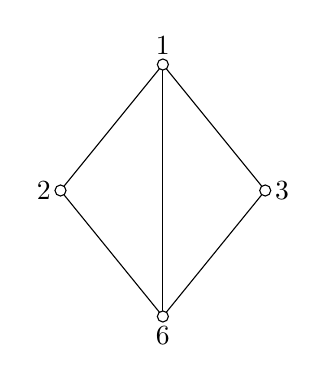
\begin{tikzpicture}
    \coordinate (top) at (0,1.6); \coordinate (left) at (-1.3,0);
    \coordinate (right) at (1.3,0); \coordinate (bot) at (0,-1.6);
    \draw (top) -- (bot); \draw (top) -- (left) -- (bot); \draw (top)
    -- (right) -- (bot); \foreach \p in {top,left,right,bot} {
      \fill[white] (\p) circle (2pt); \draw (\p) circle (2pt); }
    \node[above] at (top) {$1$}; \node[left] at (left) {$2$};
    \node[right] at (right) {$3$}; \node[below] at (bot) {$6$};
  \end{tikzpicture}
  \qquad\qquad
  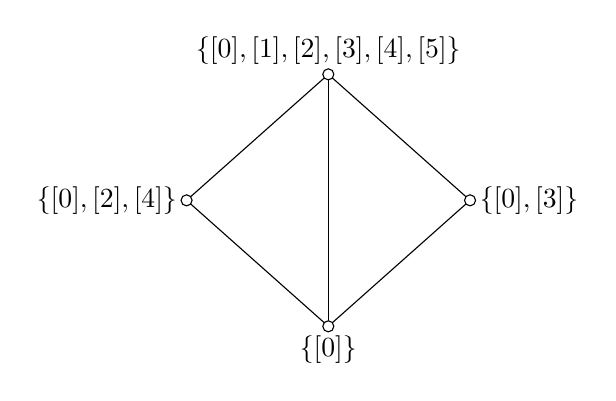
\begin{tikzpicture}
    \coordinate (top) at (0,1.6); \coordinate (left) at (-1.8,0);
    \coordinate (right) at (1.8,0); \coordinate (bot) at (0,-1.6);
    \draw (top) -- (bot); \draw (top) -- (left) -- (bot); \draw (top)
    -- (right) -- (bot); \foreach \p in {top,left,right,bot} {
      \fill[white] (\p) circle (2pt); \draw (\p) circle (2pt); }
    \node[above] at (top) {$\{[0],[1],[2],[3],[4],[5]\}$}; \node[left]
    at (left) {$\{[0],[2],[4]\}$}; \node[right] at (right)
    {$\{[0],[3]\}$}; \node[below] at (bot) {$\{[0]\}$};
  \end{tikzpicture}
\end{center}
where lines connect multiples in one picture and subsets in the other.
The reader will draw the lattice of subgroups of $S_3$, noting that it
looks completely different from the one for $\Z/6\Z$.

Contemplating subgroups of cyclic groups has pretty (and useful)
`number-theoretic' consequences; cf.\ \Cref{exer:groups:euler-totient-sum-formula}.

\subsection{Monomorphisms}
\label{subsec:groups:monomorphisms}
I end this section with some categorical considerations.

If $H$ is a subgroup of $G$, the inclusion $H \hookrightarrow G$ is an
example of a \emph{monomorphism} in $\categ{Grp}$ in the `categorical'
sense of \S{}\ref{subsec:prelims:morphisms:monomorphisms-and-epimorphisms}. In fact, it is easy to characterize all
monomorphisms $\varphi \in \Hom_{\categ{Grp}}(G,G')$ (where $G$, $G'$
are any groups):

\begin{prop}{The following are equivalent:
\begin{enumerate}[label=(\alph*)]
  \item $\varphi$ is a monomorphism;
  \item $\ker\varphi = \{e_G\}$;
  \item $\varphi : G \to G'$ is injective (as a set-function).
  \end{enumerate}}{prop:groups:monomorphism-characterization}
\end{prop}
\begin{proof}
  (a) $\implies$ (b): Assume (a) holds, and consider the two parallel
  compositions
  \[
    \begin{tikzcd}
      \ker\varphi \arrow[r, shift left, "i"] \arrow[r, shift right,
      "e"'] & G \arrow[r, "\varphi"] & G',
    \end{tikzcd}
  \]
  where $i$ is the inclusion and $e$ is the trivial map. Both
  $\varphi \circ i$ and $\varphi \circ e$ are the trivial map; since
  $\varphi$ is a monomorphism, this implies $i = e$. But $i = e$
  implies that $\ker\varphi$ is trivial, that is, (b) holds.

  (b) $\implies$ (c): Assume $\ker\varphi = \{e_G\}$. Then
  \[
    \varphi(g_1) = \varphi(g_2) \implies \varphi(g_1)\varphi(g_2)^{-1}
    = e_{G'} \implies \varphi(g_1 g_2^{-1}) = e_{G'} \implies g_1
    g_2^{-1} \in \ker\varphi \implies g_1 g_2^{-1} = e_G \implies g_1
    = g_2.
  \]
  This shows that $\varphi$ is injective, as needed.

  (c) $\implies$ (a): If $\varphi$ is injective, then it satisfies the
  defining property for monomorphisms in $\categ{Set}$: that is, for
  any set $Z$ and any two set-functions $\alpha', \alpha'' : Z \to G$,
  \[
    \varphi \circ \alpha' = \varphi \circ \alpha'' \iff \alpha' =
    \alpha''.
  \]
  This must hold in particular if $Z$ has a group structure and
  $\alpha'$, $\alpha''$ are group homomorphisms, so $\varphi$ is a
  monomorphism in $\categ{Grp}$.
\end{proof}

The equivalence (a) $\iff$ (c) may lead the reader to think that from
the point of view of monomorphisms, $\categ{Grp}$ and $\categ{Set}$
are pretty much alike. This is not quite so: while it is true that
homomorphisms with a left-inverse are necessarily monomorphisms, as in
$\categ{Set}$ (cf.\ \Cref{exer:groups:left-inverse-implies-monomorphism}), the converse is not true in
$\categ{Grp}$ (cf.\ \Cref{exer:groups:z3z-to-s3-no-left-inverse}).

\subsection*{Exercises}

\begin{exer}{$\lnot$}{exer:groups:matrix-subgroups-inclusions}
  (If you know about matrices.) The group of invertible $n \times n$
  matrices with entries in $\R$ is denoted $\mathrm{GL}_n(\R)$
  (\Cref{exam:groups:gln-matrices}). Similarly, $\mathrm{GL}_n(\C)$ denotes the
  group of $n \times n$ invertible matrices with complex
  entries. Consider the following sets of matrices:
  \begin{itemize}
  \item
    $\mathrm{SL}_n(\R) = \{M \in \mathrm{GL}_n(\R) \mid \det(M) =
    1\}$;
  \item
    $\mathrm{SL}_n(\C) = \{M \in \mathrm{GL}_n(\C)
    \mid \det(M) = 1\}$;
  \item
    $\mathrm{O}_n(\R) = \{M \in \mathrm{GL}_n(\R) \mid MM^t = M^tM =
    I_n\}$;
  \item
    $\mathrm{SO}_n(\R) = \{M \in \mathrm{O}_n(\R) \mid \det(M) = 1\}$;
  \item
    $\mathrm{U}(n) = \{M \in \mathrm{GL}_n(\C) \mid MM^\dagger
    = M^\dagger M = I_n\}$;
  \item $\mathrm{SU}(n) = \{M \in \mathrm{U}(n) \mid \det(M) = 1\}$.
  \end{itemize}
  Here $I_n$ stands for the $n \times n$ identity matrix, $M^t$ is the
  \emph{transpose} of $M$, $M^\dagger$ is the \emph{conjugate
    transpose} of $M$, and $\det(M)$ denotes the
  \emph{determinant}\footnote{If you are not familiar with some of
    these notions, that's ok: leave this exercise and similar ones
    alone if that is the case. We will come back to linear algebra and
    matrices in \Cref{chap:linalg} and following.} of $M$. Find all possible
  inclusions among these sets, and prove that in every case the
  smaller set is a subgroup of the larger one.

  These sets of matrices have compelling geometric interpretations:
  for example, $\mathrm{SO}_3(\R)$ is the group of `rotations' in
  $\R^3$. [\ref{exer:groups:sln-normal-in-gln}, \ref{exer:groups:on-preserves-lengths-angles}, \ref{exer:rings:matrix-ring}, \ref{exer:linalg:6.16}]
\end{exer}
\begin{exer}{$\lnot$}{exer:groups:upper-triangular-subgroup}
  Prove that the set of $2 \times 2$ matrices
  \[
    \begin{pmatrix} a & b \\ 0 & d \end{pmatrix}
  \]
  with $a, b, d$ in $\C$ and $ad \neq 0$ is a subgroup of
  $\mathrm{GL}_2(\C)$. More generally, prove that the set of
  $n \times n$ complex matrices $(a_{ij})_{1 \leq i,j \leq n}$ with
  $a_{ij} = 0$ for $i > j$ and $a_{11} \cdots a_{nn} \neq 0$ is a
  subgroup of $\mathrm{GL}_n(\C)$. (These matrices are called
  `upper triangular', for evident reasons.) [\ref{exer:groups2:gl2c-union-of-conjugates-of-borel}]
\end{exer}
\begin{exer}{$\lnot$}{exer:groups:su2-sphere}
  Prove that every matrix in $\mathrm{SU}(2)$ may be written in the
  form
  \[
    \begin{pmatrix} a+bi & c+di \\ -c+di & a-bi \end{pmatrix}
  \]
  where $a,b,c,d \in \R$ and $a^2+b^2+c^2+d^2=1$. (Thus,
  $\mathrm{SU}(2)$ may be realized as a three-dimensional sphere
  embedded in $\R^4$; in particular, it is simply connected.) [\ref{exer:groups:so3-su2-mod-plusminus-i},
  \ref{exer:rings:quaternion-norm}]
\end{exer}
\begin{exer}{\exerused}{exer:groups:exponential-image-cyclic}
  Let $G$ be a group, and let $g \in G$. Verify that the image of the
  exponential map $\epsilon_g : \Z \to G$ is a cyclic group (in the
  sense of \Cref{defn:groups:cyclic}). [\S{}\ref{subsec:groups:example-subgroup-generated-by-a-subset}, \S{}\ref{subsec:groups:example}]
\end{exer}
\begin{exer}{}{exer:groups:nth-powers-subgroup-commutative}
  Let $G$ be a commutative group, and let $n > 0$ be an integer. Prove
  that $\{g^n \mid g \in G\}$ is a subgroup of $G$. Prove that this is
  not necessarily the case if $G$ is not commutative.
\end{exer}
\begin{exer}{}{exer:groups:union-of-subgroups}
  Prove that the union of a family of subgroups of a group $G$ is not
  necessarily a subgroup of $G$. In fact:
  \begin{itemize}
  \item Let $H$, $H'$ be subgroups of a group $G$. Prove that
    $H \cup H'$ is a subgroup of $G$ only if $H \subseteq H'$ or
    $H' \subseteq H$.
  \item On the other hand, let
    $H_0 \subseteq H_1 \subseteq H_2 \subseteq \dots$ be subgroups of
    a group $G$. Prove that $\bigcup_{i \geq 0} H_i$ is a subgroup of
    $G$.
  \end{itemize}
\end{exer}
\begin{exer}{$\lnot$}{exer:groups:inn-cyclic-iff-abelian}
  Show that \emph{inner automorphisms} (cf.\ \Cref{exer:groups:inner-automorphisms}) form a
  subgroup of $\Aut(G)$; this subgroup is denoted
  $\operatorname{Inn}(G)$. Prove that $\operatorname{Inn}(G)$ is
  cyclic if and only if $\operatorname{Inn}(G)$ is trivial if and only
  if $G$ is abelian. (Hint: Assume that $\operatorname{Inn}(G)$ is
  cyclic; with notation as in \Cref{exer:groups:inner-automorphisms}, this means that there
  exists an element $a \in G$ such that
  $\forall g \in G\ \exists n \in \Z\ \gamma_g = \gamma_a^n$. In
  particular, $gag^{-1} = a^naa^{-n} = a$. Thus $a$ commutes with
  every $g$ in $G$. Therefore\dots.) Deduce that if
  $\Aut(G)$ is cyclic, then $G$ is abelian. [\ref{exer:groups:normal-iff-inn-stabilizes},
  \ref{exer:groups2:quot-ctr-iso-inn}]
\end{exer}
\begin{exer}{}{exer:groups:finitely-generated-abelian-surjection}
  Prove that an \emph{abelian} group $G$ is finitely generated if and
  only if there is a surjective homomorphism
  \[
    \underbrace{\Z \oplus \cdots \oplus \Z}_{n\text{ times}}
    \twoheadrightarrow G
  \]
  for some $n$.
\end{exer}
\begin{exer}{}{exer:groups:q-finitely-generated-subgroups-cyclic}
  Prove that every finitely generated subgroup of $\Q$ is cyclic.
  Prove that $\Q$ is not finitely generated.
\end{exer}
\begin{exer}{$\lnot$}{exer:groups:sl2z-generated-by-s-t}
  The set of $2 \times 2$ matrices with integer entries and
  determinant $1$ is denoted $\mathrm{SL}_2(\Z)$:
  \[
    \mathrm{SL}_2(\Z) = \left\{ \begin{pmatrix} a & b \\ c &
        d \end{pmatrix} \text{ such that } a,b,c,d \in \Z,\ ad-bc=1
    \right\}.
  \]
  Prove that $\mathrm{SL}_2(\Z)$ is generated by the matrices
  \[
    s = \begin{pmatrix} 0 & -1 \\ 1 & 0 \end{pmatrix} \quad \text{and}
    \quad t = \begin{pmatrix} 1 & 1 \\ 0 & 1 \end{pmatrix}.
  \]
  (Hint: This is a little tricky. Let $H$ be the subgroup generated by
  $s$ and $t$. Given a matrix
  $m = \begin{pmatrix} a & b \\ c & d \end{pmatrix}$ in
  $\mathrm{SL}_2(\Z)$, it suffices to show that you can obtain the
  identity by multiplying $m$ by suitably chosen elements of $H$.
  Prove that $\begin{pmatrix} 1 & -q \\ 0 & 1 \end{pmatrix}$ and
  $\begin{pmatrix} 1 & 0 \\ -q & 1 \end{pmatrix}$ are in $H$, and note
  that
  \[
    \begin{pmatrix} a & b \\ c & d \end{pmatrix}
    \begin{pmatrix} 1 & -q \\ 0 & 1 \end{pmatrix} = \begin{pmatrix} a
      & b-qa \\ c & d-qc \end{pmatrix} \quad \text{and} \quad
    \begin{pmatrix} a & b \\ c & d \end{pmatrix}
    \begin{pmatrix} 1 & 0 \\ -q & 1 \end{pmatrix} = \begin{pmatrix}
      a-qb & b \\ c-qd & d \end{pmatrix}.
  \]
  Note that if $c$ and $d$ are both nonzero, one of these two
  operations may be used to decrease the absolute value of one of
  them. Argue that suitable applications of these operations reduce to
  the case in which $c=0$ or $d=0$. Prove directly that $m \in H$ in
  that case.) [\ref{exer:groups:psl2z-modular-group}]
\end{exer}
\begin{exer}{}{exer:groups:s3-not-coproduct-of-cyclic}
  Since direct sums are coproducts in $\categ{Ab}$, the classification
  theorem for abelian groups mentioned in the text says that every
  finitely generated abelian group is a coproduct of cyclic groups in
  $\categ{Ab}$. The reader may be tempted to conjecture that every
  finitely generated group is a coproduct in $\categ{Grp}$. Show that
  this is not the case, by proving that $S_3$ is not a coproduct of
  cyclic groups.
\end{exer}
\begin{exer}{}{exer:groups:mn-generated-subgroup-of-z}
  Let $m$, $n$ be positive integers, and consider the subgroup
  $\langle m,n \rangle$ of $\Z$ they generate. By \Cref{prop:groups:subgroups-of-z},
  \[
    \langle m,n \rangle = d\Z
  \]
  for some positive integer $d$. What is $d$, in relation to $m$, $n$?
\end{exer}
\begin{exer}{$\lnot$}{exer:groups:lattices-c2c2-c4-s3-c6}
  Draw and compare the lattices of subgroups of $C_2 \times C_2$ and
  $C_4$. Draw the lattice of subgroups of $S_3$, and compare it with
  the one for $C_6$. [\ref{exer:groups:s3-normal-subgroups}]
\end{exer}
\begin{exer}{\exerused}{exer:groups:euler-totient-sum-formula}
  If $m$ is a positive integer, denote by $\varphi(m)$ the number of
  positive integers $r \leq m$ that are relatively prime to $m$ (that
  is, for which the gcd of $r$ and $m$ is $1$); this is called Euler's
  $\varphi$- (or `totient') function. For example, $\varphi(12) =
  4$. In other words, $\varphi(m)$ is the order of the group
  $(\Z/m\Z)^*$; cf.\ \Cref{prop:groups:units-group}.

  Put together the following observations:
  \begin{itemize}
  \item $\varphi(m) = $ the number of generators of $C_m$,
  \item every element of $C_n$ generates a subgroup of $C_n$,
  \item the discussion following \Cref{prop:groups:subgroups-of-znz} (in particular,
    every subgroup of $C_n$ is isomorphic to $C_m$, for some
    $m \mid n$),
  \end{itemize}
  to obtain a proof of the formula
  \[
    \sum_{m>0,\, m\mid n} \varphi(m) = n.
  \]
  (For example,
  $\varphi(1)+\varphi(2)+\varphi(3)+\varphi(4)+\varphi(6)+\varphi(12)
  = 1+1+2+2+2+4 = 12$.) [\ref{exer:groups:aut-cn-euler-phi}, $\S$\ref{subsec:groups:example-subgroups-of-cyclic-groups}, \ref{exer:groups:n-divides-phi-an-minus-1}, \ref{exer:irred:crt-znz-decomp-and-totient-formula}, $\S$\ref{subsec:fields:cyclotomic-polynomials-and-fields}]
\end{exer}
\begin{exer}{\exerused}{exer:groups:left-inverse-implies-monomorphism}
  Prove that if a group homomorphism $\varphi : G \to G'$ has a
  left-inverse, that is, a group homomorphism $\psi : G' \to G$ such
  that $\psi \circ \varphi = \id_G$, then $\varphi$ is a
  monomorphism.  [\S{}\ref{subsec:groups:monomorphisms}, \ref{exer:groups:z3z-to-s3-no-left-inverse}]
\end{exer}
\begin{exer}{\exerused}{exer:groups:z3z-to-s3-no-left-inverse}
  Counterpoint to \Cref{exer:groups:left-inverse-implies-monomorphism}: the homomorphism
  $\varphi : \Z/3\Z \to S_3$ given by
  \[
    \varphi([0]) = \begin{pmatrix}1&2&3\\1&2&3\end{pmatrix}, \quad
    \varphi([1]) = \begin{pmatrix}1&2&3\\3&1&2\end{pmatrix}, \quad
    \varphi([2]) = \begin{pmatrix}1&2&3\\2&3&1\end{pmatrix}
  \]
  is a monomorphism; show that it has no left-inverse in
  $\categ{Grp}$.  (Knowing about normal subgroups will make this
  problem particularly easy.) [\S{}\ref{subsec:groups:monomorphisms}]
\end{exer}

\section{Quotient groups}
\label{sec:groups:quotient-groups}


\subsection{Normal subgroups}
\label{subsec:groups:normal-subgroups}
Before tackling `quotient groups', I should clarify in what sense
kernels are \emph{special} subgroups, as claimed in \S{}\ref{subsec:groups:examples-kernel-and-image}.

\begin{defn}{Normal subgroup}{defn:groups:normal-subgroup}
  A subgroup $N$ of a group $G$ is \emph{normal} if $\forall g \in G$,
  $\forall n \in N$,
  \[
    gng^{-1} \in N.
  \]
\end{defn}

Note that \emph{every} subgroup of a commutative group is normal
(because then $\forall g \in G$, $gng^{-1} = n \in N$). However, in
general \emph{not all} subgroups are normal: examples may be found
already in $S_3$ (cf.\ \Cref{exer:groups:s3-normal-subgroups}). There exist noncommutative
groups in which every subgroup is normal (one example is the
`quaternionic group' $Q_8$; cf.\ \Cref{exer:rings:quaternions} (iv)), but they are
very rare.

\begin{lem}{If $\varphi : G \to G'$ is any group homomorphism, then
    $\ker\varphi$ is a normal subgroup of
    $G$.}{lem:groups:kernel-is-normal}
\end{lem}
\begin{proof}
  We already know that $\ker\varphi$ is a subgroup of $G$; to verify
  it is normal note that $\forall g \in G$,
  $\forall n \in \ker\varphi$
  \[
    \varphi(gng^{-1}) = \varphi(g)\varphi(n)\varphi(g^{-1}) =
    \varphi(g)e_{G'}\varphi(g)^{-1} = e_{G'},
  \]
  proving that $gng^{-1} \in \ker\varphi$.
\end{proof}

Loosely speaking, therefore, \emph{kernel $\implies$ normal}. In fact
more is true, as we will see in a little while; for now I don't want
to spoil the surprise for the reader. (Can the reader guess?)

There is a convenient shorthand to express conditions such as
normality: if $g \in G$ and $A \subseteq G$ is any subset, we denote
by $gA$, $Ag$, respectively, the following subsets of $G$:
\[
  gA := \{h \in G \mid (\exists a \in A) : h = ga\}, \qquad Ag := \{h
  \in G \mid (\exists a \in A) : h = ag\}.
\]
Then the normality condition can be expressed by
\[
  (\forall g \in G) : \quad gNg^{-1} \subseteq N,
\]
or in a number of other ways:
\[
  gNg^{-1} = N \quad \text{or} \quad gN \subseteq Ng \quad \text{or}
  \quad gN = Ng
\]
for all $g \in G$. The reader should check that these are indeed
equivalent conditions (\Cref{exer:groups:normality-conditions-equivalent}) and keep in mind that `$gN = Ng$'
does \emph{not} mean that $g$ commutes with every element of $N$; it
means that if $n \in N$, then there are elements $n', n'' \in N$, in
general different from $n$, such that $gn = n'g$ (so that
$gN \subseteq Ng$) and $ng = gn''$ (so that $Ng \subseteq gN$).

\subsection{Quotient group}
\label{subsec:groups:quotient-group}
Recall that we have the notion of a quotient of a \emph{set} by an
equivalence relation (\S{}\ref{subsec:prelims:equiv-relations}) and that this notion satisfies a
universal property (clumsily stated in \S{}\ref{subsec:prelims:quotients}). It is natural to
investigate this notion in $\categ{Grp}$.

We consider then an equivalence relation $\sim$ on (the set
underlying) a group $G$; we seek a group $G/\!\sim$ and a group
homomorphism $\pi : G \to G/\!\sim$ satisfying the appropriate
universal property, that is, initial with respect to group
homomorphisms $\varphi : G \to G'$ such that
$a \sim b \implies \varphi(a) = \varphi(b)$.

It is natural to try to construct the group $G/\!\sim$ by defining an
operation $\bullet$ on the \emph{set} $G/\!\sim$. The situation is
tightly constrained by the requirement that the quotient map
$\pi : G \to G/\!\sim$ (as in \S{}\ref{subsec:prelims:functions:monomorphisms-and-epimorphisms}) be a group homomorphism: for
if $[a] = \pi(a)$, $[b] = \pi(b)$ are elements of $G/\!\sim$ (that is,
equivalence classes with respect to $\sim$), then the homomorphism
condition \emph{forces}
\[ [a] \bullet [b] = \pi(a) \bullet \pi(b) = \pi(ab) = [ab].
\]
But is this operation well-defined? This amounts to conditions on the
equivalence relation, which we proceed to unearth.

For the operation to be well-defined `in the first factor', it is
necessary that if $[a] = [a']$, then $[ab] = [a'b]$ regardless of what
$b$ is; that is,
\[
  (\forall g \in G) : \quad a \sim a' \implies ag \sim a'g.
\]
Similarly, for the operation to be well-defined in the second factor
we need
\[
  (\forall g \in G) : \quad a \sim a' \implies ga \sim ga'.
\]
Luckily, this is all that there is to it:

\begin{prop}{With notation as above, the operation
    \[ [a] \bullet [b] := [ab]
\]
defines a group structure on $G/\!\sim$ if and only if
$\forall a, a', g \in G$
\[
  a \sim a' \implies ga \sim ga' \text{ and } ag \sim a'g.
\]
In this case the quotient function $\pi : G \to G/\!\sim$ is a
homomorphism and is universal with respect to homomorphisms
$\varphi : G \to G'$ such that
$a \sim a' \implies \varphi(a) =
\varphi(a')$.}{prop:groups:quotient-group-universal-property}
\end{prop}
\begin{proof}
  We have already noted that the condition is necessary. To prove it
  is sufficient, with the stated consequences, assume
  $\forall a, a', g \in G$
  \[
    a \sim a' \implies ga \sim ga' \text{ and } ag \sim a'g.
  \]
  Then the operation
  \[ [a] \bullet [b] := [ab]
  \]
  is well-defined, and we have to verify that it defines a group
  structure on $G/\!\sim$. The associativity of $\bullet$ is inherited
  from the associativity of $G$: $\forall a,b,c \in G$
  \[
    ([a] \bullet [b]) \bullet [c] = [ab] \bullet [c] = [(ab)c] =
    [a(bc)] = [a] \bullet [bc] = [a] \bullet ([b] \bullet [c]).
  \]
  The class $[e_G]$ is an identity with respect to this operation:
  $\forall g \in G$
  \[ [g] \bullet [e_G] = [ge_G] = [g], \qquad [e_G] \bullet [g] =
    [e_Gg] = [g].
  \]
  The class $[g^{-1}]$ is the inverse of $[g]$:
  \[ [g^{-1}] \bullet [g] = [g^{-1}g] = [e_G], \qquad [g] \bullet
    [g^{-1}] = [gg^{-1}] = [e_G].
  \]
  This shows $G/\!\sim$ is indeed a group, and we have already
  observed that $\pi : G \to G/\!\sim$ is a homomorphism: this is what
  led us to the definition of $\bullet$.

  To prove that $G/\!\sim$ satisfies the universal property, assume
  \[
    \varphi : G \to G'
  \]
  is a group homomorphism such that
  $a \sim a' \implies \varphi(a) = \varphi(a')$. Since (cf.\
  \S{}\ref{subsec:prelims:quotients}) the \emph{set} $G/\!\sim$ satisfies the corresponding
  universal property in $\categ{Set}$, we know that there exists a
  unique set-function
  \[
    \bar\varphi : G/\!\sim \to G',
  \]
  defined\footnote{The point of \S{}\ref{subsec:prelims:quotients} is precisely that this
    function is well-defined.} by $\bar\varphi([a]) := \varphi(a)$. So
  we only need to check that this function $\bar\varphi$ is in fact a
  group homomorphism, and this is immediate:
  \[
    \bar\varphi([a] \bullet [b]) = \bar\varphi([ab]) = \varphi(ab) =
    \varphi(a)\varphi(b) = \bar\varphi([a])\bar\varphi([b])
  \]
  for all $[a], [b] \in G/\!\sim$, as needed.
\end{proof}

I will say that $\sim$ is \emph{compatible} with the group structure
of $G$ if the condition given in
Proposition~\ref{prop:groups:quotient-group-universal-property} holds.
Since the operation $\bullet$ on the quotient $G/\!\sim$ is uniquely
determined by the operation on $G$, I yield to the usual abuse of
language and omit it. If $\sim$ is compatible, I will call $G/\!\sim$
the \emph{quotient group} of $G$ by $\sim$.

\subsection{Cosets}
\label{subsec:groups:cosets}
The conditions obtained in
Proposition~\ref{prop:groups:quotient-group-universal-property},
\begin{align}
  \tag{$\dagger$} (\forall g \in G) &: \quad a \sim b \implies ga \sim gb, \\
  \tag{$\dagger\dagger$} (\forall g \in G) &: \quad a \sim b \implies ag \sim bg,
\end{align}
lead to a complete description of \emph{all} compatible relations on a
group $G$. In fact, each of these two conditions leads to a
description of the relations satisfying it, and we will analyze them
separately; the reader should keep in mind that we have a group
structure on $G/\!\sim$ only if \emph{both} are satisfied.

Let's begin with $(\dagger)$. Here is the description:

\begin{prop}{Let $\sim$ be an equivalence relation on a group $G$,
satisfying $(\dagger)$. Then
\begin{itemize}
\item the equivalence class of $e_G$ is a subgroup $H$ of $G$; and
\item $a \sim b \iff a^{-1}b \in H \iff aH = bH$.
\end{itemize}}{prop:groups:coset-description-dagger}
\end{prop}
\begin{proof}
  Let $H \subseteq G$ be the equivalence class of the identity;
  $H \neq \emptyset$ as $e_G \in H$. For $a, b \in H$, we have
  $e_G \sim b$ and hence $b^{-1} \sim e_G$ (applying $(\dagger)$,
  multiplying on the left by $b^{-1}$); hence $ab^{-1} \sim a$ (by
  $(\dagger)$ again, multiplying on the left by $a$); and hence
  \[
    ab^{-1} \sim a \sim e_G
  \]
  by the transitivity of $\sim$ and since $a \in H$. This shows that
  $ab^{-1} \in H$ for all $a, b \in H$, proving that $H$ is a subgroup
  (by Proposition~\ref{prop:groups:subgroup-criterion}).

  Next, assume $a, b \in G$ and $a \sim b$. Multiplying on the left by
  $a^{-1}$, $(\dagger)$ implies $e_G \sim a^{-1}b$, that is,
  $a^{-1}b \in H$. Since $H$ is closed under the operation, this
  implies $a^{-1}bH \subseteq H$, hence $bH \subseteq aH$; as $\sim$
  is symmetric, the same reasoning gives $aH \subseteq bH$; and hence
  $aH = bH$. Thus, we have proved
  \[
    a \sim b \implies a^{-1}b \in H \implies aH = bH.
  \]
  Finally, assume $aH = bH$. Then $a = ae_G \in bH$, and hence
  $a^{-1}b \in H$. By definition of $H$, this means
  $e_G \sim a^{-1}b$.  Multiplying on the left by $a$ shows (by
  $(\dagger)$ again) that $a \sim b$, completing the proof.
\end{proof}

Proposition~\ref{prop:groups:coset-description-dagger} shows that the
equivalence classes of an equivalence relation satisfying $(\dagger)$
are in fact all of the form
\[
  aH
\]
for a fixed subgroup $H$, as $a$ ranges in $G$. These important
subsets determined by a subgroup $H$ deserve a name.

\begin{defn}{Left-/right-cosets}{defn:groups:cosets}
  The \emph{left-cosets} of a subgroup $H$ in a group $G$ are the sets
  $aH$, for $a \in G$. The \emph{right-cosets} of $H$ are the sets
  $Ha$, $a \in G$.
\end{defn}

Now, a `converse' to
Proposition~\ref{prop:groups:coset-description-dagger} holds:

\begin{prop}{If $H$ is any subgroup of a group $G$, the relation
$\sim_L$ defined by
\[
  (\forall a, b \in G) : \quad a \sim_L b \iff a^{-1}b \in H
\]
is an equivalence relation satisfying
$(\dagger)$.}{prop:groups:sim-l-satisfies-dagger}
\end{prop}
\begin{proof}
  This is straightforward and is mostly left to the reader
  (\Cref{exer:groups:prove-prop-7-6}). To see that the relation satisfies $(\dagger)$, note
  that
  \[
    a \sim_L b \implies a^{-1}b \in H \implies a^{-1}(g^{-1}g)b \in H
    \implies (ga)^{-1}(gb) \in H \implies ga \sim_L gb
  \]
  for all $g \in G$.
\end{proof}

Taken together,
Propositions~\ref{prop:groups:coset-description-dagger}
and~\ref{prop:groups:sim-l-satisfies-dagger} show

\begin{prop}{There is a one-to-one correspondence between subgroups of
    $G$ and equivalence relations on $G$ satisfying $(\dagger)$; for
    the relation $\sim_L$ corresponding to a subgroup $H$,
    $G/\!\sim_L$ may be described as the set of left-cosets $aH$ of
    $H$.}{prop:groups:subgroups-correspond-to-dagger-relations}
\end{prop}

The reader should have no difficulty producing the mirror statements
(and proofs) giving a similarly exhaustive description of all
equivalence relations satisfying $(\dagger\dagger)$. The end result
will be

\begin{prop}{There is a one-to-one correspondence between subgroups of
    $G$ and equivalence relations on $G$ satisfying
    $(\dagger\dagger)$; for the relation $\sim_R$ corresponding to a
    subgroup $H$, $G/\!\sim_R$ may be described as the set of
    right-cosets $Ha$ of
    $H$.}{prop:groups:subgroups-correspond-to-daggerdagger-relations}
\end{prop}
The relation corresponding to $H$ in this second way is defined by
\[
  a \sim_R b \iff ab^{-1} \in H \iff Ha = Hb.
\]

What may be surprising at first is that the relations $\sim_L$ and
$\sim_R$ corresponding to the \emph{same} subgroup $H$ may very well
not be the same relation. That is, left-cosets and right-cosets of a
subgroup need not coincide. Of course $eH = He = H$, and more
generally
\[
  (\forall h \in H) : \quad hH = Hh = H.
\]
Further
\[
  (\forall a \in G) : \quad a \in aH \cap Ha;
\]
hence, if $aH = Hb$ for any $b$, then in fact necessarily $aH = Ha$.
This is of course automatically true if $G$ is commutative, but it is
simply not the case in general.

\begin{exam}{}{exam:groups:s3-left-right-cosets}
  Let $G = S_3$, and let $H$ be the subgroup consisting of the
  identity and the $1 \leftrightarrow 2$ switch:
  \[
    H = \left\{ \begin{pmatrix}1&2&3\\1&2&3\end{pmatrix},
      \begin{pmatrix}1&2&3\\2&1&3\end{pmatrix} \right\}.
  \]
  Then
  \[
    \begin{pmatrix}1&2&3\\3&1&2\end{pmatrix} H =
    \left\{ \begin{pmatrix}1&2&3\\3&1&2\end{pmatrix},
      \begin{pmatrix}1&2&3\\3&2&1\end{pmatrix} \right\},
  \]
  while
  \[
    H \begin{pmatrix}1&2&3\\3&1&2\end{pmatrix} =
    \left\{ \begin{pmatrix}1&2&3\\3&1&2\end{pmatrix},
      \begin{pmatrix}1&2&3\\1&3&2\end{pmatrix} \right\}.
  \]
  This state of affairs simply reflects the fact that the two
  conditions $(\dagger)$ and $(\dagger\dagger)$ are different: there
  is no reason to expect that if one holds, the other one should also
  hold (unless $G$ is commutative, of course). Once more, keep in mind
  that \emph{both} have to hold for the quotient $G/\!\sim$ to be a
  group, compatibly with the operation in $G$; cf.\
  Proposition~\ref{prop:groups:quotient-group-universal-property}.
\end{exam}

\subsection{Quotient by normal subgroups}
\label{subsec:groups:quotient-by-normal-subgroups}
To stress the main point again, an arbitrary subgroup $H$ of $G$ leads
to two partitions of $G$, which we have denoted
\[
  G/\!\sim_L\, = \{aH \mid a \in G\}, \qquad G/\!\sim_R\, = \{Ha \mid
  a \in G\}.
\]
The relation $\sim_L$ satisfies property $(\dagger)$ listed at the
beginning of \S{}\ref{subsec:groups:cosets}; $\sim_R$ satisfies $(\dagger\dagger)$. A priori,
these relations, and hence the corresponding partitions, are
different.

The condition that $\sim_L$ and $\sim_R$ coincide (as is necessarily
the case, for example, if $G$ is commutative) translates into a
condition on $H$: for such `special' subgroups, $(\dagger)$ and
$(\dagger\dagger)$ get back together. The good news is that this
condition is easy to identify and is not new to the reader.

\begin{prop}{The relations $\sim_L$, $\sim_R$ corresponding to a
    subgroup $H$ coincide if and only if $H$ is
    normal.}{prop:groups:sim-l-sim-r-coincide-iff-normal}
\end{prop}
\begin{proof}
  Two relations coincide if the corresponding partitions agree.
  Therefore
  \[
    \sim_L\, = \sim_R \iff \text{left- and right-cosets of } H \text{
      coincide} \iff (\forall g \in G) : gH = Hg.
  \]
  But this is one of the equivalent conditions defining the notion of
  normal subgroup (cf.\ \S{}\ref{subsec:groups:normal-subgroups}), proving the statement.
\end{proof}

The innocent-looking
Proposition~\ref{prop:groups:sim-l-sim-r-coincide-iff-normal} is of
fundamental importance. If $H$ is normal, then the one equivalence
relation $\sim\, = \sim_L\, = \sim_R$ corresponding to $H$ satisfies
both $(\dagger)$ and $(\dagger\dagger)$ (by
Proposition~\ref{prop:groups:coset-description-dagger} and its mirror
statement), and hence (by
Proposition~\ref{prop:groups:quotient-group-universal-property}) the
quotient
\[
  G/\!\sim\, = \{aH \mid a \in G\} = \{Ha \mid a \in G\}
\]
has a natural group structure.

\begin{defn}{Quotient group of $G$ modulo $H$}{defn:groups:quotient-group-modulo-h}
  Let $H$ be a normal subgroup of a group $G$. The \emph{quotient
    group of $G$ modulo $H$}, denoted\footnote{In a large display I
    sometime use the full `fraction' notation $\frac{G}{H}$.} $G/H$,
  is the group $G/\!\sim$ obtained from the relation $\sim$ defined
  above. In terms of (left-)cosets, the product in $G/H$ is defined by
  \[
    (aH)(bH) := (ab)H.
  \]
  The identity element $e_{G/H}$ of the quotient group $G/H$ is the
  coset of the identity, $e_GH = H$.
\end{defn}

By Proposition~\ref{prop:groups:quotient-group-universal-property},
the quotient function
\[
  \pi : G \to G/H
\]
sending $g \in G$ to $gH = Hg$ is a group homomorphism and is
universal with respect to group homomorphisms $\varphi : G \to G'$
such that $aH = bH \implies \varphi(a) = \varphi(b)$. This universal
property is extremely useful, so I will grace it with theorem status:

\begin{thm}{Let $H$ be a normal subgroup of a group $G$. Then for
    every group homomorphism $\varphi : G \to G'$ such that
    $H \subseteq \ker\varphi$ there exists a unique group homomorphism
    $\bar\varphi : G/H \to G'$ so that the diagram
    commutes.}{thm:groups:quotient-universal-property}
  \[
    \begin{tikzcd}
      G \arrow[r, "\varphi"] \arrow[d, "\pi"'] & G' \\
      G/H \arrow[ur, dashed, "\exists ! \bar\varphi"'] &
    \end{tikzcd}
  \]
\end{thm}
\begin{proof}
  We only need to match the stated universal property with the one we
  proved in
  Proposition~\ref{prop:groups:quotient-group-universal-property}, and
  indeed,
  \[
    H \subseteq \ker\varphi \iff (\forall h \in H) : \varphi(h) =
    e_{G'}
  \]
  is equivalent to
  \[
    (\forall a, b \in G) : ab^{-1} \in H \implies \varphi(ab^{-1}) =
    e_{G'}
  \]
  that is, to
  \[
    (\forall a, b \in G) : ab^{-1} \in H \implies \varphi(a) =
    \varphi(b)
  \]
  and finally, keeping in mind how the relation $\sim$ corresponding
  to $H$ is defined,
  \[
    (\forall a, b \in G) : a \sim b \implies \varphi(a) = \varphi(b),
  \]
  the condition giving the universal property in
  Proposition~\ref{prop:groups:quotient-group-universal-property}.
\end{proof}

\subsection{Example}
\label{subsec:groups:example}
The reader is already very familiar with an important class of
examples: the cyclic groups $\Z/n\Z$. Indeed, in \S{}\ref{subsec:groups:cyclic-groups-and-modular-arithmetic} we defined
$\Z/n\Z$ as the set of equivalence classes in $\Z$ with respect to the
congruence equivalence relation
\[
  (\forall a, b \in \Z) : \quad a \equiv b \mod n \iff n \mid (b-a).
\]
Now we recognize that $n \mid (b-a)$ is equivalent to
\[
  b - a \in n\Z,
\]
which is the relation $\sim_L$ corresponding (in `abelian' notation)
to the subgroup $n\Z$ of $\Z$. This subgroup is of course normal,
since $\Z$ is abelian. The `congruence classes mod $n$' are nothing
but the cosets of the subgroup $n\Z$ in $\Z$; using abelian notation
for cosets, we could write
\[ [a]_n = a + (n\Z).
\]
Of course the operation defined on $\Z/n\Z$ in \S{}\ref{subsec:groups:cyclic-groups-and-modular-arithmetic} matches
precisely the one defined above for quotient groups. This justifies
the notation $\Z/n\Z$ introduced in \S{}\ref{subsec:groups:cyclic-groups-and-modular-arithmetic}.

The reader can already appreciate in this simple context the
usefulness of
Theorem~\ref{thm:groups:quotient-universal-property}. Let $g \in G$ be
an element of order $n$ and consider the exponential map
\[
  \epsilon_g : \Z \to G, \quad N \mapsto g^N.
\]
By Corollary~\ref{coro:groups:order-multiple},
\[
  \ker\epsilon_g = \{N \in \Z \mid N \text{ is a multiple of } |g|\} =
  n\Z.
\]
Theorem~\ref{thm:groups:quotient-universal-property} then implies
right away that $\epsilon_g$ factors through the quotient:
\[
  \begin{tikzcd}
    \Z \arrow[r, "\epsilon_g"] \arrow[d, "\pi_n"'] & G \\
    \Z/n\Z \arrow[ur, dashed, "\exists ! \bar\epsilon_g"'] &
  \end{tikzcd}
\]
That is, there is an induced map
\[
  \Z/n\Z \to \langle g \rangle.
\]
In fact, the `canonical decomposition' of \S{}\ref{subsec:prelims:canonical-decomposition} implies that this
is an isomorphism (verifying that $\langle g \rangle$ is cyclic in the
sense of \Cref{defn:groups:cyclic}, as the reader should have checked `by hand'
already in \Cref{exer:groups:exponential-image-cyclic}). We will formalize this observation in
general in the next section.

Also note that $|g| = n = |\langle g \rangle|$ in this case.

\subsection{\texorpdfstring{kernel $\Leftrightarrow$ normal}{kernel
    iff normal}}
\label{subsec:groups:kernel-iff-normal}
If $H$ is a normal subgroup, we have now constructed in gory detail a
group $G/H$ and a surjective homomorphism
\[
  \pi : G \to G/H.
\]
What is the kernel of $\pi$? The identity of $G/H$ is the coset
$e_GH$, that is, $H$ itself. Therefore
\[
  \ker\pi = \{g \in G \mid gH = H\} = H.
\]
This observation completes the circle of ideas begun in \S{}\ref{subsec:groups:normal-subgroups}: there
we had noticed that every kernel (of a group homomorphism) is a normal
subgroup; and now we have verified that every normal subgroup is in
fact a \emph{kernel} (of some group homomorphism). I encapsulate this
in the slogan
\[
  \text{kernel} \iff \text{normal}:
\]
in group theory\footnote{We will run into analogous observations in
  ring theory, where we will verify that kernels and \emph{ideals}
  coincide, and for modules, as kernels and \emph{submodules} again
  coincide.}, `kernel' and `normal subgroup' are equivalent concepts.

For example, every subgroup in an abelian group is the kernel of some
homomorphism: yet another indication that life is simpler in
$\categ{Ab}$ than in $\categ{Grp}$.

\subsection*{Exercises}

\begin{exer}{\exerused}{exer:groups:s3-normal-subgroups}
  List all subgroups of $S_3$ (cf.\ \Cref{exer:groups:lattices-c2c2-c4-s3-c6}) and determine which
  subgroups are normal and which are not normal. [\S{}\ref{subsec:groups:normal-subgroups}]
\end{exer}
\begin{exer}{}{exer:groups:image-not-necessarily-normal}
  Is the \emph{image} of a group homomorphism necessarily a normal
  subgroup of the target?
\end{exer}
\begin{exer}{\exerused}{exer:groups:normality-conditions-equivalent}
  Verify that the equivalent conditions for normality given in \S{}\ref{subsec:groups:normal-subgroups}
  are indeed equivalent. [\S{}\ref{subsec:groups:normal-subgroups}]
\end{exer}
\begin{exer}{}{exer:groups:exercise-5-10-relation-compatible}
  Prove that the relation defined in \Cref{exer:groups:fab-quotient-by-2g} on a free abelian
  group $F = F^{ab}(A)$ is compatible with the group
  structure. Determine the quotient $F/\!\sim$ as a better known
  group.
\end{exer}
\begin{exer}{$\lnot$}{exer:groups:psl2z-modular-group}
  Define an equivalence relation $\sim$ on $\mathrm{SL}_2(\Z)$ by
  letting $A \sim A' \iff A' = \pm A$. Prove that $\sim$ is compatible
  with the group structure. The quotient $\mathrm{SL}_2(\Z)/\!\sim$ is
  denoted $\mathrm{PSL}_2(\Z)$ and is called the \emph{modular group};
  it would be a serious contender in a contest for `the most important
  group in mathematics', due to its role in algebraic geometry and
  number theory. Prove that $\mathrm{PSL}_2(\Z)$ is generated by the
  (cosets of the) matrices
  \[
    \begin{pmatrix} 0 & -1 \\ 1 & 0 \end{pmatrix} \quad \text{and}
    \quad
    \begin{pmatrix} 1 & -1 \\ 1 & 0 \end{pmatrix}.
  \]
  (You will not need to work very hard, if you use the result of
  \Cref{exer:groups:sl2z-generated-by-s-t}.) Note that the first has order $2$ in
  $\mathrm{PSL}_2(\Z)$, the second has order $3$, and their product
  has infinite order. [\ref{exer:groups:psl2z-coproduct-c2-c3}]
\end{exer}
\begin{exer}{}{exer:groups:gn-relation-equivalence-commutative}
  Let $G$ be a group, and let $n$ be a positive integer. Consider the
  relation
  \[
    a \sim b \iff (\exists g \in G)\ ab^{-1} = g^n.
  \]
  \begin{itemize}
  \item Show that in general $\sim$ is \emph{not} an equivalence
    relation.
  \item Prove that $\sim$ is an equivalence relation if $G$ is
    commutative, and determine the corresponding subgroup of $G$.
  \end{itemize}
\end{exer}
\begin{exer}{}{exer:groups:order-n-elements-generate-normal}
  Let $G$ be a group, $n$ a positive integer, and let $H \subseteq G$
  be the subgroup generated by all elements of order $n$ in $G$. Prove
  that $H$ is normal.
\end{exer}
\begin{exer}{\exerused}{exer:groups:prove-prop-7-6}
  Prove
  Proposition~\ref{prop:groups:sim-l-satisfies-dagger}. [\S{}\ref{subsec:groups:cosets}]
\end{exer}
\begin{exer}{}{exer:groups:mirror-statements-daggerdagger}
  State and prove the `mirror' statements of
  Propositions~\ref{prop:groups:coset-description-dagger}
  and~\ref{prop:groups:sim-l-satisfies-dagger}, leading to the
  description of relations satisfying $(\dagger\dagger)$.
\end{exer}
\begin{exer}{$\lnot$}{exer:groups:normal-iff-inn-stabilizes}
  Let $G$ be a group, and $H \subseteq G$ a subgroup. With notation as
  in \Cref{exer:groups:inn-cyclic-iff-abelian}, show that $H$ is normal in $G$ if and only if
  $\forall \gamma \in \operatorname{Inn}(G), \gamma(H) \subseteq H$.

  Conclude that if $H$ is normal in $G$, then there is an interesting
  homomorphism $\operatorname{Inn}(G) \to
  \Aut(H)$. [\ref{exer:groups:g-mod-h-to-aut-h}]
\end{exer}
\begin{exer}{\exerused}{exer:groups:commutator-subgroup-normal}
  Let $G$ be a group, and let $[G,G]$ be the subgroup of $G$ generated
  by all elements of the form $aba^{-1}b^{-1}$. (This is the
  \emph{commutator subgroup} of $G$; we will return to it in
  \S{}\ref{subsec:groups2:the-commutator-subgroup-derived-series-and-solvability}.) Prove that $[G,G]$ is normal in $G$. (Hint: With
  notation as in \Cref{exer:groups:inner-automorphisms},
  $g \cdot aba^{-1}b^{-1} \cdot g^{-1} = \gamma_g(aba^{-1}b^{-1})$.)
  Prove that $G/[G,G]$ is commutative. [\ref{exer:groups:free-mod-commutator-is-fab}, $\S$\ref{subsec:groups2:the-commutator-subgroup-derived-series-and-solvability}]
\end{exer}
\begin{exer}{\exerused}{exer:groups:free-mod-commutator-is-fab}
  Let $F = F(A)$ be a free group, and let $f : A \to G$ be a
  set-function from the set $A$ to a commutative group $G$. Prove that
  $f$ induces a unique homomorphism $F/[F,F] \to G$, where $[F,F]$ is
  the commutator subgroup of $F$ defined in \Cref{exer:groups:commutator-subgroup-normal}. (Use
  Theorem~\ref{thm:groups:quotient-universal-property}.) Conclude that
  $F/[F,F] \cong F^{ab}(A)$. (Use \Cref{prop:prelims:initial-final-unique}.) [\S{}\ref{subsec:groups:example-subgroups-of-cyclic-groups}, \ref{exer:groups:free-groups-isomorphic-implies-sets-isomorphic},
  \ref{exer:linalg:1.20}]
\end{exer}
\begin{exer}{$\lnot$}{exer:groups:free-groups-isomorphic-implies-sets-isomorphic}
  Let $A$, $B$ be sets and $F(A)$, $F(B)$ the corresponding free
  groups.  Assume $F(A) \cong F(B)$. If $A$ is finite, prove that $B$
  is also and $A \cong B$. (Use \Cref{exer:groups:free-mod-commutator-is-fab} to upgrade
  \Cref{exer:groups:fab-quotient-by-2g}.) [\ref{exer:groups:fab-quotient-by-2g}, \ref{exer:linalg:1.20}]
\end{exer}
\begin{exer}{}{exer:groups:inn-normal-in-aut}
  Let $G$ be a group. Prove that $\operatorname{Inn}(G)$ is a normal
  subgroup of $\Aut(G)$.
\end{exer}

\section{Canonical decomposition and Lagrange's theorem}
\label{sec:groups:canonical-decomposition-and-lagrange-s-theorem}

I will collect in this section a number of observations on the
structure of quotient groups. All these results are straightforward,
given the background work done so far. Some of them are often given
fancy names such as \emph{first isomorphism theorem} in the
literature; I am not too fond of such terminology: the universal
property proven in
Theorem~\ref{thm:groups:quotient-universal-property} is really the
only thing I need to take along, and it serves me wonderfully
well. The `isomorphism theorems' are all immediate applications of
this universal property.

\subsection{Canonical decomposition}
\label{subsec:groups:canonical-decomposition}
The first observation comes from the canonical decomposition for
set-functions, obtained in \S{}\ref{subsec:prelims:canonical-decomposition}: every set-function may be viewed
as the composition of a surjective map, followed by a bijective map,
followed by an injective map. We now know enough to state the
corresponding (very useful) result in $\categ{Grp}$:

\begin{thm}{Every group homomorphism $\varphi : G \to G'$ may be
    decomposed as follows, where the isomorphism $\bar\varphi$ in the
    middle is the homomorphism induced by $\varphi$ (as in
    Theorem~\ref{thm:groups:quotient-universal-property}):}{thm:groups:canonical-decomposition}
  \[
    \begin{tikzcd}
      G \arrow[rr, "\varphi", bend left=15] \arrow[r, two heads] &
      G/\ker\varphi \arrow[r, "\bar\varphi"', "\sim"] &
      \image\varphi \arrow[r, hook] & G'
    \end{tikzcd}
  \]
\end{thm}
\begin{proof}
  It is important that the reader agree that we have already proved
  anything that deserves to be proven here. We know that the
  projection on the left and the inclusion on the right are
  homomorphisms and $\bar\varphi$ comes from
  Theorem~\ref{thm:groups:quotient-universal-property}.  The
  decomposition is the same one obtained at the level of set-functions
  in \S{}\ref{subsec:prelims:canonical-decomposition}; in particular, the function in the middle is a
  bijection. Since bijective homomorphisms are isomorphisms
  (\Cref{prop:groups:iso-iff-bijection}), it is an isomorphism.
\end{proof}

Theorem~\ref{thm:groups:canonical-decomposition} should induce the
following Pavlovian reaction: exposed to any group homomorphism
$\varphi : G \to G'$, the reader should instantaneously view
$G/\ker\varphi$ as (canonically identified with) a subgroup of $G'$.
What is usually called the `first isomorphism theorem' is the
particular case corresponding to surjective homomorphisms:

\begin{coro}{Suppose $\varphi : G \to G'$ is a surjective group
homomorphism. Then
\[
  G' \cong \frac{G}{\ker\varphi}.
\]}{coro:groups:first-isomorphism-theorem}
\end{coro}
\begin{proof}
  $\image\varphi = G'$ in
  Theorem~\ref{thm:groups:canonical-decomposition}.
\end{proof}

This result is very useful---it comes in extremely handy when proving
that two groups are isomorphic, both in theoretical contexts (as we
will see in the rest of this section) and in concrete instances.

\begin{exam}{}{exam:groups:product-of-subgroups}
  If $H_1 \subseteq G_1$ and $H_2 \subseteq G_2$, then the product
  $H_1 \times H_2$ may be viewed as a subset of $G_1 \times G_2$. It
  is clear that if $G_1$, $G_2$ are groups and $H_1$, $H_2$ are
  subgroups, then $H_1 \times H_2$ is a subgroup of $G_1 \times
  G_2$. The following claim is a prototype application of
  Corollary~\ref{coro:groups:first-isomorphism-theorem}:
\end{exam}

\begin{prop}{If $H_1 \subseteq G_1$ and $H_2 \subseteq G_2$ are normal
subgroups, then $H_1 \times H_2$ is a normal subgroup of the group
$G_1 \times G_2$ and
\[
  \frac{G_1 \times G_2}{H_1 \times H_2} \cong \frac{G_1}{H_1} \times
  \frac{G_2}{H_2}.
\]}{prop:groups:quotient-of-product}
\end{prop}
\begin{proof}
  Indeed, composing the projections
  \[
    \pi_1 : G_1 \times G_2 \to G_1, \qquad \pi_2 : G_1 \times G_2 \to
    G_2
  \]
  with the morphisms to the quotients gives surjective homomorphisms
  \[
    \pi_1 : G_1 \times G_2 \to \frac{G_1}{H_1}, \qquad \pi_2 : G_1
    \times G_2 \to \frac{G_2}{H_2}
  \]
  and hence a homomorphism
  \[
    \pi : G_1 \times G_2 \to \frac{G_1}{H_1} \times \frac{G_2}{H_2}
  \]
  by the universal property of products. Explicitly,
  \[
    \pi(g_1, g_2) = (g_1H_1, g_2H_2):
  \]
  in particular, $\pi$ is surjective and
  \begin{align*}
    \ker\pi &= \{(g_1,g_2) \in G_1 \times G_2 \mid (g_1H_1, g_2H_2) = (H_1,H_2)\} \\
            &= \{(g_1,g_2) \in G_1 \times G_2 \mid g_1 \in H_1, g_2 \in H_2\} \\
            &= H_1 \times H_2.
  \end{align*}
  The claim then follows immediately from
  Corollary~\ref{coro:groups:first-isomorphism-theorem}.

  The result (of course) extends to more factors in the product. Any
  such check should become second nature and is usually left to the
  reader.
\end{proof}

\begin{exam}{}{exam:groups:quotient-of-product-trivial-factor}
  As a particular case of
  Proposition~\ref{prop:groups:quotient-of-product}, take
  $H_1 = \{e_{G_1}\} \subseteq G_1$ and $H_2 = G_2 \subseteq G_2$:
  \[
    \frac{G_1 \times G_2}{G_2} \cong \frac{G_1}{\{e_{G_1}\}} \times
    \frac{G_2}{G_2} \cong G_1,
  \]
  where on the left we identify $G_2$ with the subgroup
  $\{e_{G_1}\} \times G_2$. For instance\footnote{Abuses of language
    such as the formula which follows---in which one is not explicitly
    specifying how to realize $C_3$ as a subgroup of $C_6$, because
    there is really only one way to do it---are unfortunately
    commonplace.} (cf.\ \S{}\ref{subsec:groups:examples})
  \[
    \frac{C_6}{C_3} \cong \frac{C_2 \times C_3}{C_3} \cong C_2.
  \]
\end{exam}

\begin{exam}{}{exam:groups:d6-mod-c3}
  The cyclic group $C_3$ may be viewed as a subgroup of the dihedral
  group $D_6$: the rotations of a triangle give a copy of $C_3$ inside
  $D_6$. Then $C_3$ is normal in $D_6$, and
  \[
    \frac{D_6}{C_3} \cong C_2.
  \]
  This can of course be checked `by hand'. But note that there is an
  evident surjective homomorphism $D_6 \to C_2$, whose kernel is
  $C_3$: map an element $\sigma$ of $D_6$ to the identity in $C_2$ if
  it does \emph{not} flip the triangle (that is, precisely when
  $\sigma \in C_3$), and map it to the other element if it does.
  Corollary~\ref{coro:groups:first-isomorphism-theorem} implies the
  stated facts immediately.
\end{exam}

\begin{exam}{}{exam:groups:r-mod-z-is-circle}
  One can give a \emph{circle} (denoted $S^1$) a group structure by
  identifying its points with rotations of a plane about a point and
  adding them accordingly. The function
  \[
    \rho : \R^1 \to S^1
  \]
  mapping a number $r$ to the result of a rotation by $2\pi r$ radians
  is then a surjective group homomorphism; this is the identity
  precisely when we rotate by an integer multiple of $2\pi$. Hence
  \[
    \ker\rho = \Z \subseteq \R.
  \]
  By Corollary~\ref{coro:groups:first-isomorphism-theorem}, therefore,
  \[
    \frac{\R}{\Z} \cong S^1.
  \]xo
  (Cf.\ \Cref{exer:1.6}.) Geometrically, this amounts to `wrapping'
  $\R$ infinitely many times around the circle, realizing $\R$ as the
  `universal cover' of $S^1$; here, $\Z$ plays the role of
  `fundamental group' of $S^1$.
\end{exam}

\subsection{Presentations}
\label{subsec:groups:presentations}
Every group is a quotient of a free group, and every abelian group is
a quotient of a free abelian group. Indeed, every group $G$ can be
surjected upon by a free group, and in many ways (at the very least,
$F(G)$ will do!). Abelian groups may be likewise surjected upon by
free abelian groups. Then
Corollary~\ref{coro:groups:first-isomorphism-theorem} produces the
needed isomorphism of $G$ with a quotient of a free group.

A \emph{presentation} of a group $G$ is an explicit isomorphism
\[
  G \cong \frac{F(A)}{R}
\]
where $A$ is a set and $R$ is a subgroup of `relations'. In other
words, a presentation is an explicit surjection
\[
  \rho : F(A) \twoheadrightarrow G
\]
of which $R$ is the kernel. This is especially useful if $A$ is small,
and $R$ may be described very explicitly; usually this is done by
listing `enough' relations, that is, a set $\mathscr{R}$ of words
$r_\alpha \in R = \ker\rho$ generating it in the sense that $R$ is the
smallest normal subgroup\footnote{Note that this is a different
  requirement than the one adopted in \S{}\ref{subsec:groups:example-subgroup-generated-by-a-subset}, in which normality
  plays no role.} of $F(A)$ containing $\mathscr{R}$.

Thus, a presentation of a group $G$ is usually encoded as a pair
$(A \mid \mathscr{R})$, where $A$ is a set and
$\mathscr{R} \subseteq F(A)$ is a set of words, such that
$G \cong F(A)/R$ with $R$ as above.

A group is \emph{finitely presented} if it admits a presentation
$(A \mid \mathscr{R})$ in which both $A$ and $\mathscr{R}$ are finite.
Finitely presented groups are not (necessarily) `small': for example,
the free group on finitely many generators is (trivially) finitely
presented.

We have already run into several examples of presentations. For
instance, the free group $F(A)$ is presented by $(A \mid \emptyset)$.
More interestingly, the description of $S_3$ given in \S{}\ref{subsec:groups:symmetric-groups}
`presents' $S_3$ as a quotient of the free group $F(\{x,y\})$ (cf.\
\Cref{exam:groups:free-group-two-generators-cayley-graph}) by the smallest normal subgroup containing $x^2$, $y^3$,
and $yx = xy^2$: $(x,y \mid x^2, y^3, xyxy)$ in shorthand. From this
point of view, it is clear that groups admitting the same presentation
(example: $S_3$ and $D_6$) are isomorphic.

The situation is less idyllic than it may seem at first, though: even
if a presentation of a group $G$ is known, it may be very hard to
establish whether two explicit combinations of the generators coincide
in $G$. This is known as the \emph{word problem}, and it has been
shown to be undecidable in general.\footnote{That is, there is no
  general algorithm that, given a presentation of a group $G$ and two
  words in the generators, will establish (in a finite time) whether
  those two words represent the same element of $G$.}

In any case, now that we know about presentations of groups, finding
coproducts in $\categ{Grp}$ should be straightforward: see
\Cref{exer:groups:coproduct-via-presentations}.

There is a `mirror' statement analogous to the fact that all groups
are quotients of free groups: every group may be realized as a
subgroup of a symmetric group. This elementary observation goes under
the name of \emph{Cayley's theorem}; its natural place is within the
discussion of group actions (cf.\ \Cref{thm:groups:cayleys-theorem}).

\subsection{Subgroups of quotients}
\label{subsec:groups:subgroups-of-quotients}
The lattice of subgroups (cf.\ \S{}\ref{subsec:groups:example-subgroups-of-cyclic-groups}) of a quotient $G/H$ can be
described very explicitly in terms of the lattice of subgroups of the
group $G$: simply keep the part of the lattice of subgroups of $G$
corresponding to subgroups which contain $H$.

\begin{exam}{}{exam:groups:c12-mod-c2-lattice}
  Here is the effect of this operation on the lattice of subgroups of
  $C_{12} \cong \Z/12\Z$ (labeled by generators; cf.\ \S{}\ref{subsec:groups:example-subgroups-of-cyclic-groups}), after
  quotienting by $H = \langle [6] \rangle \cong C_2$:

  % TODO: diagram of the divisor lattice of C_12 =
  % {[1],[2],[3],[4],[6],[0]} (labeled by generators, Hasse diagram of
  % divisors of 12) with an arrow to the reduced lattice of C_6,
  % highlighting the sublattice of subgroups containing H = <[6]>
  % (page 100)

  The result matches the lattice of subgroups of
  $C_6 \cong C_{12}/C_2$.
\end{exam}

Here is why this works. First note that if $H \subseteq K$ are
subgroups of a group $G$ and $H$ is normal in $G$, then $H$ is normal
in $K$.

\begin{prop}{Let $H$ be a normal subgroup of a group $G$. Then for
every subgroup $K$ of $G$ containing $H$, $K/H$ may be identified with
a subgroup of $G/H$. The function
\[
  \begin{gathered}
    u : \{K \subseteq G \text{ subgroup} \mid K \supseteq H\} \\
    \to \{\text{subgroups of } G/H\}
  \end{gathered}
\]
defined by $u(K) = K/H$ is a bijection preserving
inclusions.}{prop:groups:subgroups-of-quotients-bijection}
\end{prop}
\begin{proof}
  The group $K/H$ consists of the cosets $aH \in G/H$ with $a \in K$,
  and in this sense it is a subset (and clearly a subgroup) of
  $G/H$. It is also clear that if $H \subseteq K \subseteq L$, then
  $u(K) = K/H \subseteq L/H = u(L)$; that is, $u$ preserves
  inclusions.

  Thus we simply have to verify that $u$ is a bijection, and for this
  it suffices to produce an inverse function
  \[
    v : \{\text{subgroups of } G/H\} \to \{\text{subgroups } K \text{
      of } G \text{ containing } H\}.
  \]
  Then let $K'$ be a subgroup of $G/H$; define $v(K')$ to be the
  subset of $G$:
  \[
    K := \pi^{-1}(K') = \{a \in G \mid aH \in K'\},
  \]
  where $\pi : G \to G/H$ is the canonical projection. Then $K$ is a
  subgroup of $G$ (by Lemma~\ref{lem:groups:preimage-of-subgroup}) and
  contains $H$ (because $H = \pi^{-1}(e)$ and $e \in K'$). The reader
  will check that $u$ and $v$ are inverses of each other.
\end{proof}

In fact, the correspondence is even nicer, in the sense that it
preserves \emph{normality}. The following statement is often called
the \emph{third isomorphism theorem}:

\begin{prop}{Let $H$ be a normal subgroup of a group $G$, and let $N$
be a subgroup of $G$ containing $H$. Then $N/H$ is normal in $G/H$ if
and only if $N$ is normal in $G$, and in this case
\[
  \frac{G/H}{N/H} \cong \frac{G}{N}.
\]}{prop:groups:third-isomorphism-theorem}
\end{prop}
\begin{proof}
  If $N$ is normal, then consider the projection
  \[
    G \to \frac{G}{N}:
  \]
  the subgroup $H$ is contained in $N$, which is the kernel of this
  homomorphism, so we get (by the universal property of quotients,
  Theorem~\ref{thm:groups:quotient-universal-property}) an induced
  homomorphism
  \[
    \frac{G}{H} \to \frac{G}{N}.
  \]
  The subgroup $N/H$ of $G/H$ is the kernel of this homomorphism;
  therefore it is normal.

  Conversely, if $N/H$ is normal in $G/H$, consider the composition
  \[
    G \to \frac{G}{H} \to \frac{G/H}{N/H}.
  \]
  The kernel of this homomorphism is $N$; therefore $N$ is normal.
  Further, this homomorphism is surjective; hence the stated
  isomorphism $(G/H)/(N/H) \cong G/N$ follows immediately from
  Corollary~\ref{coro:groups:first-isomorphism-theorem}.
\end{proof}

\subsection{\texorpdfstring{HK/H vs.\ K/(H $\cap$ K)}{HK/H vs. K/(H
    cap K)}}
\label{subsec:groups:hk-h-vs-k-h-cap-k}
Section~\S{}\ref{subsec:groups:subgroups-of-quotients} deals with two `nested' subgroups $H \subseteq K$ of a
group $G$. What if $H$, $K$ are not nested?

The notation introduced in \S{}\ref{subsec:groups:normal-subgroups} extends to subsets of $G$: if
$A \subseteq G$, $B \subseteq G$, then $AB$ denotes the subset
\[
  AB := \{ab \mid a \in A, b \in B\}.
\]
It would be nice if $HK$ were guaranteed to be a subgroup of $G$ as
soon as $H$ and $K$ are subgroups, but this is simply not the case in
general, if $G$ is not commutative. It \emph{is}, however, the case if
one of the subgroups is normal. The following is often called the
\emph{second isomorphism theorem}.

\begin{prop}{Let $H$, $K$ be subgroups of a group $G$, and assume that
$H$ is normal in $G$. Then
\begin{itemize}
\item $HK$ is a subgroup of $G$, and $H$ is normal in $HK$;
\item $H \cap K$ is normal in $K$, and
\[
  \frac{HK}{H} \cong \frac{K}{H \cap K}.
\]
\end{itemize}}{prop:groups:second-isomorphism-theorem}
\end{prop}
\begin{proof}
  To verify that $HK$ is a subgroup of $G$ when $H$ is normal, note
  that $HK$ is the union of all cosets $Hk$, with $k \in K$; that is,
  \[
    HK = \pi^{-1}(\pi(K)),
  \]
  where $\pi : G \to G/H$ is the canonical projection. Since $\pi(K)$
  is a subgroup of $G/H$, $HK$ is a subgroup by
  Lemma~\ref{lem:groups:preimage-of-subgroup}. It is clear that $H$ is
  normal in $HK$.

  For the second part, consider the homomorphism
  \[
    \varphi : K \to HK/H
  \]
  sending $k \in K$ to the coset $Hk$ (that is, the inclusion
  $K \hookrightarrow HK$ followed by the canonical projection to the
  quotient). This is \emph{surjective}: indeed, every element of
  $HK/H$ may be written as a coset
  \[
    Hhk, \quad h \in H, k \in K;
  \]
  but $Hhk = Hk$, so $Hhk = \varphi(k)$ is in the image of
  $\varphi$. By the omnipresent
  Corollary~\ref{coro:groups:first-isomorphism-theorem},
  \[
    \frac{HK}{H} \cong \frac{K}{\ker\varphi}.
  \]
  What is $\ker\varphi$?
  \[
    \ker\varphi = \{k \in K \mid \varphi(k) = e\} = \{k \in K \mid Hk
    = H\} = \{k \in K \mid k \in H\} = H \cap K,
  \]
  with the stated result.
\end{proof}

\subsection{The index and Lagrange's theorem}
\label{subsec:groups:the-index-and-lagrange-s-theorem}

The notation $G/H$ is used to denote the \emph{set of
  left-cosets}\footnote{This may seem an arbitrary choice (why not
  right-cosets?). It is. Writing from left to right gives us a bias
  towards left-actions, and $G$ acts nicely on the left on the set of
  left-cosets; this will make better sense when we get to
  \Cref{exam:groups:action-on-cosets}. In any case, there is a bijection between the set of
  left-cosets and the set of right-cosets: \Cref{exer:groups:left-right-cosets-bijection}.} of $H$,
even when $H$ is not normal in $G$. Thus $G/H$ is a set in general,
and it is a group when $H$ is in fact normal in $G$.

\begin{defn}{Index}{defn:groups:index}
  The \emph{index} of $H$ in $G$, denoted $[G:H]$, is the number of
  elements $|G/H|$ of $G/H$, when this is finite, and $\infty$
  otherwise.
\end{defn}

Thus, $[G:H]$ (if finite) denotes the number of left-cosets of $H$ in
$G$, regardless of whether $H$ is normal in $G$.

\begin{lem}{Let $H$ be a subgroup of a group $G$. Then $\forall g \in G$
the functions
\[
  H \to gH, \quad h \mapsto gh, \qquad\qquad H \to Hg, \quad h \mapsto hg
\]
are bijections.}{lem:groups:coset-bijections}
\end{lem}
\begin{proof}
  Both functions are surjective by definition of coset. Cancellation
  implies that they are injective.
\end{proof}

\begin{coro}{(Lagrange's theorem) If $G$ is a finite group and
    $H \subseteq G$ is a subgroup, then $|G| = [G:H] \cdot |H|$. In
    particular, $|H|$ is a divisor of $|G|$.}{coro:groups:lagrange}
\end{coro}
\begin{proof}
  Indeed, $G$ is the disjoint union of $|G/H|$ distinct cosets $gH$,
  and $|gH| = |H|$ by Lemma~\ref{lem:groups:coset-bijections}.
\end{proof}

Lagrange's theorem is more useful than it may appear at first.

\begin{exam}{}{exam:groups:order-divides-order-of-group}
  The order $|g|$ of any element $g$ of a finite group $G$ is a
  divisor of $|G|$: indeed, $|g|$ equals the order of the subgroup
  $\langle g \rangle$ generated by $g$.

  Note: Therefore, $g^{|G|} = e_G$ for all finite groups $G$, all
  $g \in G$.
\end{exam}

\begin{exam}{}{exam:groups:prime-order-is-cyclic}
  If $|G|$ is a prime integer $p$, then necessarily $G \cong \Z/p\Z$.

  Indeed, let $g \in G$ be any element other than the identity; then
  $\langle g \rangle$ is a subgroup of $G$, of order $> 1$. By
  Lagrange's theorem, $|\langle g \rangle| = p = |G|$; that is,
  $G \cong \langle g \rangle$ is cyclic of order $p$, as claimed.
\end{exam}

\begin{exam}{(Fermat's little theorem)}{exam:groups:fermats-little-theorem}
  Let $p$ be a prime integer, and let $a$ be any integer. Then
  $a^p \equiv a \mod p$.

  Indeed, this is immediate if $a$ is a multiple of $p$; if $a$ is not
  a multiple of $p$, then the class $[a]_p$ modulo $p$ is nonzero, so
  it is an element of the group $(\Z/p\Z)^*$, which has order
  $p-1$. Thus
  \[ [a]_p^{p-1} = [1]_p
  \]
  (Example~\ref{exam:groups:order-divides-order-of-group}); hence
  $[a]_p^p = [a]_p$ as claimed.
\end{exam}

\textbf{Warning:} However, do not ask too much of Lagrange's theorem.
For example, it does \emph{not} say that if $d$ is a divisor of $|G|$,
then there exists a subgroup of $G$ of order $d$ (the smallest
counterexample is $A_4$, a group of order $12$, which does not contain
subgroups of order $6$; the reader will verify this in
\Cref{exer:groups2:class-formula-a4-no-subgrp-ord-6}); it does not even say that if $p$ is a prime divisor
of $|G|$, then there is an element of order $p$ in $G$. This latter
statement happens to be true, but for `deeper' reasons. The abelian
case is easy (cf.\ \Cref{exer:groups:cauchy-abelian}). The general case is called
\emph{Cauchy's theorem}, and we will deal with it later on (cf.\
\Cref{thm:groups2:cauchy}).

The index is a well-behaved invariant. It is clearly multiplicative,
in the sense that if $H \subseteq K$ are subgroups of $G$, then
\[ [G:H] = [G:K] \cdot [K:H],
\]
provided that these numbers are finite. Also, if $H$ and $K$ are
subgroups of $G$ and $H$ is normal (so that $HK$ is a subgroup as
well; cf.\ Proposition~\ref{prop:groups:second-isomorphism-theorem}),
then
\[
  |HK| = \frac{|H| \cdot |K|}{|H \cap K|}
\]
(again, provided this has a chance of making sense, that is, if the
orders are finite): this follows immediately from the isomorphism in
Proposition~\ref{prop:groups:second-isomorphism-theorem} and index
considerations. In fact, the formula holds even without assuming that
one of the subgroups is normal in $G$. Do you see why?
(\Cref{exer:groups:hk-cardinality-formula}.)

Further, if $H$ and $G$ are finite, then
Lemma~\ref{lem:groups:coset-bijections} implies immediately that the
index of $H$ in $G$, defined as the number of left-cosets of $H$ in
$G$, also equals the number of right-cosets of $H$. It is in fact easy
to show that there always is a bijection between the set $G/H$ of
left-cosets and the set of right-cosets (cf.\ \Cref{exer:groups:left-right-cosets-bijection}),
regardless of finiteness hypotheses. The set of right-cosets of $H$ in
$G$ is often (reasonably) denoted $H \backslash G$.

\subsection{Epimorphisms and cokernels}
\label{subsec:groups:epimorphisms-and-cokernels}
The reader may expect that a mirror statement to
Proposition~\ref{prop:groups:monomorphism-characterization} should
hold for group \emph{epimorphisms}. This is almost true: a
homomorphism $\varphi : G \to H$ is an epimorphism (in the category
$\categ{Grp}$) if and only if it is surjective. However, while one
implication is easy, the proofs I know for epimorphism $\implies$
surjective in $\categ{Grp}$ are somewhat cumbersome.

The situation is leaner (as usual) in $\categ{Ab}$: there is in
$\categ{Ab}$ a good notion of \emph{cokernel}; this is part of what
makes $\categ{Ab}$ an `abelian category'.

As is often the case, the reader may now want to pause a moment and
try to guess the right definition. Keeping in mind the universal
property for kernels
(Proposition~\ref{prop:groups:kernel-universal-property}), can the
reader come up with the universal property defining `cokernels'? Can
the reader prove that these exist in $\categ{Ab}$ and detect
epimorphisms? Don't look ahead!

Here is how the story goes. The universal property is (of course)
obtained by reversing the arrows in the property for kernels: given a
homomorphism $\varphi : G \to G'$ of abelian groups, we want an
abelian group $\coker\varphi$ equipped with a
homomorphism
\[
  \pi : G' \to \coker\varphi
\]
which is initial with respect to all morphisms $\alpha$ such that
$\alpha \circ \varphi = 0$. That is, every homomorphism
$\alpha : G' \to L$ such that $\alpha \circ \varphi$ is the trivial
map must factor (uniquely) through $\coker\varphi$:
\[
  \begin{tikzcd}
    G \arrow[rr, "0", bend left=15] \arrow[r, "\varphi"'] & G'
    \arrow[r, "\alpha"] \arrow[d, "\pi"'] & L \\
    & \coker\varphi \arrow[ur, dashed, "\exists !
    \bar\alpha"'] &
  \end{tikzcd}
\]
Cokernels exist in $\categ{Ab}$: because the image of $\varphi$ is a
subgroup of $G'$, hence a normal subgroup of $G'$ since $G'$ is
abelian; the condition that $\alpha \circ \varphi$ is trivial says
that $\image\varphi \subseteq \ker\alpha$, and hence
\[
  \frac{G'}{\image\varphi} \cong
  \coker\varphi
\]
satisfies the universal property, by
Theorem~\ref{thm:groups:quotient-universal-property}.

The `problem' in $\categ{Grp}$ is that $\image\varphi$ is
not guaranteed to be normal in $G'$; thus the situation is more
complex.

Also note that, in the abelian case, $G'/\image\varphi$
automatically satisfies a stronger universal property: as stated, but
with respect to any set-function $G' \to L$ which is constant on
cosets of $\image\varphi$.

We can now state a true mirror of
Proposition~\ref{prop:groups:monomorphism-characterization}, in
$\categ{Ab}$:

\begin{prop}{Let $\varphi : G \to G'$ be a homomorphism of abelian
groups. The following are equivalent:
\begin{enumerate}[label=(\alph*)]
  \item $\varphi$ is an epimorphism;
  \item $\coker\varphi$ is trivial;
  \item $\varphi : G \to G'$ is surjective (as a
    set-function).
  \end{enumerate}}{prop:groups:epimorphism-characterization}
\end{prop}
\begin{proof}
  (a) $\implies$ (b): Assume (a) holds, and consider the two parallel
  compositions
  \[
    \begin{tikzcd}
      G \arrow[r, "\varphi"] & G' \arrow[r, shift left, "\pi"]
      \arrow[r, shift right, "e"'] & \coker\varphi,
    \end{tikzcd}
  \]
  where $\pi$ is the canonical projection and $e$ is the trivial map.
  Both $\pi \circ \varphi$ and $e \circ \varphi$ are the trivial map;
  since $\varphi$ is an epimorphism, this implies $\pi = e$. But
  $\pi = e$ implies that $\coker\varphi$ is trivial,
  that is, (b) holds.

  (b) $\implies$ (c): If
  $\coker\varphi = G'/\image\varphi$ is
  trivial, then $\image\varphi = G'$; hence $\varphi$ is
  surjective.

  (c) $\implies$ (a): If $\varphi$ is surjective, then it satisfies
  the universal property for epimorphisms in $\categ{Set}$: for any
  set $Z$ and any two set-functions $\alpha', \alpha'' : G' \to Z$,
  \[
    \alpha' \circ \varphi = \alpha'' \circ \varphi \iff \alpha' =
    \alpha''.
  \]
  This must hold in particular if $Z$ is endowed with a group
  structure and $\alpha'$, $\alpha''$ are group homomorphisms, so
  $\varphi$ is an epimorphism in $\categ{Grp}$.
\end{proof}

A cokernel may be defined in $\categ{Grp}$: the universal property for
the cokernel of $\varphi : G \to G'$ is satisfied by $G'/N$, where $N$
is the smallest\footnote{The intersection of any family of normal
  subgroups is normal, as the reader may readily check, so this
  subgroup exists.} normal subgroup of $G'$ containing
$\image\varphi$ (\Cref{exer:groups:cokernel-in-grp-universal-property}). \emph{But}
Proposition~\ref{prop:groups:epimorphism-characterization} fails,
because the implication (b) $\implies$ (c) does not hold: in
$\categ{Grp}$ it is no longer true that only surjective homomorphisms
have trivial cokernel (cf.\ \Cref{exer:groups:cokernel-trivial-not-surjective}).

\subsection*{Exercises}

\begin{exer}{}{exer:groups:same-subgroup-two-groups-isomorphic}
  If a group $H$ may be realized as a subgroup of two groups $G_1$ and
  $G_2$ and if
  \[
    \frac{G_1}{H} \cong \frac{G_2}{H},
  \]
  does it follow that $G_1 \cong G_2$? Give a proof or a
  counterexample.
\end{exer}
\begin{exer}{$\lnot$}{exer:groups:index-2-subgroup-normal}
  Extend Example~\ref{exam:groups:d6-mod-c3} as follows. Suppose $G$
  is a group and $H \subseteq G$ is a subgroup \emph{of index $2$},
  that is, such that there are precisely two (say, left-) cosets of
  $H$ in $G$.  Prove that $H$ is normal in $G$. [\ref{exer:groups:smallest-prime-index-normal}, \ref{exer:groups2:idx-2-subgrp-conj-class-half}]
\end{exer}
\begin{exer}{}{exer:groups:finite-groups-finitely-presented}
  Prove that every finite group is finitely presented.
\end{exer}
\begin{exer}{}{exer:groups:dihedral-presentation}
  Prove that $(a,b \mid a^2, b^2, (ab)^n)$ is a presentation of the
  dihedral group $D_{2n}$. (Hint: With respect to the generators
  defined in \Cref{exer:groups:dihedral-generators}, set $a = x$ and $b = xy$; prove you can get
  the relations given here from the ones you obtained in \Cref{exer:groups:dihedral-generators},
  and conversely.)
\end{exer}
\begin{exer}{}{exer:groups:order-2-generators-dihedral}
  Let $a$, $b$ be distinct elements of order $2$ in a group $G$, and
  assume that $ab$ has finite order $n \geq 3$. Prove that the
  subgroup generated by $a$ and $b$ in $G$ is isomorphic to the
  dihedral group $D_{2n}$. (Use the previous exercise.)
\end{exer}
\begin{exer}{$\lnot$}{exer:groups:cayley-graph-tree-iff-free}
  Let $G$ be a group, and let $A$ be a set of generators for $G$;
  assume $A$ is finite. The corresponding \emph{Cayley
    graph}\footnote{Warning: This is one of several alternative
    conventions.} is a directed graph whose set of vertices is in
  one-to-one correspondence with $G$, and two vertices $g_1$, $g_2$
  are connected by an edge if $g_2 = g_1a$ for an $a \in A$; this edge
  may be labeled $a$ and oriented from $g_1$ to $g_2$. For example,
  the graph drawn in \Cref{exam:groups:free-group-two-generators-cayley-graph} for the free group $F(\{x,y\})$ on
  two generators $x$, $y$ is the corresponding Cayley graph (with the
  convention that horizontal edges are labeled $x$ and point to the
  right and vertical edges are labeled $y$ and point up).

  Prove that if a Cayley graph of a group is a tree, then the group is
  free. Conversely, prove that free groups admit Cayley graphs that
  are trees. [\S{}\ref{subsec:groups:concrete-construction}, \ref{exer:groups:free-group-acts-freely-cayley-graph}]
\end{exer}
\begin{exer}{\exerused}{exer:groups:coproduct-via-presentations}
  Let $(A \mid \mathscr{R})$, resp., $(A' \mid \mathscr{R}')$, be a
  presentation for a group $G$, resp., $G'$ (cf.\ \S{}\ref{subsec:groups:presentations}); we may
  assume that $A$, $A'$ are disjoint. Prove that the group $G * G'$
  presented by
  \[
    (A \cup A' \mid \mathscr{R} \cup \mathscr{R}')
  \]
  satisfies the universal property for the \emph{coproduct} of $G$ and
  $G'$ in $\categ{Grp}$. (Use the universal properties of both free
  groups and quotients to construct natural homomorphisms
  $G \to G * G'$, $G' \to G * G'$.) [\S{}\ref{subsec:groups:products-et-al}, \S{}\ref{subsec:groups:presentations}, \ref{exer:groups:psl2z-coproduct-c2-c3}]
\end{exer}
\begin{exer}{$\lnot$}{exer:groups:sln-normal-in-gln}
  (If you know about matrices (cf.\ \Cref{exer:groups:matrix-subgroups-inclusions}).) Prove that
  $\mathrm{SL}_n(\R)$ is a \emph{normal} subgroup of
  $\mathrm{GL}_n(\R)$, and `compute'
  $\mathrm{GL}_n(\R)/\mathrm{SL}_n(\R)$ as a well-known
  group. [\ref{exer:linalg:3.3}]
\end{exer}
\begin{exer}{$\lnot$}{exer:groups:so3-su2-mod-plusminus-i}
  (Ditto.) Prove that
  $\mathrm{SO}_3(\R) \cong \mathrm{SU}(2)/\{\pm I_2\}$, where $I_2$ is
  the identity matrix. (Hint: It so happens that every matrix in
  $\mathrm{SO}_3(\R)$ can be written in the form
  \[
    \begin{pmatrix}
      a^2+b^2-c^2-d^2 & 2(bc-ad) & 2(ac+bd) \\
      2(ad+bc) & a^2-b^2+c^2-d^2 & 2(cd-ab) \\
      2(bd-ac) & 2(ab+cd) & a^2-b^2-c^2+d^2
    \end{pmatrix}
  \]
  where $a,b,c,d \in \R$ and $a^2+b^2+c^2+d^2=1$. Proving this fact is
  not hard, but at this stage you will probably find it
  computationally demanding. Feel free to assume this, and use
  \Cref{exer:groups:su2-sphere} to construct a surjective homomorphism
  $\mathrm{SU}(2) \to \mathrm{SO}_3(\R)$; compute the kernel of this
  homomorphism.)

  If you know a little topology, you can now conclude that the
  fundamental group\footnote{If you really want to believe this fact,
    remember that $\mathrm{SO}_3(\R)$ parametrizes rotations in
    $\R^3$. Hold a tray with a glass of water on top of your extended
    right hand. You should be able to rotate the tray clockwise by a
    full $360^\circ$ without spilling the water, and your muscles will
    tell you that the corresponding loop in $\mathrm{SO}_3(\R)$ is
    \emph{not} trivial. But then you will be able to rotate the tray
    again a full $360^\circ$ clockwise without spilling any water,
    taking it back to the original position. Thus, the square of the
    loop is (homotopically) trivial, as it should be if the
    fundamental group is cyclic of order $2$.} of $\mathrm{SO}_3(\R)$
  is $C_2$. [\ref{exer:groups:on-preserves-lengths-angles}, \ref{exer:linalg:1.3}]
\end{exer}
\begin{exer}{}{exer:groups:r2-mod-z2-torus}
  View $\Z \times \Z$ as a subgroup of $\R \times \R$:
  \begin{center}
    \begin{tikzpicture}[scale=0.6]
      \draw[->] (-3.5,0) -- (3.5,0); \draw[->] (0,-3.5) -- (0,3.5);
      \foreach \x in {-3,...,3} { \foreach \y in {-3,...,3} { \fill
          (\x,\y) circle (2pt); } }
    \end{tikzpicture}
  \end{center}
  Describe the quotient
  \[
    \frac{\R \times \R}{\Z \times \Z}
  \]
  in terms analogous to those used in
  Example~\ref{exam:groups:r-mod-z-is-circle}.  (Can you `draw a
  picture' of this group? Cf.\ \Cref{exer:1.6}.)
\end{exer}
\begin{exer}{}{exer:groups:third-isomorphism-by-hand}
  (Notation as in
  Proposition~\ref{prop:groups:third-isomorphism-theorem}.)  Prove `by
  hand' (that is, without invoking universal properties) that $N$ is
  normal in $G$ if and only if $N/H$ is normal in $G/H$.
\end{exer}
\begin{exer}{}{exer:groups:second-isomorphism-by-hand}
  (Notation as in
  Proposition~\ref{prop:groups:second-isomorphism-theorem}.)  Prove
  `by hand' (that is, by using
  Proposition~\ref{prop:groups:subgroup-criterion}) that $HK$ is a
  subgroup of $G$ if $H$ is normal.
\end{exer}
\begin{exer}{$\lnot$}{exer:groups:odd-order-every-element-square}
  Let $G$ be a finite group, and assume $|G|$ is odd. Prove that every
  element of $G$ is a square. [\ref{exer:groups:gk-surjective-coprime}]
\end{exer}
\begin{exer}{}{exer:groups:gk-surjective-coprime}
  Generalize the result of \Cref{exer:groups:odd-order-every-element-square}: if $G$ is a group of order
  $n$ and $k$ is an integer relatively prime to $n$, then the function
  $G \to G$, $g \mapsto g^k$ is surjective.
\end{exer}
\begin{exer}{}{exer:groups:n-divides-phi-an-minus-1}
  Let $a$, $n$ be positive integers, with $a > 1$. Prove that $n$
  divides $\varphi(a^n-1)$, where $\varphi$ is Euler's
  $\varphi$-function; see \Cref{exer:groups:euler-totient-sum-formula}. (Hint:
  Example~\ref{exam:groups:order-divides-order-of-group}.)
\end{exer}
\begin{exer}{}{exer:groups:eulers-theorem}
  Generalize Fermat's little theorem to congruences modulo arbitrary
  (that is, possibly nonprime) integers. Note that it is \emph{not}
  true that $a^n \equiv a \mod n$ for all $a$ and $n$: for example,
  $2^4$ is not congruent to $2$ modulo $4$. What is true? (This
  generalization is known as \emph{Euler's theorem}.)
\end{exer}
\begin{exer}{\exerused}{exer:groups:cauchy-abelian}
  Assume $G$ is a finite abelian group, and let $p$ be a prime divisor
  of $|G|$. Prove that there exists an element in $G$ of order
  $p$. (Hint: Let $g$ be any element of $G$, and consider the subgroup
  $\langle g \rangle$; use the fact that this subgroup is cyclic to
  show that there is an element $h \in \langle g \rangle$ in $G$ of
  prime order $q$. If $q = p$, you are done; otherwise, use the
  quotient $G/\langle h \rangle$ and induction.) [\S{}\ref{subsec:groups:the-index-and-lagrange-s-theorem}, \ref{exer:groups:abelian-order-2n-one-element-order-2}, \ref{exer:groups:abelian-subgroup-of-order-d},
  \S{}\ref{subsec:groups2:cauchy-s-theorem}]
\end{exer}
\begin{exer}{}{exer:groups:abelian-order-2n-one-element-order-2}
  Let $G$ be an abelian group of order $2n$, where $n$ is odd. Prove
  that $G$ has exactly one element of order $2$. (It has at least one,
  for example by \Cref{exer:groups:cauchy-abelian}. Use Lagrange's theorem to establish
  that it cannot have more than one.) Does the same conclusion hold if
  $G$ is not necessarily commutative?
\end{exer}
\begin{exer}{}{exer:groups:proper-divisor-element-order}
  Let $G$ be a finite group, and let $d$ be a proper divisor of
  $|G|$. Is it necessarily true that there exists an element of $G$ of
  order $d$?  Give a proof or a counterexample.
\end{exer}
\begin{exer}{\exerused}{exer:groups:abelian-subgroup-of-order-d}
  Assume $G$ is a finite abelian group, and let $d$ be a divisor of
  $|G|$. Prove that there exists a subgroup $H \subseteq G$ of order
  $d$.  (Hint: induction; use \Cref{exer:groups:cauchy-abelian}.) [\S{}\ref{subsec:groups2:sylow-i}]
\end{exer}
\begin{exer}{\exerused}{exer:groups:hk-cardinality-formula}
  Let $H$, $K$ be subgroups of a group $G$. Construct a bijection
  between the set of cosets $hK$ with $h \in H$ and the set of
  left-cosets of $H \cap K$ in $H$. If $H$ and $K$ are finite, prove
  that
  \[
    |HK| = \frac{|H| \cdot |K|}{|H \cap K|}.
  \] [\S{}\ref{subsec:groups:the-index-and-lagrange-s-theorem}, \S{}\ref{subsec:groups2:conjugacy-an-simplicity}]
\end{exer}
\begin{exer}{\exerused}{exer:groups:cokernel-in-grp-universal-property}
  Let $\varphi : G \to G'$ be a group homomorphism, and let $N$ be the
  smallest normal subgroup containing
  $\image\varphi$. Prove that $G'/N$ satisfies the
  universal property of $\coker\varphi$ in
  $\categ{Grp}$. [\S{}\ref{subsec:groups:epimorphisms-and-cokernels}]
\end{exer}
\begin{exer}{\exerused}{exer:groups:cokernel-trivial-not-surjective}
  Consider the subgroup
  \[
    H = \left\{ \begin{pmatrix}1&2&3\\1&2&3\end{pmatrix},
      \begin{pmatrix}1&2&3\\2&1&3\end{pmatrix} \right\}
  \]
  of $S_3$. Show that the cokernel of the inclusion
  $H \hookrightarrow S_3$ is trivial, although $H \hookrightarrow S_3$
  is not surjective.  [\S{}\ref{subsec:groups:epimorphisms-and-cokernels}]
\end{exer}
\begin{exer}{\exerused}{exer:groups:epimorphisms-no-right-inverse}
  Show that epimorphisms in $\categ{Grp}$ do not necessarily have
  right-inverses. [\S{}\ref{subsec:prelims:morphisms:monomorphisms-and-epimorphisms}]
\end{exer}
\begin{exer}{}{exer:groups:g-mod-h-to-aut-h}
  Let $H$ be a commutative normal subgroup of $G$. Construct an
  interesting homomorphism from $G/H$ to
  $\Aut(H)$. (Cf.\ \Cref{exer:groups:normal-iff-inn-stabilizes}.)
\end{exer}

\section{Group actions}
\label{sec:groups:group-actions}


\subsection{Actions}
\label{subsec:groups:actions}
As mentioned in \S{}\ref{subsec:groups:examples}, an \emph{action} of a group $G$ on an object
$A$ of a category $\categ{C}$ is simply a homomorphism
\[
  \sigma : G \to \Aut_{\categ{C}}(A).
\]
The way to interpret this is that every element $g \in G$ determines a
`transformation of $A$ into itself', i.e., an isomorphism of $A$ in
$\categ{C}$, and this happens compatibly with the operation of $G$ and
composition in $\categ{C}$.

In a rather strong sense, we really only care about groups because
they act on things: knowing that $G$ acts on $A$ tells us something
about $A$; group actions are one key tool in the study of geometric
and algebraic entities.

In fact, group actions are one key tool in the study of groups
themselves: one of the best ways to `understand' a group is to let it
act on an object $A$, hoping that the corresponding homomorphism
$\sigma$ is an isomorphism, or at least an injective monomorphism. For
example, we were lucky with $D_6$ in \S{}\ref{subsec:groups:dihedral-groups}: we let $D_6$ act on a
set with three elements (the vertices of an equilateral triangle) and
observed that the resulting $\sigma$ is an isomorphism. Thus
$D_6 \cong S_3$. We would be almost as lucky by letting $D_8$ act on
the vertices of a square: then $\sigma$ would at least realize $D_8$
as an explicit subgroup of $S_4$, which simplifies its analysis.

\begin{defn}{Faithful action}{defn:groups:faithful-action}
  An action of a group $G$ on an object $A$ of a category $\categ{C}$
  is \emph{faithful} (or \emph{effective}) if the corresponding
  $\sigma : G \to \Aut_{\categ{C}}(A)$ is injective.
\end{defn}

The case $\categ{C} = \categ{Set}$ is already very rich, and we focus
on it in this chapter.

\subsection{Actions on sets}
\label{subsec:groups:actions-on-sets}
Spelling out our definition of action in case $A$ is a set, so that
$\Aut_{\categ{C}}(A)$ is the symmetric group $S_A$, we
get the following:

\begin{defn}{Action on a set}{defn:groups:action-on-a-set}
  An \emph{action} of a group $G$ on a set $A$ is a set-function
  \[
    \rho : G \times A \to A
  \]
  such that $\rho(e_G, a) = a$ for all $a \in A$ and
  \[
    (\forall g, h \in G), (\forall a \in A) : \quad \rho(gh, a) =
    \rho(g, \rho(h,a)).
  \]
\end{defn}

Indeed, given a function $\rho$ satisfying these conditions, we can
define $\sigma : G \to \Hom_{\categ{Set}}(A,A)$ by
$\sigma(g)(a) = \rho(g,a)$. (This defines $\sigma(g)$ as a
set-function $A \to A$, as needed.) This function preserves the
operation, because
\[
  \sigma(gh)(a) = \rho(gh,a) = \rho(g,\rho(h,a)) =
  \sigma(g)(\rho(h,a)) = \sigma(g)(\sigma(h)(a)) = \sigma(g) \circ
  \sigma(h)(a).
\]
In particular, this verifies that $\sigma(g^{-1})$ acts as the inverse
of $\sigma(g)$: because $(\forall a \in A)$
\[
  \sigma(g^{-1}) \circ \sigma(g)(a) = \sigma(g^{-1}g)(a) =
  \sigma(e_G)(a) = \rho(e_G,a) = a.
\]
Thus the image of $\sigma$ consists of invertible set-functions;
$\sigma$ is acting as a function
\[
  \sigma : G \to S_A,
\]
and we have verified that this is a homomorphism, as needed.

Conversely, given a homomorphism $\sigma : G \to S_A$, define
$\rho : G \times A \to A$ by $\rho(g,a) = \sigma(g)(a)$; the same
argument (read backwards) shows that $\rho$ satisfies the needed
properties.

It is unpleasant to carry $\rho$ along. In practice, one just writes
$ga$ for $\rho(g,a)$; the requirements in
Definition~\ref{defn:groups:action-on-a-set} amount then to $e_Ga = a$
for all $a \in A$ and
\[
  (\forall g, h \in G), (\forall a \in A) : \quad (gh)a = g(ha),
\]
`as if' $\rho$ defined an associative operation.

If $G$ acts on $A$, then $e_Ga = a$ for all $a \in A$; the action of a
group $G$ on a set $A$ is faithful if and only if the identity $e_G$
is the only element $g$ of $G$ such that $ga = a$ for all $a \in A$,
that is, `fixing' every element of $A$. An action is \emph{free} if
the identity $e_G$ is the only element fixing \emph{any} element of
$A$.

\begin{exam}{}{exam:groups:action-by-left-multiplication-conjugation}
  Every group $G$ acts in a natural way on the underlying set $G$. The
  function $\rho : G \times G \to G$ is simply the operation in the
  group:
  \[
    (\forall g, a \in G) : \quad \rho(g,a) = ga.
  \]
  In this case the defining property really is associativity. This is
  referred to as the \emph{action by left-multiplication}\footnote{The
    notion defined in this section is, for the sake of precision,
    called a \emph{left-action}. A right-action would associate to
    each pair $(g,a)$ with $g \in G$ and $a \in A$ an element
    $ag \in A$; our make-believe associativity would now say
    $a(gh) = (ag)h$ for all $a \in A$ and $g, h \in G$. This is a
    different requirement than the one given in
    Definition~\ref{defn:groups:action-on-a-set}; multiplication on
    the right in a group $G$ gives a prototypical example of a
    right-action of $G$ (on itself). Every right-action may be turned
    into a left-action with due care (cf.\ \Cref{exer:groups:opposite-group}).  Therefore
    it is not restrictive to just consider left-actions; from now on,
    an `action' will be understood to be a left-action, unless stated
    otherwise.} of $G$ on itself. There is (at least) another very
  natural way to act with $G$ on itself, \emph{by conjugation}: define
  $\rho : G \times G \to G$ by
  \[
    \rho(g,h) = ghg^{-1}.
  \]
  This is indeed an action: $\forall g, h, k \in G$,
  \[
    \rho(g, \rho(h,k)) = g\rho(h,k)g^{-1} = g(hkh^{-1})g^{-1} =
    (gh)k(gh)^{-1} = \rho(gh,k).
  \]
\end{exam}

\begin{exam}{}{exam:groups:action-on-cosets}
  More generally, $G$ acts by left-multiplication on the set $G/H$ of
  left-cosets (cf.\ \S{}\ref{subsec:groups:the-index-and-lagrange-s-theorem}) of any subgroup $H$: act by $g \in G$ on
  $aH \in G/H$ by sending it to $(ga)H$.
\end{exam}

These examples of actions are extremely useful in studying groups, as
we will see in \Cref{chap:groups2}. For instance, an immediate consequence is
the following counterpart to \S{}\ref{subsec:groups:presentations}:

\begin{thm}{(Cayley's theorem) Every group acts faithfully on some
    set. That is, every group may be realized as a subgroup of a
    permutation group.}{thm:groups:cayleys-theorem}
\end{thm}
\begin{proof}
  Indeed, simply observe that the left-multiplication action of $G$ on
  itself is manifestly faithful.
\end{proof}

\subsection{Transitive actions and the category G-Set}
\label{subsec:groups:transitive-actions-and-the-category-g-set}

\begin{defn}{Transitive action}{defn:groups:transitive-action}
  An action of a group $G$ on a (nonempty) set $A$ is
  \emph{transitive} if $\forall a, b \in A\ \exists g \in G$ such that
  $b = ga$.
\end{defn}

For example, the left-multiplication action of a group on itself is
transitive. Transitive actions are the basic ingredients making up
every action; this is seen by means of the following important
concepts.

\begin{defn}{Orbit}{defn:groups:orbit}
  The \emph{orbit} of $a \in A$ under an action of a group $G$ is the
  set
  \[
    O_G(a) := \{ga \mid g \in G\}.
  \]
\end{defn}

\begin{defn}{Stabilizer}{defn:groups:stabilizer}
  Let $G$ act on a set $A$, and let $a \in A$. The \emph{stabilizer
    subgroup} of $a$ consists of the elements of $G$ which fix $a$:
  \[
    \operatorname{Stab}_G(a) := \{g \in G \mid ga = a\}.
  \]
\end{defn}

Orbits of an action of a group $G$ on a set $A$ form a partition of
$A$; and we have an induced, transitive action of $G$ on each orbit.
Therefore we can, in a sense, `understand' all actions if we
understand transitive actions. This will be accomplished in a moment,
by studying actions related to stabilizers.

For any group $G$, sets endowed with a (left) $G$-action form in a
natural way a category $G\text{-}\categ{Set}$: objects are pairs
$(\rho, A)$, where $\rho : G \times A \to A$ is an action (as in
Definition~\ref{defn:groups:action-on-a-set}) and morphisms between
two objects are set-functions which are compatible with the actions.
That is, a morphism
\[
  (\rho, A) \to (\rho', A')
\]
in $G\text{-}\categ{Set}$ amounts to a set-function
$\varphi : A \to A'$ such that the diagram
\[
  \begin{tikzcd}
    G \times A \arrow[r, "\id_G \times \varphi"] \arrow[d,
    "\rho"'] &
    G \times A' \arrow[d, "\rho'"] \\
    A \arrow[r, "\varphi"'] & A'
  \end{tikzcd}
\]
commutes. In the usual shorthand notation omitting the $\rho$'s, this
means that $\forall g \in G, \forall a \in A$,
\[
  g\varphi(a) = \varphi(ga);
\]
that is, the action `commutes' with $\varphi$. Such functions are
called \emph{($G$-)equivariant}.

We therefore have a notion of isomorphism of $G$-sets (defined as in
\S{}\ref{subsec:prelims:isomorphisms}); the reader should expect (and should verify) that these
are nothing but the equivariant bijections.

Among $G$-sets we single out the sets $G/H$ of left-cosets of
subgroups $H$ of $G$; as noted in
Example~\ref{exam:groups:action-on-cosets}, $G$ acts on $G/H$ by
left-multiplication.

\begin{prop}{Every transitive left-action of $G$ on a nonempty set $A$
    is isomorphic to the left-multiplication of $G$ on $G/H$, for
    $H =$ the stabilizer of any
    $a \in A$.}{prop:groups:transitive-action-is-g-mod-h}
\end{prop}
\begin{proof}
  Let $G$ act transitively on a set $A$, let $a \in A$ be any element,
  and let $H = \operatorname{Stab}_G(a)$. I claim that there is an
  equivariant bijection
  \[
    \varphi : G/H \to A
  \]
  defined by $\varphi(gH) := ga$ for all $g \in G$.

  Indeed, first of all $\varphi$ is well-defined: if $g_1H = g_2H$,
  then $g_1^{-1}g_2 \in H$, hence $(g_1^{-1}g_2)a = a$, and it follows
  that $g_1a = g_2a$ as needed. To verify that $\varphi$ is bijective,
  define a function $\psi : A \to G/H$ by sending an element $ga$ of
  $A$ to $gH$; $\psi$ is well-defined because if $g_1a = g_2a$, then
  $g_1^{-1}(g_2a) = a$, so $g_1^{-1}g_2 \in H$ and $g_1H = g_2H$. It
  is clear that $\varphi$ and $\psi$ are inverses of each other; hence
  $\varphi$ is a bijection.

  Equivariance is immediate: $\varphi(g'(gH)) = g'ga = g'\varphi(gH)$.
\end{proof}

\begin{coro}{If $O$ is an orbit of the action of a finite group $G$ on
    a set $A$, then $O$ is a finite set and $|O|$ divides
    $|G|$.}{coro:groups:orbit-divides-order}
\end{coro}
\begin{proof}
  By Proposition~\ref{prop:groups:transitive-action-is-g-mod-h} there
  is a bijection between $O$ and $G/\operatorname{Stab}_G(a)$ for any
  element $a \in O$; thus
  \[
    |O| \cdot |\operatorname{Stab}_G(a)| = |G|
  \]
  by Corollary~\ref{coro:groups:lagrange}.
\end{proof}

Corollary~\ref{coro:groups:orbit-divides-order} upgrades Lagrange's
theorem to orbits of any action; it is extremely useful, as it
provides a very strong constraint on group actions.

\begin{exam}{}{exam:groups:s3-no-transitive-action-on-5}
  There are no transitive actions of $S_3$ on a set with $5$ elements.
  Indeed, $5$ does not divide $6$.
\end{exam}

Ultimately, almost everything we will prove in \Cref{chap:groups2} on the
structure of finite groups will be a consequence of `counting
arguments' stemming from applications of
Corollary~\ref{coro:groups:orbit-divides-order} to actions of a group
by conjugation or left-multiplication.

There may seem to be an element of arbitrariness in the statement of
Proposition~\ref{prop:groups:transitive-action-is-g-mod-h}: what if we
change the element $a$ of which we are taking the stabilizer? The
stabilizer may change, but it does so in a controlled way:

\begin{prop}{Suppose a group $G$ acts on a set $A$, and let
$a \in A$, $g \in G$, $b = ga$. Then
\[
  \operatorname{Stab}_G(b) = g\operatorname{Stab}_G(a)g^{-1}.
\]}{prop:groups:stabilizer-conjugation}
\end{prop}
\begin{proof}
  Indeed, assume $h \in \operatorname{Stab}_G(a)$; then
  \[
    (ghg^{-1})(b) = gh(g^{-1}g)a = gha = ga = b:
  \]
  thus $ghg^{-1} \in \operatorname{Stab}_G(b)$. This proves the
  $\supseteq$ inclusion; $\subseteq$ follows by the same argument,
  noting that $a = g^{-1}b$.
\end{proof}

For example, if $\operatorname{Stab}_G(a)$ happens to be normal, then
it is really independent of $a$ (in any given orbit). In any case,
there is an isomorphism of $G$-sets between $G/H$ and $G/(gHg^{-1})$,
as follows from these considerations (and as the reader will
independently check in \Cref{exer:groups:g-mod-h-conjugate-isomorphic-gset}).

\subsection*{Exercises}

\begin{exer}{}{exer:groups:on-preserves-lengths-angles}
  (Once more, if you are already familiar with a little linear
  algebra\dots) The matrix groups listed in \Cref{exer:groups:matrix-subgroups-inclusions} all come with
  evident actions on a vector space: if $M$ is an $n \times n$ matrix
  with (say) real entries, multiplication to the right by a column
  $n$-vector $\mathbf{v}$ returns a column $n$-vector $M\mathbf{v}$,
  and this defines a left-action on $\R^n$ viewed as the space of
  column $n$-vectors.
  \begin{itemize}
  \item Prove that, through this action, matrices
    $M \in \mathrm{O}_n(\R)$ preserve lengths and angles in $\R^n$.
  \item Find an interesting action of $\mathrm{SU}(2)$ on $\R^3$.
    (Hint: \Cref{exer:groups:so3-su2-mod-plusminus-i}.)
  \end{itemize}
\end{exer}
\begin{exer}{}{exer:groups:d8-action-on-plane}
  The effect of the matrices
  \[
    \begin{pmatrix} 1 & 0 \\ 0 & -1 \end{pmatrix}, \qquad
    \begin{pmatrix} 0 & 1 \\ -1 & 0 \end{pmatrix}
  \]
  on the plane is to respectively flip the plane about the $y$-axis
  and to rotate it $90^\circ$ clockwise about the origin. With this in
  mind, construct an action of $D_8$ on $\R^2$.
\end{exer}
\begin{exer}{}{exer:groups:opposite-group}
  If $G = (G, \cdot)$ is a group, we can define an `opposite' group
  $G^\circ = (G, \bullet)$ supported on the same set $G$, by
  prescribing
  \[
    (\forall g, h \in G) : \quad g \bullet h := h \cdot g.
  \]
  \begin{itemize}
  \item Verify that $G^\circ$ is indeed a group.
  \item Show that the `identity': $G^\circ \to G$, $g \mapsto g$ is an
    isomorphism if and only if $G$ is commutative.
  \item Show that $G^\circ \cong G$ (even if $G$ is not commutative!).
  \item Show that giving a right-action of $G$ on a set $A$ is the
    same as giving a homomorphism $G^\circ \to S_A$, that is, a
    left-action of $G^\circ$ on $A$.
  \item Show that the notions of left- and right-actions coincide `on
    the nose' for \emph{commutative} groups. (That is, if
    $(g,a) \mapsto ag$ defines a right-action of a commutative group
    $G$ on a set $A$, then setting $ga = ag$ defines a left-action).
  \item For any group $G$, explain how to turn a right-action of $G$
    into a left-action of $G$. (Note that the simple `flip' $ga = ag$
    does \emph{not} work in general if $G$ is not commutative.)
  \end{itemize}
\end{exer}
\begin{exer}{}{exer:groups:another-right-action}
  As mentioned in the text, right-multiplication defines a
  right-action of a group on itself. Find another natural right-action
  of a group on itself.
\end{exer}
\begin{exer}{}{exer:groups:left-mult-action-free}
  Prove that the action by left-multiplication of a group on itself is
  free.
\end{exer}
\begin{exer}{}{exer:groups:orbit-action-transitive}
  Let $O$ be an orbit of an action of a group $G$ on a set. Prove that
  the induced action of $G$ on $O$ is transitive.
\end{exer}
\begin{exer}{}{exer:groups:stabilizers-are-subgroups}
  Prove that stabilizers are indeed subgroups.
\end{exer}
\begin{exer}{}{exer:groups:gset-is-category}
  For $G$ a group, verify that $G\text{-}\categ{Set}$ is indeed a
  category, and verify that the isomorphisms in $G\text{-}\categ{Set}$
  are precisely the equivariant bijections.
\end{exer}
\begin{exer}{}{exer:groups:gset-products-coproducts}
  Prove that $G\text{-}\categ{Set}$ has products and coproducts and
  that every object of $G\text{-}\categ{Set}$ is a coproduct of
  objects of the type $G/H = \{\text{left-cosets of } H\}$, where $H$
  is a subgroup of $G$ and $G$ acts on $G/H$ by left-multiplication.
\end{exer}
\begin{exer}{}{exer:groups:left-right-cosets-bijection}
  Let $H$ be any subgroup of a group $G$. Prove that there is a
  bijection between the set $G/H$ of left-cosets of $H$ and the set
  $H \backslash G$ of right-cosets of $H$ in $G$. (Hint: $G$ acts on
  the right on the set of right-cosets; use \Cref{exer:groups:opposite-group} and
  Proposition~\ref{prop:groups:transitive-action-is-g-mod-h}.)
\end{exer}
\begin{exer}{$\lnot$}{exer:groups:smallest-prime-index-normal}
  Let $G$ be a finite group, and let $H$ be a subgroup of index $p$,
  where $p$ is the smallest prime dividing $|G|$. Prove that $H$ is
  normal in $G$, as follows:
  \begin{itemize}
  \item Interpret the action of $G$ on $G/H$ by left-multiplication as
    a homomorphism $\sigma : G \to S_p$.
  \item Then $G/\ker\sigma$ is (isomorphic to) a subgroup of
    $S_p$. What does this say about the index of $\ker\sigma$ in $G$?
  \item Show that $\ker\sigma \subseteq H$.
  \item Conclude that $H = \ker\sigma$, by index considerations.
  \end{itemize}
  Thus $H$ is a kernel, proving that it is normal. (This exercise
  generalizes the result of \Cref{exer:groups:index-2-subgroup-normal}.) [\ref{exer:groups:index-n-normal-subgroup-bound}]
\end{exer}
\begin{exer}{$\lnot$}{exer:groups:index-n-normal-subgroup-bound}
  Generalize the result of \Cref{exer:groups:smallest-prime-index-normal}, as follows. Let $G$ be a
  group, and let $H \subseteq G$ be a subgroup of index $n$. Prove
  that $H$ contains a subgroup $K$ that is normal in $G$ and such that
  $[G:K]$ divides the $\gcd$ of $|G|$ and $n!$. (In particular,
  $[G:K] \leq n!$.) [\ref{exer:groups2:simple-grp-ord-divides-np-factorial}]
\end{exer}
\begin{exer}{\exerused}{exer:groups:g-mod-h-conjugate-isomorphic-gset}
  Prove `by hand' that for all subgroups $H$ of a group $G$ and
  $\forall g \in G$, $G/H$ and $G/(gHg^{-1})$ (endowed with the action
  of $G$ by left-multiplication) are isomorphic in
  $G\text{-}\categ{Set}$. [\S{}\ref{subsec:groups:transitive-actions-and-the-category-g-set}]
\end{exer}
\begin{exer}{$\lnot$}{exer:groups:psl2z-coproduct-c2-c3}
  Prove that the modular group $\mathrm{PSL}_2(\Z)$ is isomorphic to
  the coproduct $C_2 * C_3$. (Recall that the modular group
  $\mathrm{PSL}_2(\Z)$ is generated by
  $x = \begin{pmatrix} 0 & -1 \\ 1 & 0 \end{pmatrix}$ and
  $y = \begin{pmatrix} 1 & -1 \\ 1 & 0 \end{pmatrix}$, satisfying the
  relations $x^2 = y^3 = e$ in $\mathrm{PSL}_2(\Z)$
  (\Cref{exer:groups:psl2z-modular-group}). The task is to prove that $x$ and $y$ satisfy no
  other relation: this will show that $\mathrm{PSL}_2(\Z)$ is
  presented by $(x,y \mid x^2, y^3)$, and we have agreed that this is
  a presentation for $C_2 * C_3$ (\Cref{exer:groups:c2-star-c3} or 8.7). Reduce this to
  verifying that no products
  \[
    (y^{\pm 1}x)(y^{\pm 1}x) \cdots (y^{\pm 1}x) \quad \text{or} \quad
    (y^{\pm 1}x)(y^{\pm 1}x) \cdots (y^{\pm 1}x)y^{\pm 1}
  \]
  with one or more factors can equal the identity. This latter
  verification is traditionally carried out by cleverly exploiting an
  action.\footnote{The modular group acts on
    $\C \cup \{\infty\}$ by \emph{M\"obius
      transformations}. The observation that it suffices to act on
    $\R \setminus \Q$ for the purpose of this verification is due to
    Roger Alperin.} Let the modular group act on the set of irrational
  real numbers by
  \[
    \begin{pmatrix} a & b \\ c & d \end{pmatrix}(r) =
    \frac{ar+b}{cr+d}.
  \]
  Check that this does define an action of $\mathrm{PSL}_2(\Z)$, and
  note that
  \[
    y(r) = 1 - \frac{1}{r}, \quad y^{-1}(r) = \frac{r}{1-r}, \quad
    yx(r) = 1+r, \quad y^{-1}x(r) = \frac{r}{1+r}.
  \]
  Now complete the verification with a case-by-case analysis. For
  example, a product $(y^{\pm 1}x)(y^{\pm 1}x) \cdots (y^{\pm 1}x)y$
  cannot equal the identity in $\mathrm{PSL}_2(\Z)$ because if it did,
  it would act as the identity on $\R \setminus \Q$, while if $r < 0$,
  then $y(r) > 0$, and both $yx$ and $y^{-1}x$ send positive
  irrationals to positive irrationals.) [\ref{exer:groups:c2-star-c3}]
\end{exer}
\begin{exer}{$\lnot$}{exer:groups:free-group-acts-freely-cayley-graph}
  Prove that every (finitely generated) group $G$ acts freely on any
  corresponding Cayley graph. (Cf.\ \Cref{exer:groups:cayley-graph-tree-iff-free}. Actions on a
  directed graph are defined as actions on the set of vertices
  preserving incidence: if the vertices $v_1$, $v_2$ are connected by
  an edge, then so must be $gv_1$, $gv_2$ for every $g \in G$.) In
  particular, conclude that every free group acts freely on a
  tree. [\ref{exer:groups:subgroups-of-free-groups-are-free}]
\end{exer}
\begin{exer}{\exerused}{exer:groups:subgroups-of-free-groups-are-free}
  The converse of the last statement in \Cref{exer:groups:free-group-acts-freely-cayley-graph} is also true:
  only free groups can act freely on a tree. Assuming this, prove that
  every subgroup of a free group (on a finite set) is free. [\S{}\ref{subsec:groups:example-subgroups-of-cyclic-groups}]
\end{exer}
\begin{exer}{\exerused}{exer:groups:autgset-g-is-g}
  Consider $G$ as a $G$-set, by acting with left-multiplication. Prove
  that $\Aut_{G\text{-}\categ{Set}}(G) \cong
  G$. [\S{}\ref{subsec:groups:symmetric-groups}]
\end{exer}
\begin{exer}{}{exer:groups:groupoid-from-action}
  Show how to construct a groupoid carrying the information of the
  action of a group $G$ on a set $A$. (Hint: $A$ will be the set of
  objects of the groupoid. What will be the morphisms?)
\end{exer}

\section{Group objects in categories}
\label{sec:groups:group-objects-in-categories}


\subsection{Categorical viewpoint}
\label{subsec:groups:categorical-viewpoint}
The definition of group (\Cref{defn:groups:group}) is firmly grounded on the
category $\categ{Set}$: A group is a set $G$ endowed with a binary
operation\dots. However, we have noticed along the way (for example,
in \S{}\ref{sec:groups:the-category-grp}) that what is really behind it is a pair of functions:
\[
  m : G \times G \to G, \qquad \iota : G \to G
\]
satisfying certain properties (which translate into associativity,
existence of inverses, etc.). Much of what we have seen could be
expressed exclusively in terms of these functions, systematically
replacing considerations on `elements' by suitable commutative
diagrams and enforcing universal properties as a means to define key
notions such as the quotient of a group by a subgroup. For example,
homomorphisms may be defined purely in terms of the commutativity of a
diagram: cf.\ \Cref{defn:groups:homomorphism}.

This point of view may be transferred easily to categories other than
$\categ{Set}$, and the corresponding notions are very important in
modern mathematics.

\begin{defn}{Group object}{defn:groups:group-object}
  Let $\categ{C}$ be a category with (finite) products and with a
  final object $\mathbf{1}$.

  A \emph{group object} in $\categ{C}$ consists of an object $G$ of
  $\categ{C}$ and of morphisms
  \[
    m : G \times G \to G, \qquad e : \mathbf{1} \to G, \qquad \iota :
    G \to G
  \]
  in $\categ{C}$ such that the diagrams
  \[
    \begin{tikzcd}
      (G \times G) \times G \arrow[r, "m \times \id_G"]
      \arrow[d, "\cong"'] & G \times G \arrow[r, "m"] & G \arrow[d, equal] \\
      G \times (G \times G) \arrow[r, "\id_G \times m"'] & G
      \times G \arrow[r, "m"'] & G
    \end{tikzcd}
  \]
  \[
    \begin{tikzcd}
      \mathbf{1} \times G \arrow[r, "e \times \id_G"]
      \arrow[dr, "\cong"'] & G \times G \arrow[d, "m"] & G \times
      \mathbf{1} \arrow[r, "\id_G \times e"]
      \arrow[dr, "\cong"'] & G \times G \arrow[d, "m"] \\
      & G & & G
    \end{tikzcd}
  \]
  \[
    \begin{tikzcd}
      G \arrow[r, "\Delta"] \arrow[d] & G \times G \arrow[r,
      "\id_G \times \iota"] & G \times G \arrow[d, "m"] & G
      \arrow[r, "\Delta"] \arrow[d] & G \times G \arrow[r, "\iota
      \times \id_G"]
      & G \times G \arrow[d, "m"] \\
      \mathbf{1} \arrow[rr, "e"'] & & G & \mathbf{1} \arrow[rr, "e"']
      & & G
    \end{tikzcd}
  \]
  commute.
\end{defn}

\textbf{Comments.} The morphism
$\Delta = \id_G \times \id_G$ is the `diagonal'
morphism $G \to G \times G$ induced by the universal property for
products and the identity map(s) $G \to G$. Likewise, the other
unnamed morphisms in these diagrams are all uniquely determined by
suitable universal properties. For example, there is a unique morphism
$\epsilon : G \to \mathbf{1}$ because $\mathbf{1}$ is final. The
composition with the projection
\[
  \begin{tikzcd}
    G \arrow[r, "\epsilon \times \id_G"] & \mathbf{1} \times G
    \arrow[r] & G
  \end{tikzcd}
\]
is the identity; so is
\[
  \begin{tikzcd}
    \mathbf{1} \times G \arrow[r] & G \arrow[r, "\epsilon \times
    \id_G"] & \mathbf{1} \times G
  \end{tikzcd}
\]
(why?); therefore the projection $\mathbf{1} \times G \to G$ is indeed
an isomorphism, as indicated.

The reader will hopefully realize immediately (\Cref{exer:groups:groups-are-group-objects-in-set}) that our
original definition of groups given in \S{}\ref{sec:groups:definition-of-group} is precisely equivalent
to the definition of group object \emph{in} $\categ{Set}$: the
commutativity of the given diagrams codifies associativity and the
existence of two-sided identity and inverses.

Most interesting categories the reader will encounter (not necessarily
in this book), such as the category of topological spaces,
differentiable manifolds, algebraic varieties, schemes, etc., will
carry `their own' notion of group object. For example, a
\emph{topological group} is a group object in the category of
topological spaces; a \emph{Lie group} is a group object in the
category of differentiable manifolds, etc.

\subsection*{Exercises}

\begin{exer}{}{exer:groups:define-unnamed-maps-group-object}
  Define all the unnamed maps appearing in the diagrams in the
  definition of group object, and prove they are indeed isomorphisms
  when so indicated. (For the projection $\mathbf{1} \times G \to G$,
  what is left to prove is that the composition
  \[
    \mathbf{1} \times G \to G \to \mathbf{1} \times G
  \]
  is the identity, as mentioned in the text.)
\end{exer}
\begin{exer}{\exerused}{exer:groups:groups-are-group-objects-in-set}
  Show that \emph{groups}, as defined in \S{}\ref{subsec:groups:definition}, are `group objects
  in the category of sets'. [\S{}\ref{subsec:groups:categorical-viewpoint}]
\end{exer}
\begin{exer}{}{exer:groups:two-operations-coincide}
  Let $(G, \cdot)$ be a group, and suppose $\circ : G \times G \to G$
  is a group homomorphism (w.r.t.\ $\cdot$) such that $(G, \circ)$ is
  also a group. Prove that $\circ$ and $\cdot$ coincide. (Hint: First
  prove that the identity with respect to the two operations must be
  the same.)
\end{exer}
\begin{exer}{}{exer:groups:abelian-group-object-in-ab}
  Prove that every \emph{abelian} group has exactly one structure of
  group object \emph{in} the category $\categ{Ab}$.
\end{exer}
\begin{exer}{}{exer:groups:group-object-in-grp}
  By the previous exercise, a group object in $\categ{Ab}$ is nothing
  other than an abelian group. What is a group object in
  $\categ{Grp}$?
\end{exer}

%%% Local Variables:
%%% mode: LaTeX
%%% TeX-engine: luatex
%%% TeX-master: "../master"
%%% End:
